% Options for packages loaded elsewhere
\PassOptionsToPackage{unicode}{hyperref}
\PassOptionsToPackage{hyphens}{url}
%
\documentclass[
]{article}
\usepackage{lmodern}
\usepackage{amssymb,amsmath}
\usepackage{ifxetex,ifluatex}
\ifnum 0\ifxetex 1\fi\ifluatex 1\fi=0 % if pdftex
  \usepackage[T1]{fontenc}
  \usepackage[utf8]{inputenc}
  \usepackage{textcomp} % provide euro and other symbols
\else % if luatex or xetex
  \usepackage{unicode-math}
  \defaultfontfeatures{Scale=MatchLowercase}
  \defaultfontfeatures[\rmfamily]{Ligatures=TeX,Scale=1}
\fi
% Use upquote if available, for straight quotes in verbatim environments
\IfFileExists{upquote.sty}{\usepackage{upquote}}{}
\IfFileExists{microtype.sty}{% use microtype if available
  \usepackage[]{microtype}
  \UseMicrotypeSet[protrusion]{basicmath} % disable protrusion for tt fonts
}{}
\makeatletter
\@ifundefined{KOMAClassName}{% if non-KOMA class
  \IfFileExists{parskip.sty}{%
    \usepackage{parskip}
  }{% else
    \setlength{\parindent}{0pt}
    \setlength{\parskip}{6pt plus 2pt minus 1pt}}
}{% if KOMA class
  \KOMAoptions{parskip=half}}
\makeatother
\usepackage{xcolor}
\IfFileExists{xurl.sty}{\usepackage{xurl}}{} % add URL line breaks if available
\IfFileExists{bookmark.sty}{\usepackage{bookmark}}{\usepackage{hyperref}}
\hypersetup{
  pdftitle={Survival Analysis of Post-Myocardial Infarction Patients},
  pdfauthor={Research: Kaelin Alvein Parametric Methods: Patricia Orr Non-Parametric Methods: Pete Pham},
  hidelinks,
  pdfcreator={LaTeX via pandoc}}
\urlstyle{same} % disable monospaced font for URLs
\usepackage[margin=1in]{geometry}
\usepackage{color}
\usepackage{fancyvrb}
\newcommand{\VerbBar}{|}
\newcommand{\VERB}{\Verb[commandchars=\\\{\}]}
\DefineVerbatimEnvironment{Highlighting}{Verbatim}{commandchars=\\\{\}}
% Add ',fontsize=\small' for more characters per line
\usepackage{framed}
\definecolor{shadecolor}{RGB}{248,248,248}
\newenvironment{Shaded}{\begin{snugshade}}{\end{snugshade}}
\newcommand{\AlertTok}[1]{\textcolor[rgb]{0.94,0.16,0.16}{#1}}
\newcommand{\AnnotationTok}[1]{\textcolor[rgb]{0.56,0.35,0.01}{\textbf{\textit{#1}}}}
\newcommand{\AttributeTok}[1]{\textcolor[rgb]{0.77,0.63,0.00}{#1}}
\newcommand{\BaseNTok}[1]{\textcolor[rgb]{0.00,0.00,0.81}{#1}}
\newcommand{\BuiltInTok}[1]{#1}
\newcommand{\CharTok}[1]{\textcolor[rgb]{0.31,0.60,0.02}{#1}}
\newcommand{\CommentTok}[1]{\textcolor[rgb]{0.56,0.35,0.01}{\textit{#1}}}
\newcommand{\CommentVarTok}[1]{\textcolor[rgb]{0.56,0.35,0.01}{\textbf{\textit{#1}}}}
\newcommand{\ConstantTok}[1]{\textcolor[rgb]{0.00,0.00,0.00}{#1}}
\newcommand{\ControlFlowTok}[1]{\textcolor[rgb]{0.13,0.29,0.53}{\textbf{#1}}}
\newcommand{\DataTypeTok}[1]{\textcolor[rgb]{0.13,0.29,0.53}{#1}}
\newcommand{\DecValTok}[1]{\textcolor[rgb]{0.00,0.00,0.81}{#1}}
\newcommand{\DocumentationTok}[1]{\textcolor[rgb]{0.56,0.35,0.01}{\textbf{\textit{#1}}}}
\newcommand{\ErrorTok}[1]{\textcolor[rgb]{0.64,0.00,0.00}{\textbf{#1}}}
\newcommand{\ExtensionTok}[1]{#1}
\newcommand{\FloatTok}[1]{\textcolor[rgb]{0.00,0.00,0.81}{#1}}
\newcommand{\FunctionTok}[1]{\textcolor[rgb]{0.00,0.00,0.00}{#1}}
\newcommand{\ImportTok}[1]{#1}
\newcommand{\InformationTok}[1]{\textcolor[rgb]{0.56,0.35,0.01}{\textbf{\textit{#1}}}}
\newcommand{\KeywordTok}[1]{\textcolor[rgb]{0.13,0.29,0.53}{\textbf{#1}}}
\newcommand{\NormalTok}[1]{#1}
\newcommand{\OperatorTok}[1]{\textcolor[rgb]{0.81,0.36,0.00}{\textbf{#1}}}
\newcommand{\OtherTok}[1]{\textcolor[rgb]{0.56,0.35,0.01}{#1}}
\newcommand{\PreprocessorTok}[1]{\textcolor[rgb]{0.56,0.35,0.01}{\textit{#1}}}
\newcommand{\RegionMarkerTok}[1]{#1}
\newcommand{\SpecialCharTok}[1]{\textcolor[rgb]{0.00,0.00,0.00}{#1}}
\newcommand{\SpecialStringTok}[1]{\textcolor[rgb]{0.31,0.60,0.02}{#1}}
\newcommand{\StringTok}[1]{\textcolor[rgb]{0.31,0.60,0.02}{#1}}
\newcommand{\VariableTok}[1]{\textcolor[rgb]{0.00,0.00,0.00}{#1}}
\newcommand{\VerbatimStringTok}[1]{\textcolor[rgb]{0.31,0.60,0.02}{#1}}
\newcommand{\WarningTok}[1]{\textcolor[rgb]{0.56,0.35,0.01}{\textbf{\textit{#1}}}}
\usepackage{graphicx,grffile}
\makeatletter
\def\maxwidth{\ifdim\Gin@nat@width>\linewidth\linewidth\else\Gin@nat@width\fi}
\def\maxheight{\ifdim\Gin@nat@height>\textheight\textheight\else\Gin@nat@height\fi}
\makeatother
% Scale images if necessary, so that they will not overflow the page
% margins by default, and it is still possible to overwrite the defaults
% using explicit options in \includegraphics[width, height, ...]{}
\setkeys{Gin}{width=\maxwidth,height=\maxheight,keepaspectratio}
% Set default figure placement to htbp
\makeatletter
\def\fps@figure{htbp}
\makeatother
\setlength{\emergencystretch}{3em} % prevent overfull lines
\providecommand{\tightlist}{%
  \setlength{\itemsep}{0pt}\setlength{\parskip}{0pt}}
\setcounter{secnumdepth}{-\maxdimen} % remove section numbering
\usepackage{booktabs}
\usepackage{longtable}
\usepackage{array}
\usepackage{multirow}
\usepackage{wrapfig}
\usepackage{float}
\usepackage{colortbl}
\usepackage{pdflscape}
\usepackage{tabu}
\usepackage{threeparttable}
\usepackage{threeparttablex}
\usepackage[normalem]{ulem}
\usepackage{makecell}
\usepackage{xcolor}

\title{Survival Analysis of Post-Myocardial Infarction Patients}
\author{Research: Kaelin Alvein\\
Parametric Methods: Patricia Orr\\
Non-Parametric Methods: Pete Pham}
\date{6/12/2020}

\begin{document}
\maketitle

\hypertarget{abstract}{%
\section{Abstract}\label{abstract}}

\(\textbf{Background:}\) Myocardial infarction episodes have become an
increasing common occurrence in the United States. Rapid development of
medical technology and knowledge have led to an decline in myocardial
infarction fatalities\textsuperscript{6}. However, there is much to be
learned regarding the survival probabilities of patients following an
infarction episode.Some studies have already examined the effects of
externalities on the survival rates of these
patients\textsuperscript{8}.

\(\textbf{Objective:}\) Our goal is to provide detailed survival
statistics of patients during a post-myocardial infarction time period
with specific concern addressed to age, ventricular activity, and
physiological cardiac state. We aim to fit non-parametric (Kaplan-Meier)
and parameters curves to describe the data as well as choose a
regression model to be used for predictive survivability.

\(\textbf{Methods:}\) Data from 133 post-myocardial infarction patients
measure the time in months until death in a one year monitoring period
of follow-up. We use a combination of non-parametric (Kaplan-Meier) and
parametric methods (Weibull, Log-Normal, Log-Logistic, Cox PH) to
determine estimates of survival among gender and physiological cardiac
state (contraction depth, muscular activity, anatomical status). We fit
multiple distributions over the dataset to provide current-state
information of the patient dataset. Then, we regress multiple models and
use combination of Akaike Information (AIC) statistics, logistic ratio
tests, and residual analysis to determine model adequacy.

\(\textbf{Results:}\) Non-parametric Kaplan-Meier curve shows a median
survival time of \textasciitilde30 months for all age groups with the
exception of pericardial effusion presence. Patients with pericardial
effusion have a slightly lower. Multiple parametric models were assessed
for potential distributional fit of the survival data and the Weibull
distribution was found to model the overall survival behavior well. Reg

\(\textbf{Conclusion:}\) Thus, for predictive model we found the Weibull
regression fit to be the most ideal candidate for modeling overall
survivability for patient groups. Additionally, when examining the
survival times for the Kaplan-Meier step curve, we see that the younger
age groups do survive as well as their older counterparts. Finally, we
identified a regression model that predicts survival given a selection
of prognostic factors. Given our limited sample size for that
population, we recommend continued studies into external effects of the
post-myocardial episode survival.

\newpage

\hypertarget{introduction}{%
\section{Introduction}\label{introduction}}

Heart disease has become the leading cause of US deaths among all racial
and ethnic groups\textsuperscript{2,7}. In 2009 cardiovascular disease
represented nearly 64\% of all cardiac related
deaths\textsuperscript{4}. These myocardial infarction -- commonly known
as heart attacks - are becoming largely common among all U.S.
demographic populations. As such, researchers are looking to understand
the underlying causes of these episodes. Specifically, increases in
cardiovascular disease (CVD) cases have been largely attributed to many
risk factors such as high levels of low-density lipoproteins (LPL), high
blood pressure, and smoking\textsuperscript{2}.

These variables are often the results of lifestyle choices and effects
of poverty. The prevalence of the disease has closely been followed a
large body of conducted researchers aiming to reduce either the number
of these cases or reduce the mortality of the specific myocardial
infarction rates. Between 1980 and 2002, mortality rates saw a decrease
of approximately 49\%\textsuperscript{15}. Decreases in mortality was
common through the world better medical intervention techniques and
increase awareness of healthier lifestyle choices became more
prevalent\textsuperscript{5}.

Unsurprisingly, as more patients survive CVD related infarction
episodes, more detail has been paid to understand the survivability the
time period following an episode. Wall motion score (a measure of heart
contractility during cycling) was significantly higher in those that
survived versus those that died\textsuperscript{7}. We hope to examine
several factors that determine survivability among these patients. In
addition to wall motion score, we hope to stratify and understand the
relationships between time to event (death) measurements compared to
general heart health and age. Our goal is to describe the survivability
of our dataset and provide a model to predict the factors that determine
survivability in the one-year period following a myocardial infarction
episode.

\hypertarget{dataset}{%
\section{Dataset}\label{dataset}}

Our data was obtained our data set from Kaggle via the Reed Institute.
The data set contains 133 total patient observations across 8 variables:
status at the end of the survival period, age, presence of pericardial
effusion, fractional shortening, EPSS, wall motion score, wall motion
index, and alive at the end of one year. Three patient survival times
were not given; thus, we elected to remove those values to develop the
most accurate portrayal of survival times.

Since the time of myocardial infarction varies (depending if a patient
joined the study prior to the start), some patients were followed for
less than a year. This provides a clear censoring and truncation. We
discuss the nature of censoring in the following section.

At this point, 40 points of data were missing from the total dataset. A
random forest algorithm (see: missForest package) was employed to
iteratively impute values. With this in mind, our predictive and summary
models will have less than ideal accuracy.

We then classify continuous variables into groups for stratification.

Age is divided into two groups with 0 denoting younger than 63 years, 1
denoting older or equal to 63 years. Pericardial effusion is already
grouped into binary values with 0 denoting the absence of fluid while 1
denotes the presence of the effusion. Wall motion score is divided into
two groups: 0 denoting scores less than 14, 1 denoting scores greater
than or equal to 14. Finally, we divided fractional shortening into two
strata as well with 0 being lengths being less than 0.2 seconds and 1
being greater than or equal to 0.2 seconds.

\begin{table}[!h]

\caption{\label{tab:groupings.table}Stratification Groupings}
\centering
\begin{tabular}[t]{c|c|c|c|c}
\hline
Indicator & Age & Effusion & WMS & FS\\
\hline
0 & < 63 Years & Fluid is absent & < 11 & < 0.2\\
\hline
1 & >= 63 Years & Fluid is present & >= 11 & >= 0.2\\
\hline
\end{tabular}
\end{table}

The reader may find a summary of tables and original dataset in the
appendix of this paper.

\hypertarget{imputation}{%
\subsubsection{Imputation}\label{imputation}}

In addition to the two rows that we removed, we further modified the
dataset. The provided data contains 40 missing values that we chose to
impute using the random forest algorithm methods in the missForest R
package. The graphic below describes the number of missing values per
variable:

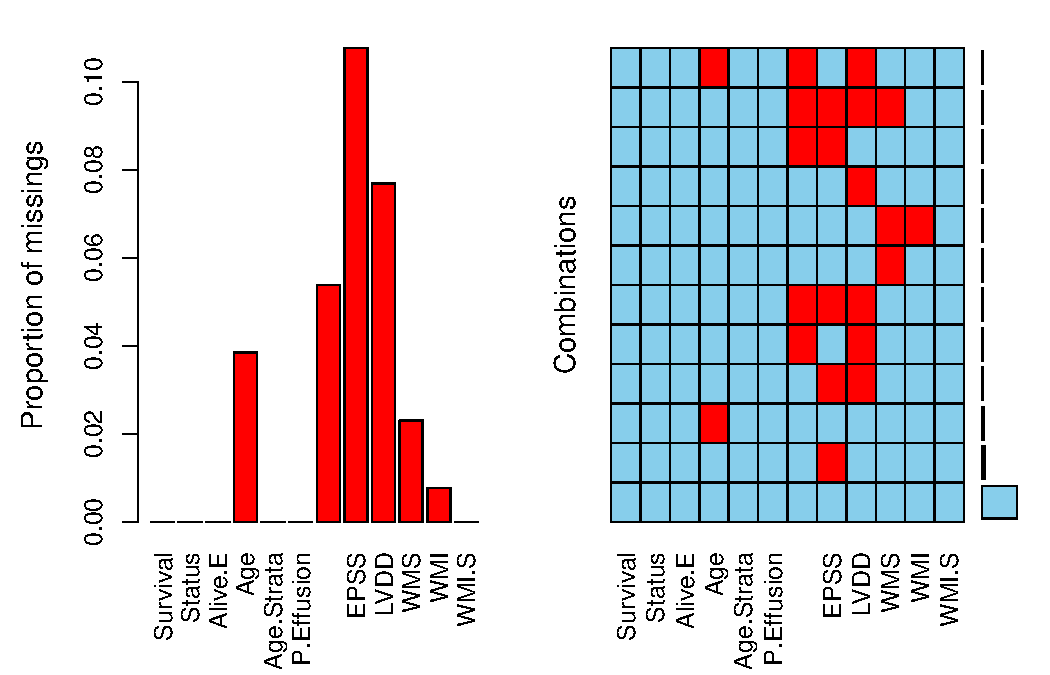
\includegraphics{markdown_files/figure-latex/missing.table-1.pdf}

We leverage the missForest package that uses algorithmic process used
here uses a modified k-nearest neighbor (KNN) approach. Using a training
data set, the routines of the algorithm predicts the missing values
trained on the observed parts of the dataset\textsuperscript{12}. The
process checks each iteration for an acceptable amount of error. If an
iteration produces an error that is smallest than that last iteration,
then the algorithm continues to function. This progress stops when an
error is larger than the previous iteration. Refer to Stekhoven, et. al
2012 for more detail.

We used the missFortune package to run up to 500 iterations. Each
iteration was allotted 1000 trees for the random forest algorithmic
approach.

Following imputation, we verify the imputation accuracy using the
normalized root mean squared error as an indicator of accuracy
(NRMSE)\textsuperscript{8}. The general performance of our imputed
dataset can be expressed by:

\[ NRMSE\ =\ \sqrt{\frac{mean\left(\left(X^{true}-X^{imp}\right)^2\right)}{var\left(X^{true}\right)}} \]

Where X is a matrix of our dataset. Being a random forest iterative
process, each imputed dataset will be different from each other. For our
particular seed and iterations, we obtained a NRMSE value of 0.1442 -
that is our inputted values have an estimate 14.42\% deviation from
estimated true accuracy.

The full imputed dataset may be found in the appendix of this paper. As
well as references to the authors who created the algorithm.

\hypertarget{censoring}{%
\subsubsection{Censoring}\label{censoring}}

Our dataset has numerous censored valued - that is, valued that cannot
be recorded due the constraint of the study design. In our data set, we
are examining the survival after a heart attack, that is, the event of
interest is death given that a patient has had already survived a heart
attack (left truncation).

We have fixed start and end dates for when the data was collection. Some
patients joined when the study began. Others joined later after the
start date. Because of this, we cannot accurately determine how long a
patient survived after our observation period is over. In addition,
there are some patients that have been lost to follow up or may have
died due to the onset of other unrelated factors. These data present
themselves as being randomly right censored.

\hypertarget{methodology}{%
\section{Methodology}\label{methodology}}

Here, we briefly review the methodology and theory behind our analysis
techniques for context.

\hypertarget{non-parametric-kaplan-meier}{%
\subsection{Non-Parametric: Kaplan
Meier}\label{non-parametric-kaplan-meier}}

We use Kaplan-Meier (KM) survival estimators to model a step curve for
the survival of our censored dataset. The KM estimator is an adjustment
of an empirical survival function to reflect the presence of
right-censored observations\textsuperscript{14}. The estimator can be
described in the following equation:

\[ \hat{S}(t) = \prod_{y_{(i)}\leq{t}}^{k} p_i = \prod_{i=1}^{k} (\frac{n_i -d_i}{n_i}) \]

Where \(n_i\) is the number alive before time \(y_i\) and \(d_i\) is the
number of events during during that interval. In our case, \(y_i\) is
the specific patient being observed, \(n_i\) is the number of patients
alive at time \(y_i\). With \(k = 131\), our KM equation is:

\[ \hat{S}(t) = \prod_{i=1}^{131} (\frac{n_i -d_i}{n_i}) \]

We use this equation to estimate the survival at each time interval. We
conduct this analysis for the whole data set and then choose to stratify
on age, pericardial effusion presence, and wall motion score. We also
include cumulative hazard estimators based on the KM fit. Additionally,
as we stratify groups by covariates, we use the Mantel-Haenszel/log-rank
test. The following equation is used to calculate the test statistic in
order to compare two strata\textsuperscript{14}:

\[ Mantel-Haenszel Statistic = \frac
{\sum_{i=1}^{k} (a_i-E_{0}(A_i))}
{\sqrt{\sum_{i=1}^{k} Var_0 (A_i)}}
\]

Where,

\[E_0(A) = \frac{m_1 n_1}{n} \;\; and \;\;\; Var_0(A) =\frac{m_1(n-m_1)}{n-1}*\frac{n_1}{n}(1-\frac{n_1}{n})\]

We then use the Mantel-Haenzel statistics to perform a standard
chi-square test to examine the differences between our strata.

\hypertarget{cumulative-hazard-estimator}{%
\subsubsection{Cumulative Hazard
Estimator}\label{cumulative-hazard-estimator}}

We calculate the hazard of our Kaplan-Survivor function by observing
standard cumulative hazard estimate (shown below):

\[ \hat{H}(t) = -log S(t) = -log \prod_{y_{(i)}\leq{t}} \frac{d_i - n_i}{n_i}  \]

Intuitively, the relationship of the observed hazard is the negative log
of the survival function at each interval. We can clearly see a
graphical relationship between our survival by examining our hazard
plots in the results section. There was the possibility of using
Nelson-Aalen's approximation for hazard, but we find that the
computation is trivial.

\hypertarget{parametric-modeling-of-survival-data}{%
\section{Parametric Modeling of Survival
Data}\label{parametric-modeling-of-survival-data}}

Another technique for characterizing the survival function is to assume
a distributional model for the data. Compared with the Kaplan-Meier
approach, this method has certain advantages; it enables construction of
a continuous survival curve and allows simplicity of estimation and
prediction. If the selected model accurately describes the data, it may
also lend insight into the underlying mechanism for the survival
behavior. This method is only applicable if a distributional model can
be identified that adequately fits the survival data.

For the post-myocardial infarction dataset, we fit three commonly
employed distributional models to the survival data and evaluating
goodness of fit of the three models. This is accomplished by comparing
the modeled survival curves to the Kaplan-Meier curve and by comparing
point estimates for each model.

The three models chosen for comparison are the Weibull, log-normal, and
log-logistic distributions.

The Weibull hazard function is given below, where \(\lambda\) and
\(\alpha\) are the scale and shape parameters. Weibull hazard is rising
if\(\alpha\) \textgreater{} 1, constant if \(\alpha\) = 1, and declining
if \(\alpha\) \textless{} 1.

\[ \ h(t) = {\lambda}^{-1}{(-log(1-p))}^{1/\alpha} \]

The log-normal distribution can be defined relative to the standard
normal distribution; a random variable Y may be said to have the
log-normal distribution if for some random variable T that has standard
normal distribution:

\[ log (Y) = \alpha + \sigma{T} \]

The hazard function of the log-normal distribution increases with time
from 0 until it reaches a maximum and then decreases, approaching 0 as
time approaches infinity.

The log-logistic distribution can be defined relative to the standard
logistic distribution; a random variable X may be said to have the
log-logistic distribution if for some random variable S that has
standard logistic distribution:

\[ log (X) = \alpha + \sigma{S} \]

the hazard function of the log-logistic distribution decreases with time
from \(\infty\) if \(\alpha\) \textless{} 1, decreases from \(\lambda\)
if \(\alpha\) = 1, and if \(\alpha\) \textgreater{} 1 resembles the
log-normal distribution.

\hypertarget{semi-parametric-modeling-of-survival-data}{%
\section{Semi-Parametric Modeling of Survival
Data}\label{semi-parametric-modeling-of-survival-data}}

Where fully parametric models offer flexibility and the efficient,
relatively simple estimation of overall survival function parameters,
semi-parametric models offer the advantage of being well-suited to the
estimation of covariate effects. Semi-parametric models decompose risk
into a baseline hazard component and a relative risk component that is
dependent on the covariates.

The semi-parametric Cox proportional hazards model is employed here to
explore the relationship between predictor variables and survival
behavior.

The Cox PH hazard function is defined as follows:

\[ h(t)=h_0(t)exp(b_1x_1+b_2x_2+...+b_nx_n) \]

where t represents the survival time, \(x_1,x_2,...,x_n\) are the set of
prognostic factors or covariates, and the coefficients
\(b_1,b_2,...,b_n\) measure the effect of the covariates on survival
time. The baseline hazard \(h_0(t)\) corresponds to the value of the
hazard if all covariates are equal to zero.

Use of the Cox PH model requires that the baseline hazard is not
dependent on the covariates, and that the covariate terms do not depend
on time - that is, that the slope coefficients are constant. Hazard
functions stratified on covariate group may be used to assess the
proportional hazard assumption. If the hazards functions for covariate
groups cross over time, the proportionality assumption is not met and
alternate analysis methods should be employed. One such method involves
sub-setting the survival data and covariates based on hazard cross-over
time. In this approach, a separate model is fit to each subset where it
has been determined that the proportionality assumption holds.
Alternately one may apply alternate modeling techniques that are
suitable for time-varying effects, or simply investigate the impact of
covariate by inspection of stratified Kaplan-Meier survival curves
\textsuperscript{14}.

\hypertarget{results}{%
\section{Results}\label{results}}

\hypertarget{non-parametric-kaplan-meier-survival-estimates}{%
\subsection{Non-Parametric: Kaplan-Meier Survival
Estimates}\label{non-parametric-kaplan-meier-survival-estimates}}

Kaplan-Meier estimates give us the following curve (full KM estimator
table can be found in the appendix).

\begin{center}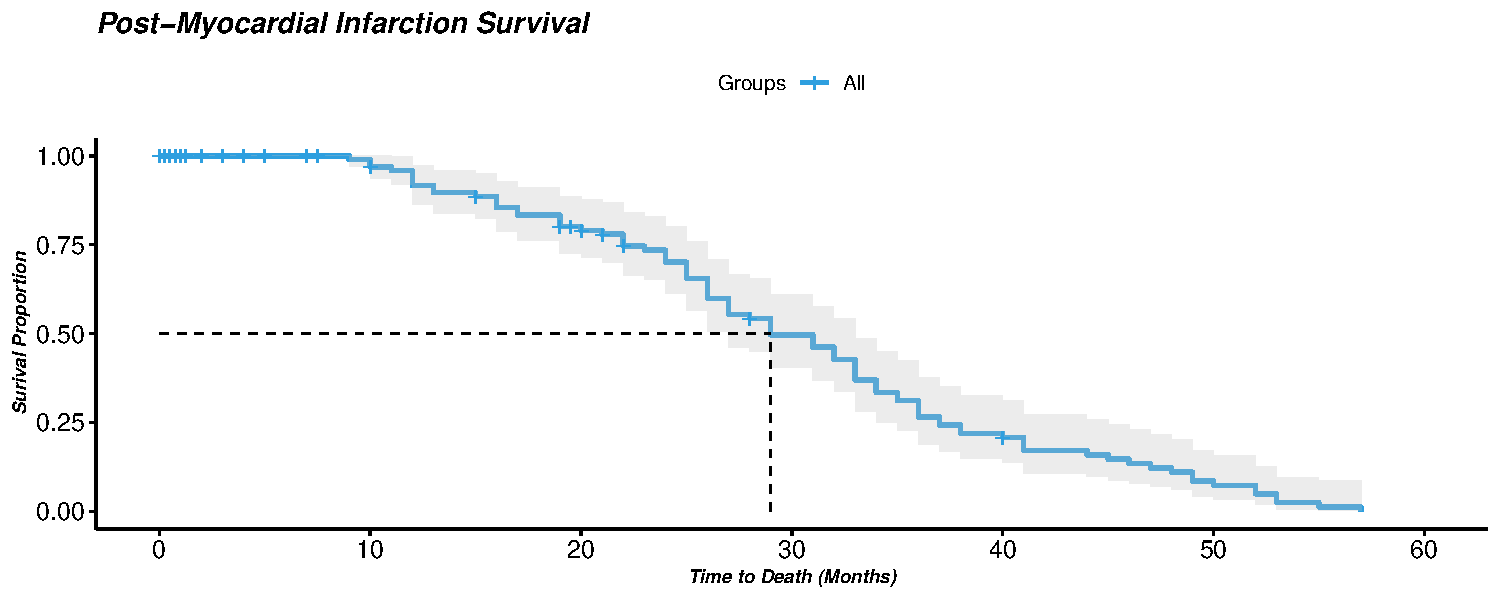
\includegraphics{markdown_files/figure-latex/km.all-1} \end{center}

\begin{table}[!h]

\caption{\label{tab:ks1}Kaplan-Meier Estimates for All Groups}
\centering
\begin{tabular}[t]{l|c|c|c|c|c|c}
\hline
  & Records & Events & Mean & Median & Median 0.95 LCL & Median 0.95 UCL\\
\hline
All Groups & 130 & 88 & 30.53 & 29 & 27 & 33\\
\hline
\end{tabular}
\end{table}

The Kaplan-Meier estimates for for all groups within our dataset is
shown above. The curve follows a general pattern of decreasing
survivability over time. With time spanning to a maximum of 57 months,
we have a mean survival time of approximately 30.5 months. The median
survival time is 29 months with 95\% confidence limits between 27 and 33
months.

When testing for significant difference between strata groups we use the
log-ran

\begin{center}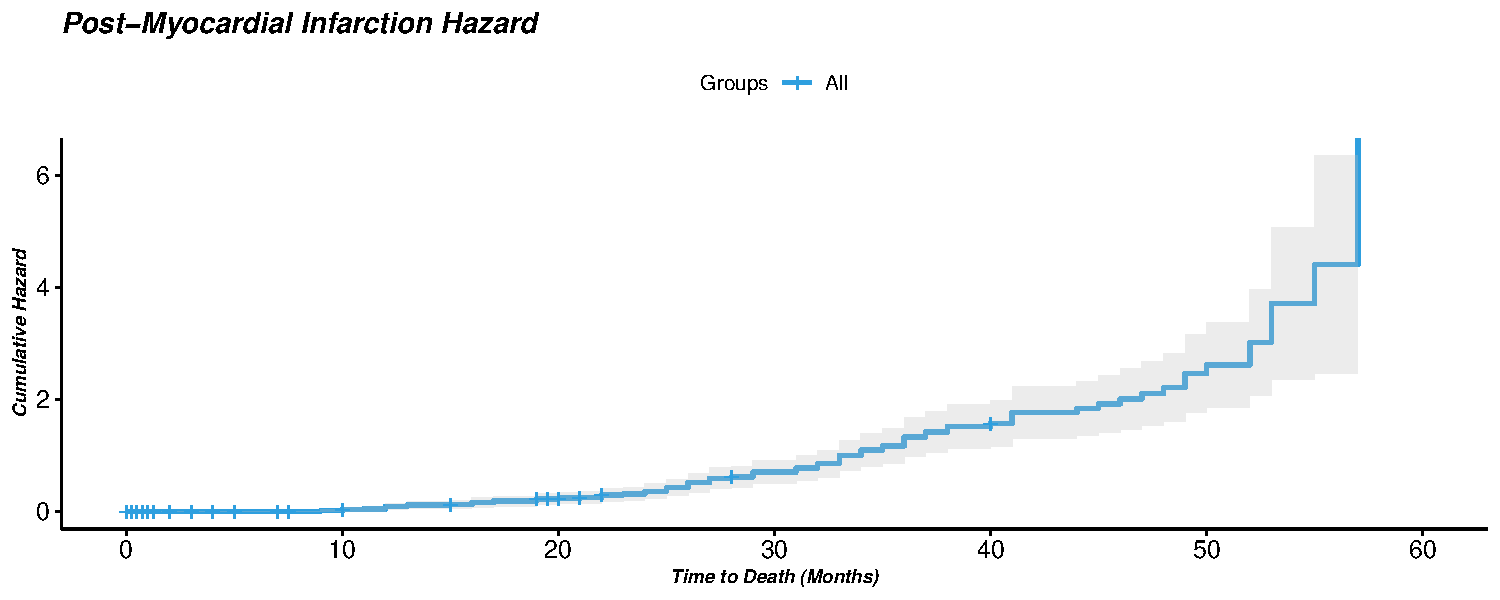
\includegraphics{markdown_files/figure-latex/kmhaz.all-1} \end{center}

To explore differences among groups, we stratify among age, pericardial
effusion presence, wall motion score, and fractional shortening. We
first begin exploring the effects of age and pericardial effusion
presence:

\hypertarget{kaplan-meier-stratified-by-age-and-pericardial-effusion-presence}{%
\subsubsection{Kaplan-Meier Stratified by Age and Pericardial Effusion
Presence}\label{kaplan-meier-stratified-by-age-and-pericardial-effusion-presence}}

The results of a Kaplan-Meier estimate for age and pericardial effusion
stratification can be seen below:

\begin{center}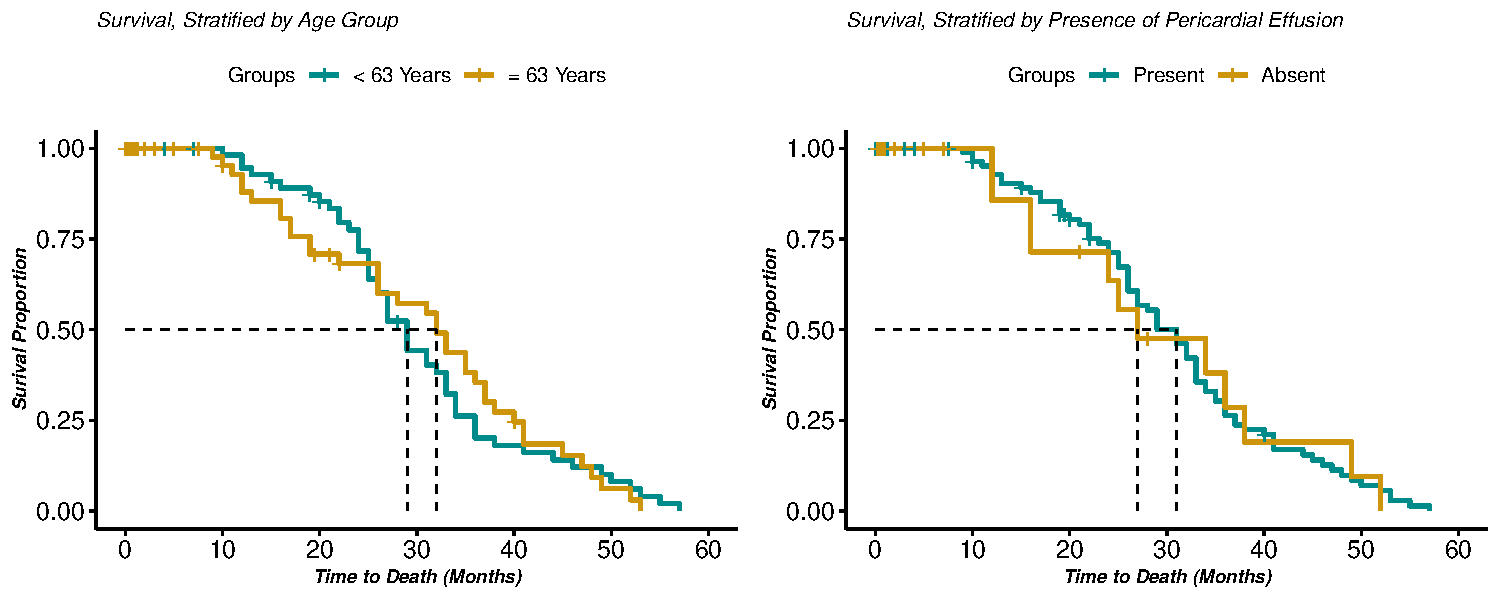
\includegraphics{markdown_files/figure-latex/km.age.effusion-1} \end{center}

\begin{table}[!h]

\caption{\label{tab:ks2}Kaplan-Meier Estimates Stratified by Age and Pericardial Effusion Presence}
\centering
\begin{tabular}[t]{l|c|c|c|c|c|c}
\hline
  & Records & Events & Mean & Median & Median 0.95 LCL & Median 0.95 UCL\\
\hline
Age < 63 & 66 & 51 & 30.47 & 29 & 26 & 33\\
\hline
Age >= 63 & 64 & 37 & 30.60 & 32 & 26 & 37\\
\hline
Absent & 106 & 76 & 30.63 & 31 & 27 & 33\\
\hline
Present & 24 & 12 & 29.94 & 27 & 24 & NA\\
\hline
\end{tabular}
\end{table}

\begin{table}

\caption{\label{tab:ks2.survdiff}Summary of Differences Between Strata}
\centering
\begin{tabular}[t]{l|r|r|r}
\hline
  & N & Observed & Expected\\
\hline
Age < 63 & 66 & 51 & 50.58084\\
\hline
Age >= 63 & 64 & 37 & 37.41916\\
\hline
Absent & 106 & 76 & 76.42260\\
\hline
Present & 24 & 12 & 11.57740\\
\hline
\end{tabular}
\end{table}

When stratified by age, we find a slight difference between the curves.
The age group younger than 63 has a mean survival time of 30.47 months
with a median survival time of 29 months. The older group - ages greater
than 63 - has a similar mean survival time of 30.6 months and a slightly
longer median survival time of 32 months. When comparing the presence of
pericardial effusion, there are 106 cases where the effusion is absent,
while 24 cases have the effusion present. The mean survival time when
pericardial effusion is absent is 30.63 months with a median survival
time of 31 months. For converse case, the mean survival time is 29.94
months while the median is lower at 27 months.

Log-rank tests between both stratification groups returns a p-value of
0.9 for both age strata and effusion strata. When testing at the 95\%
significance level, we do not have significant differences between
groups.

\begin{center}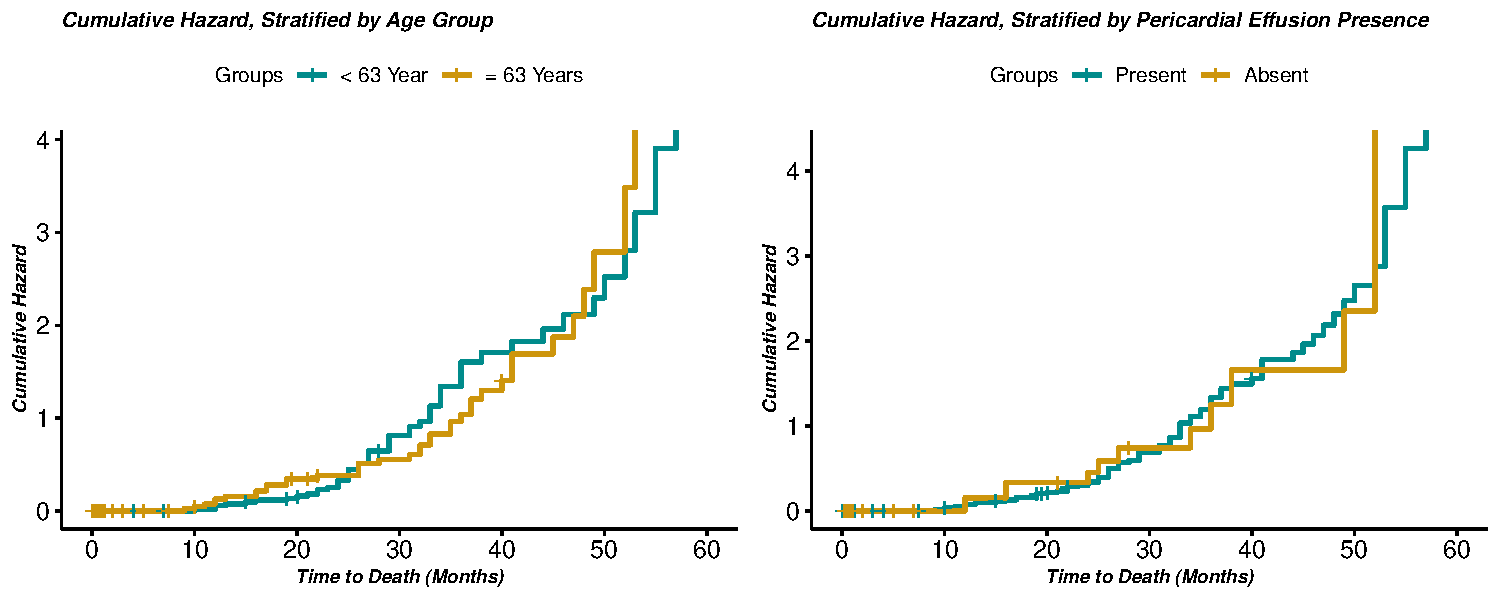
\includegraphics{markdown_files/figure-latex/km.haz1-1} \end{center}

For both groups, there does not seem to be a large departure from
cumulative hazard. When stratifying by age, we see a slight increase in
cumulative hazard of the younger group between 30 and 50 months. After
that mark, the older group experiences a relative increase in cumulative
hazard. When stratified by pericardial effusion presence, very little
difference can be observed with any difference being the result of
sample size differences.

\newpage

\hypertarget{kaplan-meier-stratified-by-wall-motion-score-and-fractional-shortening-length}{%
\subsubsection{Kaplan-Meier Stratified by Wall Motion Score and
Fractional Shortening
Length:}\label{kaplan-meier-stratified-by-wall-motion-score-and-fractional-shortening-length}}

We then explore the effects of wall motion score and fractional
shortening:

\begin{center}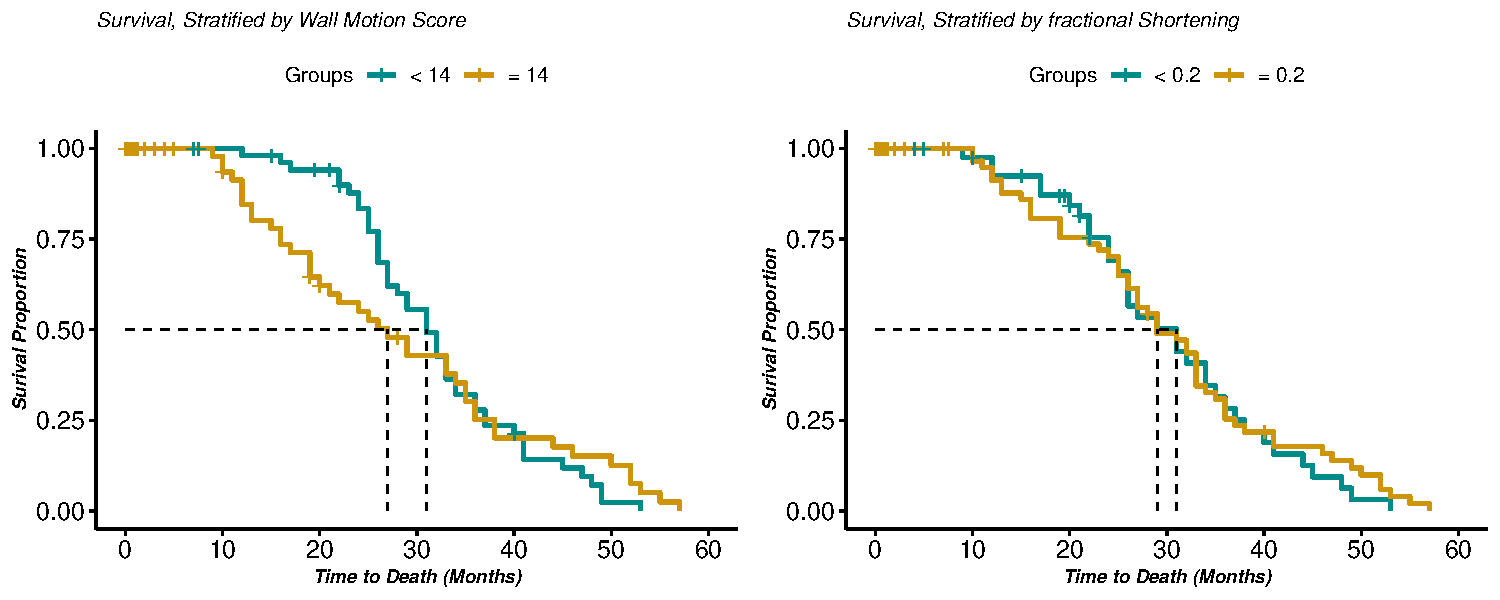
\includegraphics{markdown_files/figure-latex/km.wms.fshort-1} \end{center}

\begin{table}[!h]

\caption{\label{tab:ks4}Kaplan-Meier Estimates Stratified by Wall Motion Score and fractional Shortening}
\centering
\begin{tabular}[t]{l|c|c|c|c|c|c}
\hline
  & Records & Events & Mean & Median & Median 0.95 LCL & Median 0.95 UCL\\
\hline
Score < 14 & 62 & 46 & 32.17 & 31 & 27 & 34\\
\hline
Score >= 14 & 68 & 42 & 28.61 & 27 & 20 & 35\\
\hline
Length < 0.2 & 61 & 33 & 30.45 & 31 & 26 & 36\\
\hline
Length >= 0.2 & 69 & 55 & 30.44 & 29 & 26 & 33\\
\hline
\end{tabular}
\end{table}

\begin{table}

\caption{\label{tab:ks4.5.survdiff}Summary of Differences Between Strata}
\centering
\begin{tabular}[t]{l|r|r|r}
\hline
  & N & Observed & Expected\\
\hline
Wall Motion Score < 14 & 62 & 46 & 46.76057\\
\hline
Wall Motion Score >= 14 & 68 & 42 & 41.23943\\
\hline
Fractional Shortening < 0.2 & 61 & 33 & 30.98374\\
\hline
Fractional Shortening >= 0.2 & 69 & 55 & 57.01626\\
\hline
\end{tabular}
\end{table}

When stratified by wall motion score, we find a difference between the
curves. Wall motion scores less than 14 have a mean survival time of
32.17 months with a median survival time of 31 months. Wall motion
scores greater or equal to 14 have a lower mean survival time of 28.61
months and a median survival time of 27 months.

When stratified by fractional shortening length, both groups have a
similar mean at approximately 30.4 months. When fractional shortening is
less than 0.2, the median survival time is 31 months while having a
fractional shortening length that is greater than 0.2, we have a
slightly lower median survival time of 29 months.

Log-rank tests to test differences between wall motion score strata show
p-value of 0.9 while the same test produces a p-value of 0.6 for
fractional shortening. Both of these failures fail to reject the null
hypothesis at the 95\% significance level. As such, there is no
significant difference between either strata groupings.

\begin{center}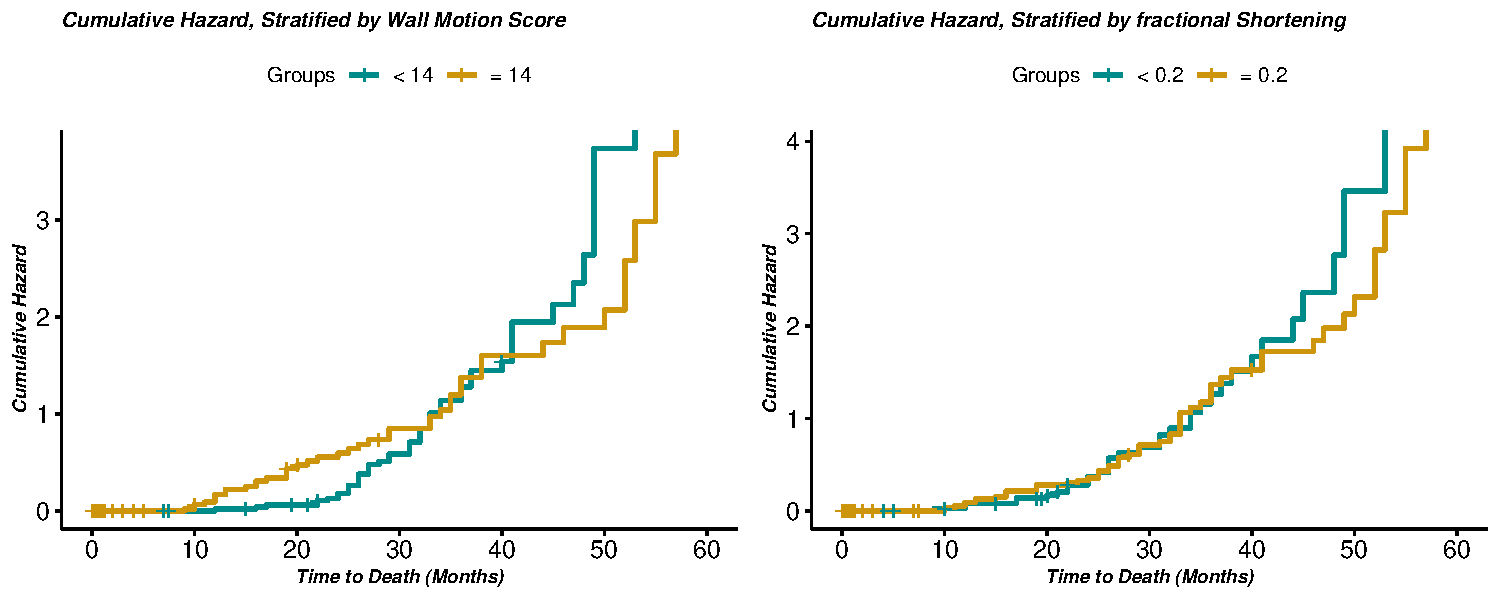
\includegraphics{markdown_files/figure-latex/km.haz2-1} \end{center}

Here, we see some minute differences between the hazard curves. When
stratified by Wall Motion Score, we see some overlap in the initial
stages of the study as well as around approximately 35 months. The
exceptions are seen with higher wall motion scores seeing increased risk
before the median and decreased relative risk after the median. The
converse is seen for the lower wall motion scores.

When stratified by fractral shortening, the cumulative hazard curves are
approximately similar with higher fractional shortening lengths have
less risk after the median.

\hypertarget{parametric-analysis-and-estimation}{%
\subsection{Parametric Analysis and
Estimation}\label{parametric-analysis-and-estimation}}

The estimated distributional model curves are overlaid on the K-M curve
for the post-myocardial infarction data in the figures below.

\begin{center}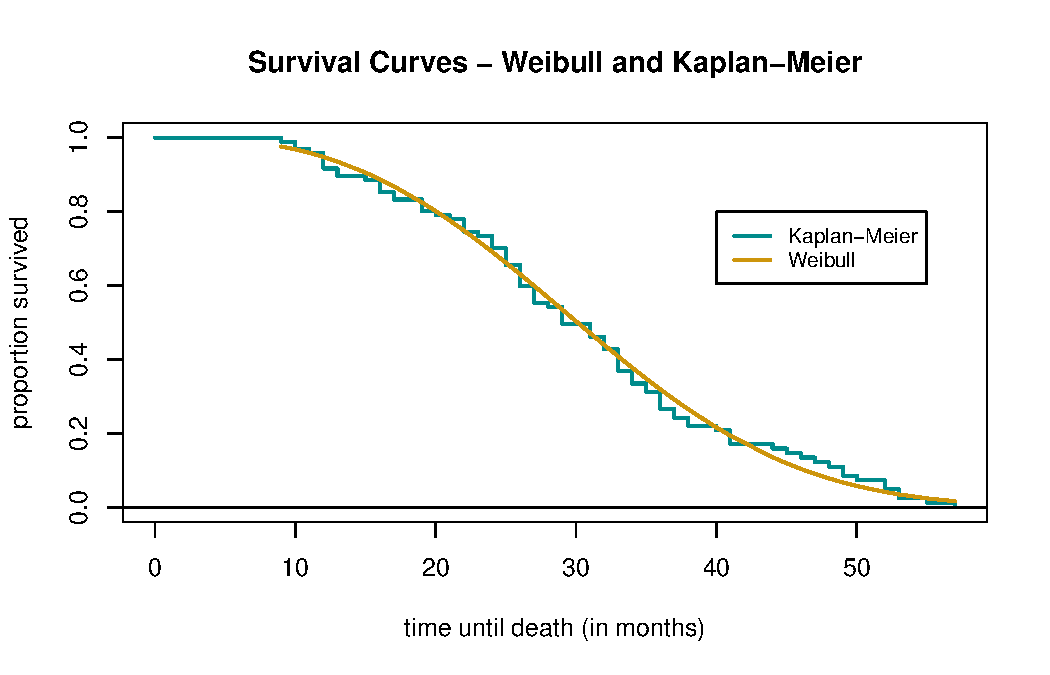
\includegraphics[width=0.75\linewidth]{markdown_files/figure-latex/unnamed-chunk-1-1} \end{center}

\begin{center}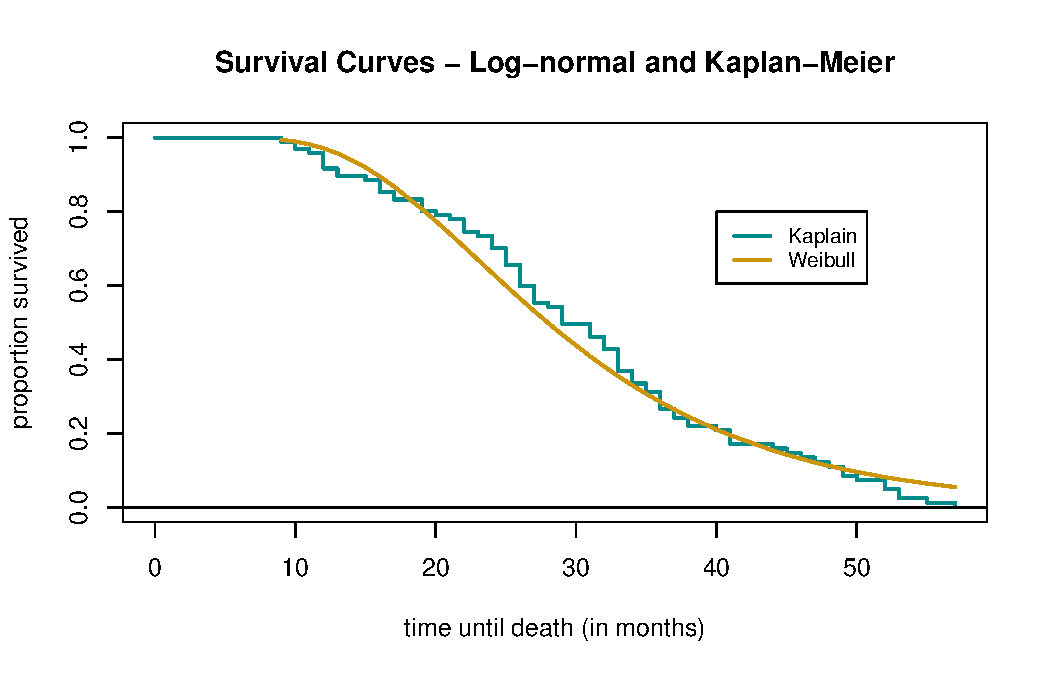
\includegraphics[width=0.75\linewidth]{markdown_files/figure-latex/unnamed-chunk-1-2} \end{center}

\begin{center}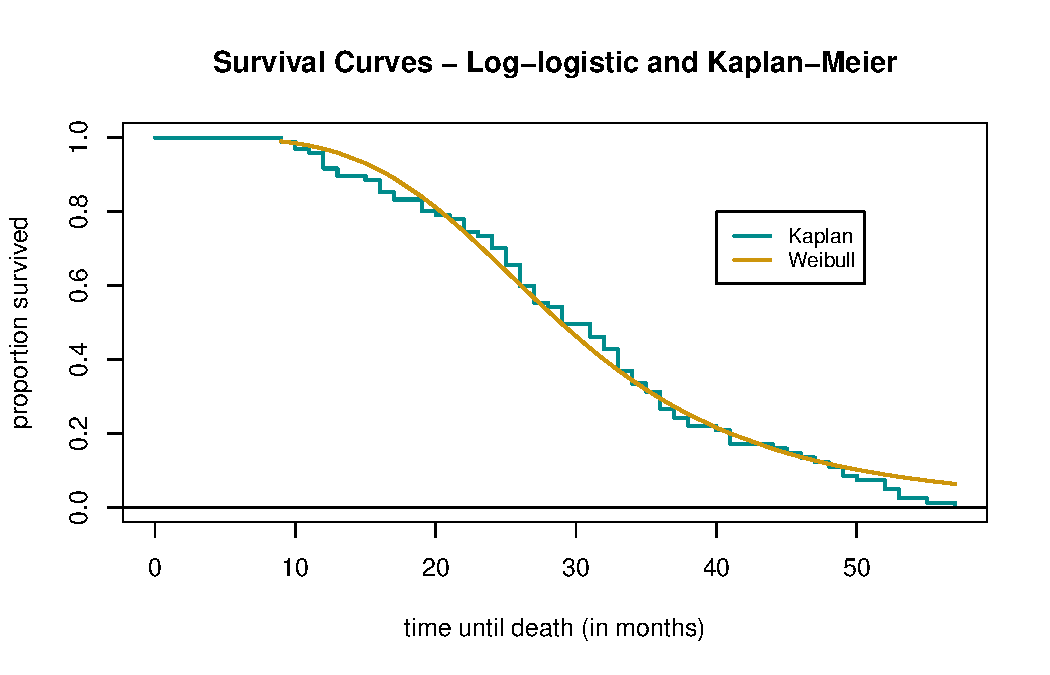
\includegraphics[width=0.75\linewidth]{markdown_files/figure-latex/unnamed-chunk-1-3} \end{center}

\newpage

The table below summarizes the parameter point estimates and
corresponding 95\% confidence intervals.

\begin{table}[H]

\caption{\label{tab:unnamed-chunk-2}Parametric Model Estimates}
\centering
\begin{tabular}[t]{c|c|c|c|c}
\hline
Quantile & Point Estimate & 95\% LCL & 95\% UCL & Interval Length\\
\hline
\multicolumn{5}{l}{\textbf{Weibull Model Fit}}\\
\hline
\hspace{1em}0.25 & 22.42 & 19.96 & 25.19 & 5.23\\
\hline
\hspace{1em}0.50 & 30.32 & 27.86 & 33.01 & 5.15\\
\hline
\hspace{1em}0.75 & 38.47 & 35.71 & 41.44 & 5.72\\
\hline
\multicolumn{5}{l}{\textbf{Log-normal Model Fit}}\\
\hline
\hspace{1em}0.25 & 20.73 & 18.77 & 22.89 & 4.11\\
\hline
\hspace{1em}0.50 & 27.97 & 25.54 & 30.63 & 5.09\\
\hline
\hspace{1em}0.75 & 37.74 & 34.06 & 41.83 & 7.77\\
\hline
\multicolumn{5}{l}{\textbf{Log-logistic Model Fit}}\\
\hline
\hspace{1em}0.25 & 21.90 & 19.77 & 24.27 & 4.50\\
\hline
\hspace{1em}0.50 & 28.88 & 26.41 & 31.59 & 5.18\\
\hline
\hspace{1em}0.75 & 38.09 & 34.45 & 42.12 & 7.67\\
\hline
\end{tabular}
\end{table}

Q-Q plots were also prepared for each distribution, and are provided in
the Appendix. Based on inspection of the Q-Q plots and the K-M overlay
plots, we found that the Weibull model appears to provide the best fit.
In addition, it was noted that the confidence intervals for point
estimation were overall more narrow for the Weibull model compared to
log-normal and log-logistic. It was also observed that the point
estimate for median is close to that identified by the Kaplan-Meier
approach (29 months in K-M estimation, 30 months when estimating with
Weibull fit). We propose the Weibull model as descriptive of the
post-myocardial infarction survival data.

\hypertarget{regression-analysis---cox-proportional-hazard-modeling}{%
\subsection{Regression Analysis - Cox Proportional Hazard
Modeling}\label{regression-analysis---cox-proportional-hazard-modeling}}

Regression analysis was conducted to identify the relationship between
potential predictor variables and survival. As a first step, the
covariate pool was screened for potential multicollinearity (see
Appendix for plots of the covariates). Potential dependency was observed
between Fractional Shortening, E-Point Septal Separation, and Left
Ventrical Diastolic Dysfunction. Mechanistically, this is intuitive,
since all three variables measure ventrical diastolic behavior. Models
were fit with each of these collinear variables, and based on this
assessment of Fractional Shortening was selected for inclusion in the
final covariate pool of potential prognostic factors for regression.
These covariates are:

\begin{description}
  \item[$\bullet$] Age
  \item[$\bullet$] Pericardial Effusion
  \item[$\bullet$] Wall Motion Score
  \item[$\bullet$] Fractional Shortening
\end{description}

A model employing all of the covariates listed above was created. In
order to test validity of the proportional hazard assumption, survival
curves stratified by group were assessed for each of the four selected
covariates. It was found that the proportional hazard assumption does
not hold, as hazards for each group cross over with time for each
covariate.

This limitation was addressed through the identification of survival
time subsets in which covariates met the proportional hazards
assumption, and could thus be employed as predictor variables. These
subsets were identified by inspecting hazard function data stratified on
all covariates and identifying regions of crossover. (See Appendix for
plots of stratified hazard functions with the approximate crossover
regions marked).

The selected time subsets were obtained as follows:

\begin{description}
 \item[$Subset \:1: t \leq {26} \:{months}$]
 \item[$Subset \:2:26 \:{months}< t < 46 \:{months}$]
 \item[$Subset \:3: 46 \: months \leq t$]
\end{description}

Within each time subset, the proportional hazard assumption was tested
for each of the four covariates and found to hold. A Cox PH model was
fitted to each subset of the survival data, reduced as far as possible
using a Step AIC procedure up to second order interactions with
Likelihood Ratio Test selection of the final model, and evaluated for
adequacy using standard diagnostic techniques.

The three models are summarized below:

\begin{table}[H]

\caption{\label{tab:unnamed-chunk-3}Summary of CoxPH Regression Models}
\centering
\begin{tabular}[t]{c|c|c|c|c|c|c|c|c|c}
\hline
\multicolumn{1}{c|}{ } & \multicolumn{3}{c|}{Model 1} & \multicolumn{3}{c|}{Model 2} & \multicolumn{3}{c}{Model 3} \\
\cline{2-4} \cline{5-7} \cline{8-10}
\multicolumn{1}{c|}{\bgroup\fontsize{8}{10}\selectfont  \egroup{}} & \multicolumn{3}{c|}{\bgroup\fontsize{8}{10}\selectfont LRT = 10.34 on 3 df; p = 0.02\egroup{}} & \multicolumn{3}{c|}{\bgroup\fontsize{8}{10}\selectfont LRT = 13.9 on 1 df; p = 0.05\egroup{}} & \multicolumn{3}{c}{\bgroup\fontsize{8}{10}\selectfont LRT = 10.34 on 1 df; p = 0.1\egroup{}} \\
\cline{2-4} \cline{5-7} \cline{8-10}
\multicolumn{1}{c|}{\bgroup\fontsize{8}{10}\selectfont  \egroup{}} & \multicolumn{3}{c|}{\bgroup\fontsize{8}{10}\selectfont n = 77; \#events = 37\egroup{}} & \multicolumn{3}{c|}{\bgroup\fontsize{8}{10}\selectfont n = 42; \#events = 40\egroup{}} & \multicolumn{3}{c}{\bgroup\fontsize{8}{10}\selectfont n = 11; \#events = 11\egroup{}} \\
\cline{2-4} \cline{5-7} \cline{8-10}
Covariate & HR & 95\% CI & p-val & HR & 95\% CI & p-val & HR & 95\% CI & p-val\\
\hline
FS & 0.85 & (0.69, 1.05) & 0.13 &  &  &  & 0.9 & (0.79, 1.02) & 0.11\\
\hline
WMS & 0.00 & (0.00, 0.01) & 9 &  &  &  &  &  & \\
\hline
WMS*FS & 4.31 & (1.51, 12.4) & 006 &  &  &  &  &  & \\
\hline
Age &  &  &  & 0.96 & (0.92, 1.00) & 0.051 &  &  & \\
\hline
 &  &  &  &  &  &  &  &  & \\
\hline
\end{tabular}
\end{table}

For Model 1, the significant predictors of survival time are identified
as Fractional Shortening and its interaction with Wall Motion Score.
Although Wall Motion Score does not have a significant effect on
survival as a main effect, it is retained due to is presence in the
interaction term.

For Model 2, the significant predictor of survival time is identified as
patient age. Age is found to have a very weak effect on survival; none
of the echocardiographic covariates had an impact on survival in this
time region. Both these findings are supported by inspection of the
stratified hazard function plots.

For subset 3, the sample size of events in the survival data subset was
small (n=11) and a significant model was not obtained. The model is
presented for context but is poorly descriptive of the relationship
between prognostic factors and survival.

Model residual diagnostics were assessed for all three models. Models 1
and 2 showed overall good fit to the data and demonstrated proportional
hazard assumption compliance. As expected given the discussion above,
Model 3 did not result in a good overall fit, although proportional
hazard assumption was met. Model diagnostic residual plots and further
discussion may be found in the Appendix.

\hypertarget{discussion}{%
\section{Discussion}\label{discussion}}

\hypertarget{explanation-of-results}{%
\subsection{Explanation of results}\label{explanation-of-results}}

In our non-parametric analysis, median survival times for nearly all of
the stratification elements show relatively similar results with the
exception of high wall motion scores. When stratified by age group, we
see relatively similar survival proportions with some distinction before
and after the median. Before the median, the older group has a slightly
lower survival proportion. However, after the median, the older group
has a slightly higher survival proportion before 45 months. This slight
discrepancy could be due to the externalities attached to young heart
attack patients. If patients are experiencing heart attacks at a younger
age, there could be higher chances that those patients already have
other health concerns. Patients experiencing and surviving a heart
attack at older ages could be in physically superior condition than
their younger counterparts. All other stratification groups show
relatively similar median survival proportions. An interesting
observation can be seen when we arbitrarily divide the age strata into
three groups. We see a much greater risk associated with patients
younger than 55 while all other age groups perform similarly.

In the parametric analysis, it was found that the survivor data is
well-described by the Weibull distribution. This finding enables the
construction of a continuous survivor function and provides the
opportunity for flexible point estimation as well as estimation of
survival probability over a given input time. Semi-parametric modeling
was also performed. Three Cox Proportional Hazards models were developed
that described the relationship between prognostic factors and survival;
one for short survival times; one for intermediate survival times; and
another for long survival times. Given a small sample size for long
survival times, only the first two models were significant. A key
finding from this analysis is that when survival time is shorter,
abnormalities in the echocardiographic profile of the patient's heart
are what predict survival, rather than age. Conversely, when the
survival times are longer, it is the age of the patient that predicts
survival (albeit weakly), rather than any of the echocardiographic
properties do not. This is consistent with the behavior of the
stratified hazard curves for these variables over time. This result
seems to imply that in the acute recovery period following a myocardial
infarction, patient prognosis is closely tied to heart health; but as
time progresses, patient age becomes the key driver of prognosis. This
finding is intuitive, since as treatment and recovery progress over
time, risk related to the myocardial event would decrease and other
pre-existing risks would play a larger role in survival.

\hypertarget{summary-of-limitations}{%
\subsection{Summary of Limitations}\label{summary-of-limitations}}

Very clearly, our data is smaller than we hoped for, both in the number
of observations and in the availability of meaningful prognostic
factors. Development of a single large regression fit that reliably
predicts covariates would require a much larger dataset. In particular,
the lack of gender as an available covariate is a potential limitation
of our data, as the effect of gender on heart-related survival is well
established in the literature. Longer collection period over a greater
number of patients would yield stronger regression model development.
As-is, there is not enough data to produce a significant model across
the entire survival time window.

A particular limitation related to subgroup dimension was identified
through the stratification analysis. Examination of stratified data
showed relative unequal distributions among groups. For example, when
examining pericardial effusion, we compare 106 records of with effusion
absent to 24 records of effusion present. Given that the collection
methods are unclear and the groups sizes are so much different form each
other, we cannot fully be confident in our results. Such comparisons are
unequal comparisons.

Finally, the given dataset did not have clear statements as to what data
collection methods were used. Given our smaller sample size and these
unknown methods, we cannot be entirely confident that our results
reflect the survival behavior of the population as a whole. Future
studies would benefit greatly

\hypertarget{conclusion}{%
\subsection{Conclusion}\label{conclusion}}

This study identified a variety of properties of the post-myocardial
infarction survival data. The overall survival function was
characterized by both non-parametric Kaplan-Meier and Weibull models,
and point estimates determined. Analysis of the effect of
echocardiographic data and of age on survival was performed both by
inspection of stratified survival curves and by regression analysis.
Findings included that age group has an impact on survival, but that
this effect potentially varies over time, and that certain heart-related
prognostic factors (in particular wall motion score and its interaction
with fractional shortening) also have an impact on survival that varies
over time. We conclude that future studies should expand on collection
of variables that could potentially influence survivability, as well as
the cohort size and length of follow-up period. Interesting effects to
include may include poverty, diet, ethnicity, race, sex, and even work
place stress/effects. Finally, further investigation with a larger
dataset on the relationship between acute survival time and
echocardiographic data profile and between the relationship of age group
on survival data may yield useful insights into specific risk profiles
for post-myocardial infarction patients.

\newpage

\hypertarget{appendix}{%
\section{Appendix}\label{appendix}}

\hypertarget{references}{%
\subsection{References}\label{references}}

\begin{enumerate}
\def\labelenumi{\arabic{enumi}.}
\item
  Andrikopoulos, G. K., Tzeis, S. E., Pipilis, A. G., Richter, D. J.,
  Kappos, K. G., Stefanadis, C. I., \ldots{} Chimonas, E. T. (2006).
  Younger age potentiates post myocardial infarction survival
  disadvantage of women. International Journal of Cardiology, 108(3),
  320--325. doi: 10.1016/j.ijcard.2005.05.016
\item
  Fryar CD, Chen T-C, Li X. Prevalence of uncontrolled risk factors for
  cardiovascular disease: United States, 1999--2010 pdf
  icon{[}PDF-494K{]}. NCHS data brief, no. 103. Hyattsville, MD:
  National Center for Health Statistics; 2012. Accessed May 9, 2019.
\item
  Ford, E. S., \& Capewell, S. (2007). Coronary Heart Disease Mortality
  Among Young Adults in the U.S. From 1980 Through 2002. Journal of the
  American College of Cardiology, 50(22), 2128--2132. doi:
  10.1016/j.jacc.2007.05.056
\item
  Dalen JE, Alpert JS, Goldberg RJ, Weinstein RS. The epidemic of the
  20(th) century: coronary heart disease. Am J Med. 2014;127(9):807‐812.
  \url{doi:10.1016/j.amjmed.2014.04.015}
\item
  Goldman, L. (1984). The Decline in Ischemic Heart Disease Mortality
  Rates. Annals of Internal Medicine, 101(6), 825. doi:
  10.7326/0003-4819-101-6-825
\item
  Gu K, Cowie CC, Harris MI. Diabetes and Decline in Heart Disease
  Mortality in US Adults. JAMA. 1999;281(14):1291--1297.
  \url{doi:10.1001/jama.281.14.1291}
\item
  Heron, M. Deaths: Leading causes for 2017 pdf icon{[}PDF -- 3 M{]}.
  National Vital Statistics Reports;68(6). Accessed November 19, 2019.
\item
  Kan, G., Visser, C., Kooler, J., \& Dunning, A. (1986). Short and long
  term predictive value of wall motion score in acute myocardial
  infarction. British Heart Journal, 56, 422-427.
\item
  Oba S, Sato MA, Takemasa I, Monden M, Matsubara K, Ishii S. A Bayesian
  missing value estimation method for gene expression profile data.
  Bioinformatics. 2003;19(16):2088‐2096.
  \url{doi:10.1093/bioinformatics/btg287}
\item
  Rimm, E. B., Stampfer, M. J., Giovannucci, E., Ascherio, A.,
  Spiegelman, D., Colditz, G. A., \& Willett, W. C. (1995). Body Size
  and Fat Distribution as Predictors of Coronary Heart Disease among
  Middle-aged and Older US Men. American Journal of Epidemiology,
  141(12), 1117--1127. doi: 10.1093/oxfordjournals.aje.a117385
\item
  Salzberg, S. (1988). Exemplar-based learning: Theory and
  implementation (Technical Report TR-10-88). Harvard University, Center
  for Research in Computing Technology, Aiken Computation Laboratory (33
  Oxford Street; Cambridge, MA 02138).
\item
  Sia, Y. T., Parker, T. G., Liu, P., Tsoporis, J. N., Adam, A., \&
  Rouleau, J. L. (2002). Improved post-myocardial infarction survival
  with probucol in rats: Effects on left ventricular function,
  morphology, cardiac oxidative stress and cytokine expression. Journal
  of the American College of Cardiology, 39(1), 148--156. doi:
  10.1016/s0735-1097(01)01709-0
\item
  Stekhoven, D. J., \& Buhlmann, P. (2011). MissForest--non-parametric
  missing value imputation for mixed-type data. Bioinformatics, 28(1),
  112--118. doi: 10.1093/bioinformatics/btr597
\item
  Tableman, M., \& Kim, J. S. (2004). Survival analysis using S:
  analysis of time-to-event data. Boca Raton, Florida: Chapman \& Hall.
\item
  Wilmot, K. A., O'Flaherty, M., Capewell, S., Ford, E. S., \&
  Vaccarino, V. (2015). Coronary Heart Disease Mortality Declines in the
  United States From 1979 Through 2011CLINICAL PERSPECTIVE. Circulation,
  132(11), 997--1002. doi: 10.1161/circulationaha.115.015293
\end{enumerate}

\newpage

\hypertarget{dataset-variable-summary}{%
\subsection{Dataset Variable Summary}\label{dataset-variable-summary}}

\begin{longtabu} to \linewidth {>{\raggedright}X>{\raggedright}X>{\raggedright}X}
\caption{\label{tab:Dataset.summary}Summary of Dataset Covariates}\\
\toprule
Variable & Label & Definition\\
\midrule
\endfirsthead
\caption[]{Summary of Dataset Covariates \textit{(continued)}}\\
\toprule
Variable & Label & Definition\\
\midrule
\endhead
\
\endfoot
\bottomrule
\endlastfoot
Survival & Survival & The number of months the patints survived, post-myocardial infarction.\\
\addlinespace
Status & Status & Censorship status. 0 denotes that a patient is a censored while 1 denotes that a patient is uncensored.\\
\addlinespace
Alive at the end of Survival Period & Alive.E & Binary variable. 0 denotes that patient is alive at the end of the survival period while 1 indicates that a patient is still alive.\\
\addlinespace
Patient Age & Age & The age in years when a myocardial infarction occurs.\\
\addlinespace
Age Group & Age.S & 0 denotes younger than 55 years . 1 denotes 55 - 70 years. 2 denotes older than 70\\
\addlinespace
Pericardial Effusion & P.Effusion & Binary variable. Pericardial effusion is excess fluid surrounding the heart. Though excess is not harmful, it is sometimes indicates a porly functioning heart. 0 denotes that pericardial effusion is absent while 1 denotes that fluid is present.\\
\addlinespace
Fractional Shortening & F.Shortening & Fractional shortening is a measure of contractility around the heart. Generally, lower numbers are considered to be abnormal.\\
\addlinespace
E-Point Septal Separation & EPSS & E-point septal separation is an addition measure of heart contractivity. Larger numbers are considered to be abnormal.\\
\addlinespace
Left Ventricular End-Diastolic Dimension & LVDD & Left ventricular end-diastolic dimension is the measure of the heart at the end of disatole. The larger this value is indicates a larger heart. Larger hearts are generally in poor health.\\
\addlinespace
Wall Motion Score & WMS & Wall motion score is a measure of how the segments of the left ventricle are moving during systol.\\
\addlinespace
Wall Motion Index & WMI & Wall motion index is the wall motion score divided by the number of segments that are moving. Normally, 12-13 segments can be seen in an echocardiogram.\\
\addlinespace
Wall Motion Strata & WMS.S & 0 denotes score less than 11, 1 denotes score 12-14, 2 denotes score greater than 14\\*
\end{longtabu}

\hypertarget{original-dataset}{%
\subsection{Original Dataset}\label{original-dataset}}

\begin{longtabu} to \linewidth {>{\raggedleft}X>{\raggedleft}X>{\raggedleft}X>{\raggedleft}X>{\raggedleft}X>{\raggedleft}X>{\raggedleft}X>{\raggedleft}X>{\raggedleft}X>{\raggedleft}X>{\raggedleft}X>{\raggedleft}X}
\caption{\label{tab:Dataset.actual}Original Dataset}\\
\toprule
Survival & Status & Alive.E & Age & Age.Strata & P.Effusion & F.Shortening & EPSS & LVDD & WMS & WMI & WMI.S\\
\midrule
\endfirsthead
\caption[]{Original Dataset \textit{(continued)}}\\
\toprule
Survival & Status & Alive.E & Age & Age.Strata & P.Effusion & F.Shortening & EPSS & LVDD & WMS & WMI & WMI.S\\
\midrule
\endhead
\
\endfoot
\bottomrule
\endlastfoot
11.00 & 1 & 0 & 71.00 & 2 & 0 & 0.260 & 9.000 & 4.600 & 14.00 & 1.000 & 0\\
19.00 & 1 & 0 & 72.00 & 2 & 0 & 0.380 & 6.000 & 4.100 & 14.00 & 1.700 & 1\\
16.00 & 1 & 0 & 55.00 & 1 & 0 & 0.260 & 4.000 & 3.420 & 14.00 & 1.000 & 0\\
57.00 & 1 & 0 & 60.00 & 1 & 0 & 0.253 & 12.062 & 4.603 & 16.00 & 1.450 & 1\\
19.00 & 0 & 1 & 57.00 & 1 & 0 & 0.160 & 22.000 & 5.750 & 18.00 & 2.250 & 1\\
\addlinespace
26.00 & 1 & 0 & 68.00 & 2 & 0 & 0.260 & 5.000 & 4.310 & 12.00 & 1.000 & 0\\
13.00 & 1 & 0 & 62.00 & 1 & 0 & 0.230 & 31.000 & 5.430 & 22.50 & 1.875 & 1\\
50.00 & 1 & 0 & 60.00 & 1 & 0 & 0.330 & 8.000 & 5.250 & 14.00 & 1.000 & 0\\
19.00 & 1 & 0 & 46.00 & 0 & 0 & 0.340 & 0.000 & 5.090 & 16.00 & 1.140 & 0\\
25.00 & 1 & 0 & 54.00 & 1 & 0 & 0.140 & 13.000 & 4.490 & 15.50 & 1.190 & 0\\
\addlinespace
10.00 & 0 & 1 & 77.00 & 2 & 0 & 0.130 & 16.000 & 4.230 & 18.00 & 1.800 & 1\\
52.00 & 1 & 0 & 62.00 & 1 & 1 & 0.450 & 9.000 & 3.600 & 16.00 & 1.140 & 0\\
52.00 & 1 & 0 & 73.00 & 2 & 0 & 0.330 & 6.000 & 4.000 & 14.00 & 1.000 & 0\\
44.00 & 1 & 0 & 60.00 & 1 & 0 & 0.150 & 10.000 & 3.730 & 14.00 & 1.000 & 0\\
0.50 & 0 & 1 & 62.00 & 1 & 0 & 0.120 & 23.000 & 5.800 & 11.67 & 2.330 & 1\\
\addlinespace
24.00 & 1 & 0 & 55.00 & 1 & 1 & 0.250 & 12.063 & 4.290 & 14.00 & 1.000 & 0\\
0.50 & 0 & 1 & 69.00 & 2 & 1 & 0.260 & 11.000 & 4.650 & 18.00 & 1.640 & 1\\
0.50 & 0 & 1 & 62.53 & 1 & 1 & 0.070 & 20.000 & 5.200 & 24.00 & 2.000 & 1\\
22.00 & 0 & 1 & 66.00 & 2 & 0 & 0.090 & 17.000 & 5.819 & 8.00 & 1.333 & 1\\
1.00 & 0 & 1 & 66.00 & 2 & 1 & 0.220 & 15.000 & 5.400 & 27.00 & 2.250 & 1\\
\addlinespace
0.75 & 0 & 1 & 69.00 & 2 & 0 & 0.150 & 12.000 & 5.390 & 19.50 & 1.625 & 1\\
0.75 & 0 & 1 & 85.00 & 2 & 1 & 0.180 & 19.000 & 5.460 & 13.83 & 1.380 & 1\\
0.50 & 0 & 1 & 73.00 & 2 & 0 & 0.230 & 12.733 & 6.060 & 7.50 & 1.500 & 1\\
5.00 & 0 & 1 & 71.00 & 2 & 0 & 0.170 & 0.000 & 4.650 & 8.00 & 1.000 & 0\\
48.00 & 1 & 0 & 64.00 & 1 & 0 & 0.190 & 5.900 & 3.480 & 10.00 & 1.110 & 0\\
\addlinespace
29.00 & 1 & 0 & 54.00 & 1 & 0 & 0.300 & 7.000 & 3.850 & 10.00 & 1.667 & 1\\
29.00 & 1 & 0 & 35.00 & 0 & 0 & 0.300 & 5.000 & 4.170 & 14.00 & 1.000 & 0\\
29.00 & 1 & 0 & 55.00 & 1 & 0 &  & 7.000 &  & 2.00 & 1.000 & 0\\
0.25 & 0 & 1 & 75.00 & 2 & 0 &  &  &  &  & 1.000 & 0\\
36.00 & 1 & 0 & 55.00 & 1 & 1 & 0.210 & 4.200 & 4.160 & 14.00 & 1.560 & 1\\
\addlinespace
1.00 & 0 & 1 & 65.00 & 2 & 0 & 0.150 &  & 5.050 & 10.00 & 1.000 & 0\\
1.00 & 0 & 1 & 52.00 & 1 & 1 & 0.170 & 17.200 & 5.320 & 14.00 & 1.170 & 0\\
3.00 & 0 & 1 &  & 2 & 0 &  & 12.000 &  & 6.00 & 3.000 & 1\\
27.00 & 1 & 0 & 47.00 & 0 & 0 & 0.400 & 5.120 & 3.100 & 12.00 & 1.000 & 0\\
35.00 & 1 & 0 & 63.00 & 1 & 0 &  & 10.000 &  & 14.00 & 1.170 & 0\\
\addlinespace
26.00 & 1 & 0 & 61.00 & 1 & 0 & 0.610 & 13.100 & 4.070 & 13.00 & 1.625 & 1\\
16.00 & 1 & 0 & 63.00 & 1 & 1 &  &  & 5.310 & 5.00 & 1.000 & 0\\
1.00 & 0 & 1 & 65.00 & 2 & 0 & 0.060 & 23.600 &  & 21.50 & 2.150 & 1\\
19.00 & 1 & 0 & 68.00 & 2 & 0 & 0.510 &  & 3.880 & 15.00 & 1.670 & 1\\
31.00 & 1 & 0 & 80.00 & 2 & 0 & 0.410 & 5.400 & 4.360 &  & 1.000 & 0\\
\addlinespace
32.00 & 1 & 0 & 54.00 & 1 & 0 & 0.350 & 9.300 & 3.630 & 11.00 & 1.222 & 0\\
16.00 & 1 & 0 & 70.00 & 2 & 1 & 0.270 & 4.700 & 4.490 & 22.00 & 2.000 & 1\\
40.00 & 1 & 0 & 79.00 & 2 & 0 & 0.150 & 17.500 & 4.270 & 13.00 & 1.300 & 1\\
46.00 & 1 & 0 & 56.00 & 1 & 0 & 0.330 &  & 3.590 & 14.00 & 1.000 & 0\\
2.00 & 0 & 1 & 67.00 & 2 & 1 & 0.440 & 9.000 & 3.960 & 17.50 & 1.450 & 1\\
\addlinespace
37.00 & 1 & 0 & 64.00 & 1 & 0 & 0.090 &  &  & 12.00 & 2.000 & 1\\
19.50 & 0 & 1 & 81.00 & 2 & 0 & 0.120 &  &  & 9.00 & 1.250 & 0\\
20.00 & 0 & 1 & 59.00 & 1 & 0 & 0.030 & 21.300 & 6.290 & 17.00 & 1.310 & 1\\
0.25 & 0 & 1 & 63.00 & 1 & 1 &  &  &  & 23.00 & 2.300 & 1\\
2.00 & 0 & 1 & 56.00 & 1 & 1 & 0.040 & 14.000 & 5.000 &  &  & 1\\
\addlinespace
7.00 & 0 & 1 & 61.00 & 1 & 1 & 0.270 &  &  & 9.00 & 1.500 & 1\\
10.00 & 1 & 0 & 57.00 & 1 & 0 & 0.240 & 14.800 & 5.260 & 18.00 & 1.380 & 1\\
12.00 & 1 & 0 & 58.00 & 1 & 0 & 0.300 & 9.400 & 3.490 & 14.00 & 1.000 & 0\\
1.00 & 0 & 1 & 60.00 & 1 & 0 & 0.010 & 24.600 & 5.650 & 39.00 & 3.000 & 1\\
10.00 & 1 & 0 & 66.00 & 2 & 0 & 0.290 & 15.600 & 6.150 & 14.00 & 1.000 & 0\\
\addlinespace
45.00 & 1 & 0 & 63.00 & 1 & 0 & 0.150 & 13.000 & 4.570 & 13.00 & 1.080 & 0\\
22.00 & 1 & 0 & 57.00 & 1 & 0 & 0.130 & 18.600 & 4.370 & 12.33 & 1.370 & 1\\
53.00 & 1 & 0 & 70.00 & 2 & 0 & 0.100 & 9.800 & 5.300 & 23.00 & 2.300 & 1\\
38.00 & 1 & 0 & 68.00 & 2 & 0 & 0.290 &  & 4.410 & 14.00 & 1.167 & 0\\
26.00 & 1 & 0 & 79.00 & 2 & 0 & 0.170 & 11.900 & 5.150 & 10.50 & 1.050 & 0\\
\addlinespace
9.00 & 1 & 0 & 73.00 & 2 & 0 & 0.120 &  & 6.780 & 16.67 & 1.390 & 1\\
26.00 & 1 & 0 & 72.00 & 2 & 0 & 0.187 & 12.000 & 5.020 & 13.00 & 1.180 & 0\\
0.50 & 0 & 1 & 59.00 & 1 & 0 & 0.130 & 16.400 & 4.960 & 17.83 & 1.370 & 1\\
12.00 & 1 & 0 & 67.00 & 2 & 1 & 0.110 & 10.300 & 4.680 & 11.00 & 1.000 & 0\\
49.00 & 1 & 0 & 51.00 & 1 & 0 & 0.160 & 13.200 & 5.260 & 11.00 & 1.000 & 0\\
\addlinespace
0.75 & 0 & 1 & 50.00 & 1 & 0 & 0.140 & 11.400 & 4.750 & 10.00 & 2.500 & 1\\
49.00 & 1 & 0 & 70.00 & 2 & 1 & 0.250 & 9.700 & 5.570 & 5.50 & 1.100 & 0\\
47.00 & 1 & 0 & 65.00 & 2 & 0 & 0.360 & 8.800 & 5.780 & 12.00 & 1.000 & 0\\
41.00 & 1 & 0 & 78.00 & 2 & 0 & 0.060 & 16.100 & 5.620 & 13.67 & 1.367 & 1\\
0.25 & 0 & 1 & 86.00 & 2 & 0 & 0.225 & 12.200 & 5.200 & 24.00 & 2.180 & 1\\
\addlinespace
33.00 & 1 & 0 & 56.00 & 1 & 0 & 0.250 & 11.000 & 4.720 & 11.00 & 1.000 & 0\\
29.00 & 1 & 0 & 60.00 & 1 & 0 & 0.120 & 10.200 & 4.310 & 15.00 & 1.670 & 1\\
41.00 & 1 & 0 & 59.00 & 1 & 0 & 0.290 & 7.500 & 4.750 & 13.00 & 1.080 & 0\\
26.00 & 1 & 0 & 50.00 & 1 & 0 & 0.060 & 30.100 & 5.950 & 21.50 & 2.390 & 1\\
15.00 & 1 & 0 & 54.00 & 1 & 0 & 0.217 & 17.900 & 4.540 & 16.50 & 1.180 & 0\\
\addlinespace
0.25 & 0 & 1 & 68.00 & 2 & 0 & 0.220 & 21.700 & 4.850 & 15.00 & 1.150 & 0\\
0.03 & 0 & 1 &  & 2 & 0 & 0.260 & 19.400 & 4.770 & 21.00 & 2.100 & 1\\
12.00 & 1 & 0 & 64.00 & 1 & 0 & 0.200 & 7.100 & 4.580 & 14.00 & 1.000 & 0\\
32.00 & 1 & 0 & 63.00 & 1 & 0 & 0.200 & 5.000 & 5.200 & 8.00 & 1.000 & 0\\
32.00 & 1 & 0 & 65.00 & 2 & 0 & 0.060 & 23.600 & 6.740 & 12.00 & 1.090 & 0\\
\addlinespace
27.00 & 1 & 0 & 54.00 & 1 & 1 & 0.070 & 16.800 & 4.160 & 18.00 & 1.500 & 1\\
23.00 & 1 & 0 & 62.00 & 1 & 0 & 0.250 & 6.000 & 4.480 & 11.00 & 1.000 & 0\\
0.75 & 0 & 1 & 78.00 & 2 & 0 & 0.050 & 10.000 & 4.440 & 15.00 & 1.360 & 1\\
0.75 & 0 & 1 & 61.00 & 1 & 0 &  &  &  & 28.00 & 2.330 & 1\\
34.00 & 1 & 0 & 52.00 & 1 & 0 & 0.140 & 25.000 & 6.210 & 11.50 & 1.150 & 0\\
\addlinespace
1.00 & 0 & 1 & 73.00 & 2 & 0 & 0.050 & 14.800 & 4.140 & 15.50 & 1.410 & 1\\
21.00 & 0 & 1 & 70.00 & 2 & 1 & 0.160 & 19.200 & 5.250 & 11.00 & 1.000 & 0\\
55.00 & 1 & 0 & 55.00 & 1 & 0 & 0.280 & 5.500 & 4.480 & 22.00 & 1.830 & 1\\
15.00 & 0 & 1 & 60.00 & 1 & 0 & 0.180 & 8.700 & 4.560 & 13.50 & 1.040 & 0\\
0.50 & 0 & 1 & 67.00 & 2 & 0 & 0.155 & 11.300 & 5.160 & 13.00 & 1.000 & 0\\
\addlinespace
35.00 & 1 & 0 & 64.00 & 1 & 0 & 0.300 & 6.600 & 4.360 & 14.00 & 1.270 & 0\\
53.00 & 1 & 0 & 59.00 & 1 & 0 & 0.344 & 9.100 & 4.040 & 9.00 & 1.000 & 0\\
33.00 & 1 & 0 & 46.00 & 0 & 0 & 0.272 & 16.500 & 5.360 & 12.67 & 1.060 & 0\\
33.00 & 1 & 0 & 63.00 & 1 & 0 & 0.250 & 5.600 & 3.870 & 18.00 & 1.500 & 1\\
40.00 & 0 & 1 & 74.00 & 2 & 0 & 0.200 & 4.800 & 4.560 & 12.50 & 1.040 & 0\\
\addlinespace
33.00 & 1 & 0 & 59.00 & 1 & 0 & 0.500 & 9.100 & 3.420 & 18.00 & 1.500 & 1\\
5.00 & 0 & 1 & 65.00 & 2 & 1 & 0.160 & 8.500 & 5.470 & 16.00 & 1.450 & 1\\
4.00 & 0 & 1 & 58.00 & 1 & 0 & 0.170 & 28.900 & 6.730 & 26.08 & 2.010 & 1\\
31.00 & 1 & 0 & 53.00 & 1 & 0 & 0.170 &  & 4.690 & 10.00 & 1.000 & 0\\
33.00 & 1 & 0 & 66.00 & 2 & 0 & 0.200 &  & 4.230 & 12.00 & 1.000 & 0\\
\addlinespace
22.00 & 1 & 0 & 70.00 & 2 & 0 & 0.380 & 0.000 & 4.550 & 10.00 & 1.000 & 0\\
25.00 & 1 & 0 & 62.00 & 1 & 0 & 0.258 & 11.800 & 4.870 & 11.00 & 1.000 & 0\\
1.25 & 0 & 1 & 63.00 & 1 & 0 & 0.300 & 6.900 & 3.520 & 18.16 & 1.510 & 1\\
24.00 & 1 & 0 & 59.00 & 1 & 0 & 0.170 & 14.300 & 5.490 & 13.50 & 1.500 & 1\\
25.00 & 1 & 0 & 57.00 & 1 & 0 & 0.228 & 9.700 & 4.290 & 11.00 & 1.000 & 0\\
\addlinespace
24.00 & 1 & 0 & 57.00 & 1 & 0 & 0.036 & 7.000 & 4.120 & 13.50 & 1.230 & 0\\
0.75 & 0 & 1 & 78.00 & 2 & 0 & 0.230 & 40.000 & 6.230 & 14.00 & 1.400 & 1\\
3.00 & 0 & 1 & 62.00 & 1 & 0 & 0.260 & 7.600 & 4.420 & 14.00 & 1.000 & 0\\
27.00 & 1 & 0 & 62.00 & 1 & 0 & 0.220 & 12.100 & 3.920 & 11.00 & 1.000 & 0\\
13.00 & 1 & 0 & 66.00 & 2 & 0 & 0.240 & 13.600 & 4.380 & 22.00 & 2.200 & 1\\
\addlinespace
36.00 & 1 & 0 & 61.00 & 1 & 0 & 0.270 & 9.000 & 4.060 & 12.00 & 1.000 & 0\\
25.00 & 1 & 0 & 59.00 & 1 & 1 & 0.400 & 9.200 & 5.360 & 12.00 & 1.000 & 0\\
27.00 & 1 & 0 & 57.00 & 1 & 0 & 0.290 & 9.400 & 4.770 & 9.00 & 1.000 & 0\\
34.00 & 1 & 0 & 62.00 & 1 & 1 & 0.190 & 28.900 & 6.630 & 19.50 & 1.950 & 1\\
37.00 & 1 & 0 &  & 2 & 0 & 0.260 & 0.000 & 4.380 & 9.00 & 1.000 & 0\\
\addlinespace
34.00 & 1 & 0 & 54.00 & 1 & 0 & 0.430 & 9.300 & 4.790 & 10.00 & 1.000 & 0\\
28.00 & 0 & 1 & 62.00 & 1 & 1 & 0.240 & 28.600 & 5.860 & 21.50 & 1.950 & 1\\
28.00 & 1 & 0 &  & 2 & 0 & 0.230 & 19.100 & 5.490 & 12.00 & 1.200 & 0\\
17.00 & 1 & 0 & 64.00 & 1 & 0 & 0.150 & 6.600 & 4.170 & 14.00 & 1.270 & 0\\
38.00 & 1 & 0 & 57.00 & 1 & 1 & 0.120 & 0.000 & 2.320 & 16.50 & 1.375 & 1\\
\addlinespace
31.00 & 1 & 0 & 61.00 & 1 & 0 & 0.180 & 0.000 & 4.480 & 11.00 & 1.375 & 1\\
12.00 & 1 & 0 & 61.00 & 1 & 1 & 0.190 & 13.200 & 5.040 & 19.00 & 1.730 & 1\\
36.00 & 1 & 0 & 48.00 & 0 & 0 & 0.150 & 12.000 & 3.660 & 10.00 & 1.000 & 0\\
17.00 & 1 & 0 &  & 2 & 0 & 0.090 & 6.800 & 4.960 & 13.00 & 1.080 & 0\\
21.00 & 1 & 0 & 61.00 & 1 & 0 & 0.140 & 25.500 & 5.160 & 14.00 & 1.270 & 0\\
\addlinespace
7.50 & 0 & 1 & 64.00 & 1 & 0 & 0.240 & 12.900 & 4.720 & 12.00 & 1.000 & 0\\
41.00 & 1 & 0 & 64.00 & 1 & 0 & 0.280 & 5.400 & 5.470 & 11.00 & 1.100 & 0\\
36.00 & 1 & 0 & 69.00 & 2 & 0 & 0.200 & 7.000 & 5.050 & 14.50 & 1.210 & 0\\
22.00 & 1 & 0 & 57.00 & 1 & 0 & 0.140 & 16.100 & 4.360 & 15.00 & 1.360 & 1\\
20.00 & 1 & 0 & 62.00 & 1 & 0 & 0.150 & 0.000 & 4.510 & 15.50 & 1.409 & 1\\*
\end{longtabu}

\newpage

\hypertarget{imputed-dataset}{%
\subsection{Imputed Dataset}\label{imputed-dataset}}

\begin{longtabu} to \linewidth {>{\raggedleft}X>{\raggedleft}X>{\raggedleft}X>{\raggedleft}X>{\raggedleft}X>{\raggedleft}X>{\raggedleft}X>{\raggedleft}X>{\raggedleft}X>{\raggedleft}X>{\raggedleft}X>{\raggedleft}X>{\raggedleft}X>{\raggedleft}X>{\raggedleft}X}
\caption{\label{tab:imp.table}Imputed Dataset}\\
\toprule
Survival & Status & Alive.E & Age & P.Effusion & F.Shortening & EPSS & LVDD & WMS & WMI & Age.s & WMS.s & F.Short.s & LVDD.s & EPSS.s\\
\midrule
\endfirsthead
\caption[]{Imputed Dataset \textit{(continued)}}\\
\toprule
Survival & Status & Alive.E & Age & P.Effusion & F.Shortening & EPSS & LVDD & WMS & WMI & Age.s & WMS.s & F.Short.s & LVDD.s & EPSS.s\\
\midrule
\endhead
\
\endfoot
\bottomrule
\endlastfoot
11.00 & 1 & 0 & 71.00 & 0 & 0.26 & 9.00 & 4.60 & 14.00 & 1.00 & 1 & 1 & 1 & 0 & 0\\
19.00 & 1 & 0 & 72.00 & 0 & 0.38 & 6.00 & 4.10 & 14.00 & 1.70 & 1 & 1 & 1 & 0 & 0\\
16.00 & 1 & 0 & 55.00 & 0 & 0.26 & 4.00 & 3.42 & 14.00 & 1.00 & 0 & 1 & 1 & 0 & 0\\
57.00 & 1 & 0 & 60.00 & 0 & 0.25 & 12.06 & 4.60 & 16.00 & 1.45 & 0 & 1 & 1 & 0 & 1\\
19.00 & 0 & 1 & 57.00 & 0 & 0.16 & 22.00 & 5.75 & 18.00 & 2.25 & 0 & 1 & 0 & 1 & 1\\
\addlinespace
26.00 & 1 & 0 & 68.00 & 0 & 0.26 & 5.00 & 4.31 & 12.00 & 1.00 & 1 & 0 & 1 & 0 & 0\\
13.00 & 1 & 0 & 62.00 & 0 & 0.23 & 31.00 & 5.43 & 22.50 & 1.88 & 0 & 1 & 1 & 1 & 1\\
50.00 & 1 & 0 & 60.00 & 0 & 0.33 & 8.00 & 5.25 & 14.00 & 1.00 & 0 & 1 & 1 & 1 & 0\\
19.00 & 1 & 0 & 46.00 & 0 & 0.34 & 0.00 & 5.09 & 16.00 & 1.14 & 0 & 1 & 1 & 1 & 0\\
25.00 & 1 & 0 & 54.00 & 0 & 0.14 & 13.00 & 4.49 & 15.50 & 1.19 & 0 & 1 & 0 & 0 & 1\\
\addlinespace
10.00 & 0 & 1 & 77.00 & 0 & 0.13 & 16.00 & 4.23 & 18.00 & 1.80 & 1 & 1 & 0 & 0 & 1\\
52.00 & 1 & 0 & 62.00 & 1 & 0.45 & 9.00 & 3.60 & 16.00 & 1.14 & 0 & 1 & 1 & 0 & 0\\
52.00 & 1 & 0 & 73.00 & 0 & 0.33 & 6.00 & 4.00 & 14.00 & 1.00 & 1 & 1 & 1 & 0 & 0\\
44.00 & 1 & 0 & 60.00 & 0 & 0.15 & 10.00 & 3.73 & 14.00 & 1.00 & 0 & 1 & 0 & 0 & 0\\
0.50 & 0 & 1 & 62.00 & 0 & 0.12 & 23.00 & 5.80 & 11.67 & 2.33 & 0 & 0 & 0 & 1 & 1\\
\addlinespace
24.00 & 1 & 0 & 55.00 & 1 & 0.25 & 12.06 & 4.29 & 14.00 & 1.00 & 0 & 1 & 1 & 0 & 1\\
0.50 & 0 & 1 & 69.00 & 1 & 0.26 & 11.00 & 4.65 & 18.00 & 1.64 & 1 & 1 & 1 & 0 & 0\\
0.50 & 0 & 1 & 62.53 & 1 & 0.07 & 20.00 & 5.20 & 24.00 & 2.00 & 0 & 1 & 0 & 1 & 1\\
22.00 & 0 & 1 & 66.00 & 0 & 0.09 & 17.00 & 5.82 & 8.00 & 1.33 & 1 & 0 & 0 & 1 & 1\\
1.00 & 0 & 1 & 66.00 & 1 & 0.22 & 15.00 & 5.40 & 27.00 & 2.25 & 1 & 1 & 1 & 1 & 1\\
\addlinespace
0.75 & 0 & 1 & 69.00 & 0 & 0.15 & 12.00 & 5.39 & 19.50 & 1.62 & 1 & 1 & 0 & 1 & 1\\
0.75 & 0 & 1 & 85.00 & 1 & 0.18 & 19.00 & 5.46 & 13.83 & 1.38 & 1 & 0 & 0 & 1 & 1\\
0.50 & 0 & 1 & 73.00 & 0 & 0.23 & 12.73 & 6.06 & 7.50 & 1.50 & 1 & 0 & 1 & 1 & 1\\
5.00 & 0 & 1 & 71.00 & 0 & 0.17 & 0.00 & 4.65 & 8.00 & 1.00 & 1 & 0 & 0 & 0 & 0\\
48.00 & 1 & 0 & 64.00 & 0 & 0.19 & 5.90 & 3.48 & 10.00 & 1.11 & 1 & 0 & 0 & 0 & 0\\
\addlinespace
29.00 & 1 & 0 & 54.00 & 0 & 0.30 & 7.00 & 3.85 & 10.00 & 1.67 & 0 & 0 & 1 & 0 & 0\\
29.00 & 1 & 0 & 35.00 & 0 & 0.30 & 5.00 & 4.17 & 14.00 & 1.00 & 0 & 1 & 1 & 0 & 0\\
29.00 & 1 & 0 & 55.00 & 0 & 0.27 & 7.00 & 4.57 & 2.00 & 1.00 & 0 & 0 & 1 & 0 & 0\\
0.25 & 0 & 1 & 75.00 & 0 & 0.18 & 12.09 & 5.04 & 12.27 & 1.00 & 1 & 0 & 0 & 1 & 1\\
36.00 & 1 & 0 & 55.00 & 1 & 0.21 & 4.20 & 4.16 & 14.00 & 1.56 & 0 & 1 & 1 & 0 & 0\\
\addlinespace
1.00 & 0 & 1 & 65.00 & 0 & 0.15 & 11.61 & 5.05 & 10.00 & 1.00 & 1 & 0 & 0 & 1 & 1\\
1.00 & 0 & 1 & 52.00 & 1 & 0.17 & 17.20 & 5.32 & 14.00 & 1.17 & 0 & 1 & 0 & 1 & 1\\
3.00 & 0 & 1 & 68.34 & 0 & 0.15 & 12.00 & 5.27 & 6.00 & 3.00 & 1 & 0 & 0 & 1 & 1\\
27.00 & 1 & 0 & 47.00 & 0 & 0.40 & 5.12 & 3.10 & 12.00 & 1.00 & 0 & 0 & 1 & 0 & 0\\
35.00 & 1 & 0 & 63.00 & 0 & 0.19 & 10.00 & 4.43 & 14.00 & 1.17 & 1 & 1 & 0 & 0 & 0\\
\addlinespace
26.00 & 1 & 0 & 61.00 & 0 & 0.61 & 13.10 & 4.07 & 13.00 & 1.62 & 0 & 0 & 1 & 0 & 1\\
16.00 & 1 & 0 & 63.00 & 1 & 0.20 & 9.83 & 5.31 & 5.00 & 1.00 & 1 & 0 & 1 & 1 & 0\\
1.00 & 0 & 1 & 65.00 & 0 & 0.06 & 23.60 & 5.66 & 21.50 & 2.15 & 1 & 1 & 0 & 1 & 1\\
19.00 & 1 & 0 & 68.00 & 0 & 0.51 & 7.44 & 3.88 & 15.00 & 1.67 & 1 & 1 & 1 & 0 & 0\\
31.00 & 1 & 0 & 80.00 & 0 & 0.41 & 5.40 & 4.36 & 11.68 & 1.00 & 1 & 0 & 1 & 0 & 0\\
\addlinespace
32.00 & 1 & 0 & 54.00 & 0 & 0.35 & 9.30 & 3.63 & 11.00 & 1.22 & 0 & 0 & 1 & 0 & 0\\
16.00 & 1 & 0 & 70.00 & 1 & 0.27 & 4.70 & 4.49 & 22.00 & 2.00 & 1 & 1 & 1 & 0 & 0\\
40.00 & 1 & 0 & 79.00 & 0 & 0.15 & 17.50 & 4.27 & 13.00 & 1.30 & 1 & 0 & 0 & 0 & 1\\
46.00 & 1 & 0 & 56.00 & 0 & 0.33 & 8.05 & 3.59 & 14.00 & 1.00 & 0 & 1 & 1 & 0 & 0\\
2.00 & 0 & 1 & 67.00 & 1 & 0.44 & 9.00 & 3.96 & 17.50 & 1.45 & 1 & 1 & 1 & 0 & 0\\
\addlinespace
37.00 & 1 & 0 & 64.00 & 0 & 0.09 & 12.48 & 4.75 & 12.00 & 2.00 & 1 & 0 & 0 & 1 & 1\\
19.50 & 0 & 1 & 81.00 & 0 & 0.12 & 12.39 & 5.03 & 9.00 & 1.25 & 1 & 0 & 0 & 1 & 1\\
20.00 & 0 & 1 & 59.00 & 0 & 0.03 & 21.30 & 6.29 & 17.00 & 1.31 & 0 & 1 & 0 & 1 & 1\\
0.25 & 0 & 1 & 63.00 & 1 & 0.15 & 17.62 & 5.23 & 23.00 & 2.30 & 1 & 1 & 0 & 1 & 1\\
2.00 & 0 & 1 & 56.00 & 1 & 0.04 & 14.00 & 5.00 & 17.30 & 1.65 & 0 & 1 & 0 & 1 & 1\\
\addlinespace
7.00 & 0 & 1 & 61.00 & 1 & 0.27 & 11.22 & 4.86 & 9.00 & 1.50 & 0 & 0 & 1 & 1 & 1\\
10.00 & 1 & 0 & 57.00 & 0 & 0.24 & 14.80 & 5.26 & 18.00 & 1.38 & 0 & 1 & 1 & 1 & 1\\
12.00 & 1 & 0 & 58.00 & 0 & 0.30 & 9.40 & 3.49 & 14.00 & 1.00 & 0 & 1 & 1 & 0 & 0\\
1.00 & 0 & 1 & 60.00 & 0 & 0.01 & 24.60 & 5.65 & 39.00 & 3.00 & 0 & 1 & 0 & 1 & 1\\
10.00 & 1 & 0 & 66.00 & 0 & 0.29 & 15.60 & 6.15 & 14.00 & 1.00 & 1 & 1 & 1 & 1 & 1\\
\addlinespace
45.00 & 1 & 0 & 63.00 & 0 & 0.15 & 13.00 & 4.57 & 13.00 & 1.08 & 1 & 0 & 0 & 0 & 1\\
22.00 & 1 & 0 & 57.00 & 0 & 0.13 & 18.60 & 4.37 & 12.33 & 1.37 & 0 & 0 & 0 & 0 & 1\\
53.00 & 1 & 0 & 70.00 & 0 & 0.10 & 9.80 & 5.30 & 23.00 & 2.30 & 1 & 1 & 0 & 1 & 0\\
38.00 & 1 & 0 & 68.00 & 0 & 0.29 & 6.89 & 4.41 & 14.00 & 1.17 & 1 & 1 & 1 & 0 & 0\\
26.00 & 1 & 0 & 79.00 & 0 & 0.17 & 11.90 & 5.15 & 10.50 & 1.05 & 1 & 0 & 0 & 1 & 1\\
\addlinespace
9.00 & 1 & 0 & 73.00 & 0 & 0.12 & 21.14 & 6.78 & 16.67 & 1.39 & 1 & 1 & 0 & 1 & 1\\
26.00 & 1 & 0 & 72.00 & 0 & 0.19 & 12.00 & 5.02 & 13.00 & 1.18 & 1 & 0 & 0 & 1 & 1\\
0.50 & 0 & 1 & 59.00 & 0 & 0.13 & 16.40 & 4.96 & 17.83 & 1.37 & 0 & 1 & 0 & 1 & 1\\
12.00 & 1 & 0 & 67.00 & 1 & 0.11 & 10.30 & 4.68 & 11.00 & 1.00 & 1 & 0 & 0 & 0 & 0\\
49.00 & 1 & 0 & 51.00 & 0 & 0.16 & 13.20 & 5.26 & 11.00 & 1.00 & 0 & 0 & 0 & 1 & 1\\
\addlinespace
0.75 & 0 & 1 & 50.00 & 0 & 0.14 & 11.40 & 4.75 & 10.00 & 2.50 & 0 & 0 & 0 & 1 & 1\\
49.00 & 1 & 0 & 70.00 & 1 & 0.25 & 9.70 & 5.57 & 5.50 & 1.10 & 1 & 0 & 1 & 1 & 0\\
47.00 & 1 & 0 & 65.00 & 0 & 0.36 & 8.80 & 5.78 & 12.00 & 1.00 & 1 & 0 & 1 & 1 & 0\\
41.00 & 1 & 0 & 78.00 & 0 & 0.06 & 16.10 & 5.62 & 13.67 & 1.37 & 1 & 0 & 0 & 1 & 1\\
0.25 & 0 & 1 & 86.00 & 0 & 0.22 & 12.20 & 5.20 & 24.00 & 2.18 & 1 & 1 & 1 & 1 & 1\\
\addlinespace
33.00 & 1 & 0 & 56.00 & 0 & 0.25 & 11.00 & 4.72 & 11.00 & 1.00 & 0 & 0 & 1 & 0 & 0\\
29.00 & 1 & 0 & 60.00 & 0 & 0.12 & 10.20 & 4.31 & 15.00 & 1.67 & 0 & 1 & 0 & 0 & 0\\
41.00 & 1 & 0 & 59.00 & 0 & 0.29 & 7.50 & 4.75 & 13.00 & 1.08 & 0 & 0 & 1 & 1 & 0\\
26.00 & 1 & 0 & 50.00 & 0 & 0.06 & 30.10 & 5.95 & 21.50 & 2.39 & 0 & 1 & 0 & 1 & 1\\
15.00 & 1 & 0 & 54.00 & 0 & 0.22 & 17.90 & 4.54 & 16.50 & 1.18 & 0 & 1 & 1 & 0 & 1\\
\addlinespace
0.25 & 0 & 1 & 68.00 & 0 & 0.22 & 21.70 & 4.85 & 15.00 & 1.15 & 1 & 1 & 1 & 1 & 1\\
0.03 & 0 & 1 & 72.91 & 0 & 0.26 & 19.40 & 4.77 & 21.00 & 2.10 & 1 & 1 & 1 & 1 & 1\\
12.00 & 1 & 0 & 64.00 & 0 & 0.20 & 7.10 & 4.58 & 14.00 & 1.00 & 1 & 1 & 1 & 0 & 0\\
32.00 & 1 & 0 & 63.00 & 0 & 0.20 & 5.00 & 5.20 & 8.00 & 1.00 & 1 & 0 & 1 & 1 & 0\\
32.00 & 1 & 0 & 65.00 & 0 & 0.06 & 23.60 & 6.74 & 12.00 & 1.09 & 1 & 0 & 0 & 1 & 1\\
\addlinespace
27.00 & 1 & 0 & 54.00 & 1 & 0.07 & 16.80 & 4.16 & 18.00 & 1.50 & 0 & 1 & 0 & 0 & 1\\
23.00 & 1 & 0 & 62.00 & 0 & 0.25 & 6.00 & 4.48 & 11.00 & 1.00 & 0 & 0 & 1 & 0 & 0\\
0.75 & 0 & 1 & 78.00 & 0 & 0.05 & 10.00 & 4.44 & 15.00 & 1.36 & 1 & 1 & 0 & 0 & 0\\
0.75 & 0 & 1 & 61.00 & 0 & 0.13 & 18.21 & 5.31 & 28.00 & 2.33 & 0 & 1 & 0 & 1 & 1\\
34.00 & 1 & 0 & 52.00 & 0 & 0.14 & 25.00 & 6.21 & 11.50 & 1.15 & 0 & 0 & 0 & 1 & 1\\
\addlinespace
1.00 & 0 & 1 & 73.00 & 0 & 0.05 & 14.80 & 4.14 & 15.50 & 1.41 & 1 & 1 & 0 & 0 & 1\\
21.00 & 0 & 1 & 70.00 & 1 & 0.16 & 19.20 & 5.25 & 11.00 & 1.00 & 1 & 0 & 0 & 1 & 1\\
55.00 & 1 & 0 & 55.00 & 0 & 0.28 & 5.50 & 4.48 & 22.00 & 1.83 & 0 & 1 & 1 & 0 & 0\\
15.00 & 0 & 1 & 60.00 & 0 & 0.18 & 8.70 & 4.56 & 13.50 & 1.04 & 0 & 0 & 0 & 0 & 0\\
0.50 & 0 & 1 & 67.00 & 0 & 0.16 & 11.30 & 5.16 & 13.00 & 1.00 & 1 & 0 & 0 & 1 & 1\\
\addlinespace
35.00 & 1 & 0 & 64.00 & 0 & 0.30 & 6.60 & 4.36 & 14.00 & 1.27 & 1 & 1 & 1 & 0 & 0\\
53.00 & 1 & 0 & 59.00 & 0 & 0.34 & 9.10 & 4.04 & 9.00 & 1.00 & 0 & 0 & 1 & 0 & 0\\
33.00 & 1 & 0 & 46.00 & 0 & 0.27 & 16.50 & 5.36 & 12.67 & 1.06 & 0 & 0 & 1 & 1 & 1\\
33.00 & 1 & 0 & 63.00 & 0 & 0.25 & 5.60 & 3.87 & 18.00 & 1.50 & 1 & 1 & 1 & 0 & 0\\
40.00 & 0 & 1 & 74.00 & 0 & 0.20 & 4.80 & 4.56 & 12.50 & 1.04 & 1 & 0 & 1 & 0 & 0\\
\addlinespace
33.00 & 1 & 0 & 59.00 & 0 & 0.50 & 9.10 & 3.42 & 18.00 & 1.50 & 0 & 1 & 1 & 0 & 0\\
5.00 & 0 & 1 & 65.00 & 1 & 0.16 & 8.50 & 5.47 & 16.00 & 1.45 & 1 & 1 & 0 & 1 & 0\\
4.00 & 0 & 1 & 58.00 & 0 & 0.17 & 28.90 & 6.73 & 26.08 & 2.01 & 0 & 1 & 0 & 1 & 1\\
31.00 & 1 & 0 & 53.00 & 0 & 0.17 & 10.30 & 4.69 & 10.00 & 1.00 & 0 & 0 & 0 & 0 & 0\\
33.00 & 1 & 0 & 66.00 & 0 & 0.20 & 8.12 & 4.23 & 12.00 & 1.00 & 1 & 0 & 1 & 0 & 0\\
\addlinespace
22.00 & 1 & 0 & 70.00 & 0 & 0.38 & 0.00 & 4.55 & 10.00 & 1.00 & 1 & 0 & 1 & 0 & 0\\
25.00 & 1 & 0 & 62.00 & 0 & 0.26 & 11.80 & 4.87 & 11.00 & 1.00 & 0 & 0 & 1 & 1 & 1\\
1.25 & 0 & 1 & 63.00 & 0 & 0.30 & 6.90 & 3.52 & 18.16 & 1.51 & 1 & 1 & 1 & 0 & 0\\
24.00 & 1 & 0 & 59.00 & 0 & 0.17 & 14.30 & 5.49 & 13.50 & 1.50 & 0 & 0 & 0 & 1 & 1\\
25.00 & 1 & 0 & 57.00 & 0 & 0.23 & 9.70 & 4.29 & 11.00 & 1.00 & 0 & 0 & 1 & 0 & 0\\
\addlinespace
24.00 & 1 & 0 & 57.00 & 0 & 0.04 & 7.00 & 4.12 & 13.50 & 1.23 & 0 & 0 & 0 & 0 & 0\\
0.75 & 0 & 1 & 78.00 & 0 & 0.23 & 40.00 & 6.23 & 14.00 & 1.40 & 1 & 1 & 1 & 1 & 1\\
3.00 & 0 & 1 & 62.00 & 0 & 0.26 & 7.60 & 4.42 & 14.00 & 1.00 & 0 & 1 & 1 & 0 & 0\\
27.00 & 1 & 0 & 62.00 & 0 & 0.22 & 12.10 & 3.92 & 11.00 & 1.00 & 0 & 0 & 1 & 0 & 1\\
13.00 & 1 & 0 & 66.00 & 0 & 0.24 & 13.60 & 4.38 & 22.00 & 2.20 & 1 & 1 & 1 & 0 & 1\\
\addlinespace
36.00 & 1 & 0 & 61.00 & 0 & 0.27 & 9.00 & 4.06 & 12.00 & 1.00 & 0 & 0 & 1 & 0 & 0\\
25.00 & 1 & 0 & 59.00 & 1 & 0.40 & 9.20 & 5.36 & 12.00 & 1.00 & 0 & 0 & 1 & 1 & 0\\
27.00 & 1 & 0 & 57.00 & 0 & 0.29 & 9.40 & 4.77 & 9.00 & 1.00 & 0 & 0 & 1 & 1 & 0\\
34.00 & 1 & 0 & 62.00 & 1 & 0.19 & 28.90 & 6.63 & 19.50 & 1.95 & 0 & 1 & 0 & 1 & 1\\
37.00 & 1 & 0 & 69.34 & 0 & 0.26 & 0.00 & 4.38 & 9.00 & 1.00 & 1 & 0 & 1 & 0 & 0\\
\addlinespace
34.00 & 1 & 0 & 54.00 & 0 & 0.43 & 9.30 & 4.79 & 10.00 & 1.00 & 0 & 0 & 1 & 1 & 0\\
28.00 & 0 & 1 & 62.00 & 1 & 0.24 & 28.60 & 5.86 & 21.50 & 1.95 & 0 & 1 & 1 & 1 & 1\\
28.00 & 1 & 0 & 69.19 & 0 & 0.23 & 19.10 & 5.49 & 12.00 & 1.20 & 1 & 0 & 1 & 1 & 1\\
17.00 & 1 & 0 & 64.00 & 0 & 0.15 & 6.60 & 4.17 & 14.00 & 1.27 & 1 & 1 & 0 & 0 & 0\\
38.00 & 1 & 0 & 57.00 & 1 & 0.12 & 0.00 & 2.32 & 16.50 & 1.38 & 0 & 1 & 0 & 0 & 0\\
\addlinespace
31.00 & 1 & 0 & 61.00 & 0 & 0.18 & 0.00 & 4.48 & 11.00 & 1.38 & 0 & 0 & 0 & 0 & 0\\
12.00 & 1 & 0 & 61.00 & 1 & 0.19 & 13.20 & 5.04 & 19.00 & 1.73 & 0 & 1 & 0 & 1 & 1\\
36.00 & 1 & 0 & 48.00 & 0 & 0.15 & 12.00 & 3.66 & 10.00 & 1.00 & 0 & 0 & 0 & 0 & 1\\
17.00 & 1 & 0 & 69.67 & 0 & 0.09 & 6.80 & 4.96 & 13.00 & 1.08 & 1 & 0 & 0 & 1 & 0\\
21.00 & 1 & 0 & 61.00 & 0 & 0.14 & 25.50 & 5.16 & 14.00 & 1.27 & 0 & 1 & 0 & 1 & 1\\
\addlinespace
7.50 & 0 & 1 & 64.00 & 0 & 0.24 & 12.90 & 4.72 & 12.00 & 1.00 & 1 & 0 & 1 & 0 & 1\\
41.00 & 1 & 0 & 64.00 & 0 & 0.28 & 5.40 & 5.47 & 11.00 & 1.10 & 1 & 0 & 1 & 1 & 0\\
36.00 & 1 & 0 & 69.00 & 0 & 0.20 & 7.00 & 5.05 & 14.50 & 1.21 & 1 & 1 & 1 & 1 & 0\\
22.00 & 1 & 0 & 57.00 & 0 & 0.14 & 16.10 & 4.36 & 15.00 & 1.36 & 0 & 1 & 0 & 0 & 1\\
20.00 & 1 & 0 & 62.00 & 0 & 0.15 & 0.00 & 4.51 & 15.50 & 1.41 & 0 & 1 & 0 & 0 & 0\\*
\end{longtabu}

\newpage

\hypertarget{table-of-kaplan-meier-estimators}{%
\subsection{Table of Kaplan-Meier
Estimators}\label{table-of-kaplan-meier-estimators}}

\begin{table}[!h]

\caption{\label{tab:km.table}Kaplan-Meier Estimate Summary}
\centering
\begin{tabular}[t]{r|r|r|r|r|r|r}
\hline
Ni & Di & Ci & Survival & Std. Err & 95\% LCL & 95\% UCL\\
\hline
130 & 0 & 1 & 1.0000000 & 0.0000000 & 1.0000000 & 1.0000000\\
\hline
129 & 0 & 4 & 1.0000000 & 0.0000000 & 1.0000000 & 1.0000000\\
\hline
125 & 0 & 6 & 1.0000000 & 0.0000000 & 1.0000000 & 1.0000000\\
\hline
119 & 0 & 6 & 1.0000000 & 0.0000000 & 1.0000000 & 1.0000000\\
\hline
113 & 0 & 6 & 1.0000000 & 0.0000000 & 1.0000000 & 1.0000000\\
\hline
107 & 0 & 1 & 1.0000000 & 0.0000000 & 1.0000000 & 1.0000000\\
\hline
106 & 0 & 2 & 1.0000000 & 0.0000000 & 1.0000000 & 1.0000000\\
\hline
104 & 0 & 2 & 1.0000000 & 0.0000000 & 1.0000000 & 1.0000000\\
\hline
102 & 0 & 1 & 1.0000000 & 0.0000000 & 1.0000000 & 1.0000000\\
\hline
101 & 0 & 2 & 1.0000000 & 0.0000000 & 1.0000000 & 1.0000000\\
\hline
99 & 0 & 1 & 1.0000000 & 0.0000000 & 1.0000000 & 1.0000000\\
\hline
98 & 0 & 1 & 1.0000000 & 0.0000000 & 1.0000000 & 1.0000000\\
\hline
97 & 1 & 0 & 0.9896907 & 0.0103628 & 0.9697921 & 1.0000000\\
\hline
96 & 2 & 1 & 0.9690722 & 0.0181389 & 0.9352253 & 1.0000000\\
\hline
93 & 1 & 0 & 0.9586520 & 0.0211163 & 0.9197860 & 0.9991604\\
\hline
92 & 4 & 0 & 0.9169715 & 0.0306589 & 0.8634932 & 0.9737618\\
\hline
88 & 2 & 0 & 0.8961312 & 0.0347021 & 0.8372075 & 0.9592021\\
\hline
86 & 1 & 1 & 0.8857111 & 0.0366202 & 0.8243677 & 0.9516193\\
\hline
84 & 3 & 0 & 0.8540786 & 0.0422132 & 0.7862595 & 0.9277475\\
\hline
81 & 2 & 0 & 0.8329902 & 0.0457657 & 0.7615248 & 0.9111624\\
\hline
79 & 3 & 1 & 0.8013577 & 0.0509330 & 0.7252240 & 0.8854839\\
\hline
75 & 0 & 1 & 0.8013577 & 0.0509330 & 0.7252240 & 0.8854839\\
\hline
74 & 1 & 1 & 0.7905285 & 0.0527189 & 0.7129238 & 0.8765809\\
\hline
72 & 1 & 1 & 0.7795490 & 0.0545427 & 0.7005136 & 0.8675015\\
\hline
70 & 3 & 1 & 0.7461397 & 0.0601212 & 0.6632005 & 0.8394512\\
\hline
66 & 1 & 0 & 0.7348346 & 0.0620295 & 0.6507137 & 0.8298302\\
\hline
65 & 3 & 0 & 0.7009191 & 0.0677649 & 0.6137427 & 0.8004782\\
\hline
62 & 4 & 0 & 0.6556985 & 0.0755277 & 0.5654770 & 0.7603149\\
\hline
58 & 5 & 0 & 0.5991728 & 0.0856211 & 0.5066071 & 0.7086518\\
\hline
53 & 4 & 0 & 0.5539522 & 0.0941871 & 0.4605747 & 0.6662612\\
\hline
49 & 1 & 1 & 0.5426471 & 0.0964177 & 0.4492070 & 0.6555237\\
\hline
47 & 4 & 0 & 0.4964643 & 0.1061866 & 0.4031827 & 0.6113280\\
\hline
43 & 3 & 0 & 0.4618273 & 0.1141043 & 0.3692784 & 0.5775709\\
\hline
40 & 3 & 0 & 0.4271902 & 0.1226655 & 0.3358987 & 0.5432933\\
\hline
37 & 5 & 0 & 0.3694618 & 0.1388157 & 0.2814553 & 0.4849865\\
\hline
32 & 3 & 0 & 0.3348248 & 0.1500085 & 0.2495342 & 0.4492676\\
\hline
29 & 2 & 0 & 0.3117334 & 0.1582935 & 0.2285829 & 0.4251312\\
\hline
27 & 4 & 0 & 0.2655507 & 0.1774769 & 0.1875335 & 0.3760244\\
\hline
23 & 2 & 0 & 0.2424593 & 0.1887825 & 0.1674738 & 0.3510192\\
\hline
21 & 2 & 0 & 0.2193680 & 0.2016218 & 0.1477585 & 0.3256822\\
\hline
19 & 1 & 1 & 0.2078223 & 0.2087471 & 0.1380404 & 0.3128801\\
\hline
17 & 3 & 0 & 0.1711478 & 0.2370240 & 0.1075514 & 0.2723494\\
\hline
14 & 1 & 0 & 0.1589229 & 0.2483443 & 0.0976777 & 0.2585697\\
\hline
13 & 1 & 0 & 0.1466981 & 0.2609313 & 0.0879669 & 0.2446412\\
\hline
12 & 1 & 0 & 0.1344732 & 0.2750653 & 0.0784332 & 0.2305536\\
\hline
11 & 1 & 0 & 0.1222484 & 0.2911216 & 0.0690939 & 0.2162949\\
\hline
10 & 1 & 0 & 0.1100236 & 0.3096174 & 0.0599707 & 0.2018517\\
\hline
9 & 2 & 0 & 0.0855739 & 0.3572240 & 0.0424885 & 0.1723498\\
\hline
7 & 1 & 0 & 0.0733490 & 0.3891253 & 0.0342114 & 0.1572601\\
\hline
6 & 2 & 0 & 0.0488994 & 0.4845119 & 0.0189185 & 0.1263923\\
\hline
4 & 2 & 0 & 0.0244497 & 0.6962412 & 0.0062464 & 0.0957006\\
\hline
2 & 1 & 0 & 0.0122248 & 0.9923466 & 0.0017481 & 0.0854929\\
\hline
1 & 1 & 0 & 0.0000000 & Inf &  & \\
\hline
\end{tabular}
\end{table}

\newpage

\newpage

\hypertarget{parametric-model-q-q-plots}{%
\subsection{Parametric Model Q-Q
Plots}\label{parametric-model-q-q-plots}}

Q-Q plots for each of the three assessed parametric models are provided
below. We see that the Weibull model has the best fit, with no large
departures from the straight line.

{[}1{]} ``Smallest observation is censored!'' logtime sevq 1 -3.5065579
-Inf 2 -1.3862944 -Inf 3 -1.3862944 -Inf 4 -1.3862944 -Inf 5 -1.3862944
-Inf 6 -0.6931472 -Inf 7 -0.6931472 -Inf 8 -0.6931472 -Inf 9 -0.6931472
-Inf 10 -0.6931472 -Inf 11 -0.6931472 -Inf 12 -0.2876821 -Inf 13
-0.2876821 -Inf 14 -0.2876821 -Inf 15 -0.2876821 -Inf 16 -0.2876821 -Inf
17 -0.2876821 -Inf 18 0.0000000 -Inf 19 0.0000000 -Inf 20 0.0000000 -Inf
21 0.0000000 -Inf 22 0.0000000 -Inf 23 0.0000000 -Inf 24 0.2231436 -Inf
25 0.6931472 -Inf 26 0.6931472 -Inf 27 1.0986123 -Inf 28 1.0986123 -Inf
29 1.3862944 -Inf 30 1.6094379 -Inf 31 1.6094379 -Inf 32 1.9459101 -Inf
33 2.0149030 -Inf 34 2.1972246 -4.5695341 35 2.3025851 -3.4604317 36
2.3025851 -3.4604317 37 2.3025851 -3.4604317 38 2.3978953 -3.1646928 39
2.4849066 -2.4455451 40 2.4849066 -2.4455451 41 2.4849066 -2.4455451 42
2.4849066 -2.4455451 43 2.5649494 -2.2102941 44 2.5649494 -2.2102941 45
2.7080502 -2.1089574 46 2.7080502 -2.1089574 47 2.7725887 -1.8468574 48
2.7725887 -1.8468574 49 2.7725887 -1.8468574 50 2.8332133 -1.6997271 51
2.8332133 -1.6997271 52 2.9444390 -1.5075680 53 2.9444390 -1.5075680 54
2.9444390 -1.5075680 55 2.9444390 -1.5075680 56 2.9704145 -1.5075680 57
2.9957323 -1.4479419 58 2.9957323 -1.4479419 59 3.0445224 -1.3901426 60
3.0445224 -1.3901426 61 3.0910425 -1.2281207 62 3.0910425 -1.2281207 63
3.0910425 -1.2281207 64 3.0910425 -1.2281207 65 3.1354942 -1.1772988 66
3.1780538 -1.0346161 67 3.1780538 -1.0346161 68 3.1780538 -1.0346161 69
3.2188758 -0.8626217 70 3.2188758 -0.8626217 71 3.2188758 -0.8626217 72
3.2188758 -0.8626217 73 3.2580965 -0.6690299 74 3.2580965 -0.6690299 75
3.2580965 -0.6690299 76 3.2580965 -0.6690299 77 3.2580965 -0.6690299 78
3.2958369 -0.5264862 79 3.2958369 -0.5264862 80 3.2958369 -0.5264862 81
3.2958369 -0.5264862 82 3.3322045 -0.4921738 83 3.3322045 -0.4921738 84
3.3672958 -0.3563270 85 3.3672958 -0.3563270 86 3.3672958 -0.3563270 87
3.3672958 -0.3563270 88 3.4339872 -0.2580401 89 3.4339872 -0.2580401 90
3.4339872 -0.2580401 91 3.4657359 -0.1619005 92 3.4657359 -0.1619005 93
3.4657359 -0.1619005 94 3.4965076 -0.0043014 95 3.4965076 -0.0043014 96
3.4965076 -0.0043014 97 3.4965076 -0.0043014 98 3.4965076 -0.0043014 99
3.5263605 0.0899759 100 3.5263605 0.0899759 101 3.5263605 0.0899759 102
3.5553481 0.1532419 103 3.5553481 0.1532419 104 3.5835189 0.2821288 105
3.5835189 0.2821288 106 3.5835189 0.2821288 107 3.5835189 0.2821288 108
3.6109179 0.3484864 109 3.6109179 0.3484864 110 3.6375862 0.4167378 111
3.6375862 0.4167378 112 3.6888795 0.4517582 113 3.6888795 0.4517582 114
3.7135721 0.5682799 115 3.7135721 0.5682799 116 3.7135721 0.5682799 117
3.7841896 0.6094046 118 3.8066625 0.6520015 119 3.8286414 0.6963371 120
3.8501476 0.7427467 121 3.8712010 0.7916617 122 3.8918203 0.8995006 123
3.8918203 0.8995006 124 3.9120230 0.9603175 125 3.9512437 1.1045914 126
3.9512437 1.1045914 127 3.9702919 1.3113386 128 3.9702919 1.3113386 129
4.0073332 1.4825780 130 4.0430513 Inf

\begin{center}\includegraphics{markdown_files/figure-latex/unnamed-chunk-4-1} \end{center}

{[}1{]} ``Q-Q plot for weibull done'' {[}1{]} ``Smallest observation is
censored!'' logtime sevq 1 -3.5065579 -Inf 2 -1.3862944 -Inf 3
-1.3862944 -Inf 4 -1.3862944 -Inf 5 -1.3862944 -Inf 6 -0.6931472 -Inf 7
-0.6931472 -Inf 8 -0.6931472 -Inf 9 -0.6931472 -Inf 10 -0.6931472 -Inf
11 -0.6931472 -Inf 12 -0.2876821 -Inf 13 -0.2876821 -Inf 14 -0.2876821
-Inf 15 -0.2876821 -Inf 16 -0.2876821 -Inf 17 -0.2876821 -Inf 18
0.0000000 -Inf 19 0.0000000 -Inf 20 0.0000000 -Inf 21 0.0000000 -Inf 22
0.0000000 -Inf 23 0.0000000 -Inf 24 0.2231436 -Inf 25 0.6931472 -Inf 26
0.6931472 -Inf 27 1.0986123 -Inf 28 1.0986123 -Inf 29 1.3862944 -Inf 30
1.6094379 -Inf 31 1.6094379 -Inf 32 1.9459101 -Inf 33 2.0149030 -Inf 34
2.1972246 -2.314897235 35 2.3025851 -1.867328913 36 2.3025851
-1.867328913 37 2.3025851 -1.867328913 38 2.3978953 -1.735253400 39
2.4849066 -1.384985248 40 2.4849066 -1.384985248 41 2.4849066
-1.384985248 42 2.4849066 -1.384985248 43 2.5649494 -1.259811137 44
2.5649494 -1.259811137 45 2.7080502 -1.204030570 46 2.7080502
-1.204030570 47 2.7725887 -1.054087534 48 2.7725887 -1.054087534 49
2.7725887 -1.054087534 50 2.8332133 -0.966049199 51 2.8332133
-0.966049199 52 2.9444390 -0.846480688 53 2.9444390 -0.846480688 54
2.9444390 -0.846480688 55 2.9444390 -0.846480688 56 2.9704145
-0.846480688 57 2.9957323 -0.808256465 58 2.9957323 -0.808256465 59
3.0445224 -0.770670800 60 3.0445224 -0.770670800 61 3.0910425
-0.662391162 62 3.0910425 -0.662391162 63 3.0910425 -0.662391162 64
3.0910425 -0.662391162 65 3.1354942 -0.627501031 66 3.1780538
-0.527045857 67 3.1780538 -0.527045857 68 3.1780538 -0.527045857 69
3.2188758 -0.400751729 70 3.2188758 -0.400751729 71 3.2188758
-0.400751729 72 3.2188758 -0.400751729 73 3.2580965 -0.251206585 74
3.2580965 -0.251206585 75 3.2580965 -0.251206585 76 3.2580965
-0.251206585 77 3.2580965 -0.251206585 78 3.2958369 -0.135653042 79
3.2958369 -0.135653042 80 3.2958369 -0.135653042 81 3.2958369
-0.135653042 82 3.3322045 -0.107104766 83 3.3322045 -0.107104766 84
3.3672958 0.008862707 85 3.3672958 0.008862707 86 3.3672958 0.008862707
87 3.3672958 0.008862707 88 3.4339872 0.095831270 89 3.4339872
0.095831270 90 3.4339872 0.095831270 91 3.4657359 0.183532159 92
3.4657359 0.183532159 93 3.4657359 0.183532159 94 3.4965076 0.333279032
95 3.4965076 0.333279032 96 3.4965076 0.333279032 97 3.4965076
0.333279032 98 3.4965076 0.333279032 99 3.5263605 0.426629000 100
3.5263605 0.426629000 101 3.5263605 0.426629000 102 3.5553481
0.490942887 103 3.5553481 0.490942887 104 3.5835189 0.626325621 105
3.5835189 0.626325621 106 3.5835189 0.626325621 107 3.5835189
0.626325621 108 3.6109179 0.698413469 109 3.6109179 0.698413469 110
3.6375862 0.774329562 111 3.6375862 0.774329562 112 3.6888795
0.814000679 113 3.6888795 0.814000679 114 3.7135721 0.949639380 115
3.7135721 0.949639380 116 3.7135721 0.949639380 117 3.7841896
0.998894416 118 3.8066625 1.050700511 119 3.8286414 1.105491949 120
3.8501476 1.163820405 121 3.8712010 1.226402832 122 3.8918203
1.368525132 123 3.8918203 1.368525132 124 3.9120230 1.451293751 125
3.9512437 1.655620380 126 3.9512437 1.655620380 127 3.9702919
1.969468118 128 3.9702919 1.969468118 129 4.0073332 2.249988425 130
4.0430513 Inf

\begin{center}\includegraphics{markdown_files/figure-latex/unnamed-chunk-4-2} \end{center}

{[}1{]} ``Q-Q plot for lognormal done'' {[}1{]} ``Smallest observation
is censored!'' logtime sevq 1 -3.5065579 -Inf 2 -1.3862944 -Inf 3
-1.3862944 -Inf 4 -1.3862944 -Inf 5 -1.3862944 -Inf 6 -0.6931472 -Inf 7
-0.6931472 -Inf 8 -0.6931472 -Inf 9 -0.6931472 -Inf 10 -0.6931472 -Inf
11 -0.6931472 -Inf 12 -0.2876821 -Inf 13 -0.2876821 -Inf 14 -0.2876821
-Inf 15 -0.2876821 -Inf 16 -0.2876821 -Inf 17 -0.2876821 -Inf 18
0.0000000 -Inf 19 0.0000000 -Inf 20 0.0000000 -Inf 21 0.0000000 -Inf 22
0.0000000 -Inf 23 0.0000000 -Inf 24 0.2231436 -Inf 25 0.6931472 -Inf 26
0.6931472 -Inf 27 1.0986123 -Inf 28 1.0986123 -Inf 29 1.3862944 -Inf 30
1.6094379 -Inf 31 1.6094379 -Inf 32 1.9459101 -Inf 33 2.0149030 -Inf 34
2.1972246 -4.56434819 35 2.3025851 -3.44468249 36 2.3025851 -3.44468249
37 2.3025851 -3.44468249 38 2.3978953 -3.14350494 39 2.4849066
-2.40189261 40 2.4849066 -2.40189261 41 2.4849066 -2.40189261 42
2.4849066 -2.40189261 43 2.5649494 -2.15495880 44 2.5649494 -2.15495880
45 2.7080502 -2.04766155 46 2.7080502 -2.04766155 47 2.7725887
-1.76695493 48 2.7725887 -1.76695493 49 2.7725887 -1.76695493 50
2.8332133 -1.60696952 51 2.8332133 -1.60696952 52 2.9444390 -1.39480156
53 2.9444390 -1.39480156 54 2.9444390 -1.39480156 55 2.9444390
-1.39480156 56 2.9704145 -1.39480156 57 2.9957323 -1.32811414 58
2.9957323 -1.32811414 59 3.0445224 -1.26303986 60 3.0445224 -1.26303986
61 3.0910425 -1.07812882 62 3.0910425 -1.07812882 63 3.0910425
-1.07812882 64 3.0910425 -1.07812882 65 3.1354942 -1.01929150 66
3.1780538 -0.85167850 67 3.1780538 -0.85167850 68 3.1780538 -0.85167850
69 3.2188758 -0.64418353 70 3.2188758 -0.64418353 71 3.2188758
-0.64418353 72 3.2188758 -0.64418353 73 3.2580965 -0.40201964 74
3.2580965 -0.40201964 75 3.2580965 -0.40201964 76 3.2580965 -0.40201964
77 3.2580965 -0.40201964 78 3.2958369 -0.21665234 79 3.2958369
-0.21665234 80 3.2958369 -0.21665234 81 3.2958369 -0.21665234 82
3.3322045 -0.17100376 83 3.3322045 -0.17100376 84 3.3672958 0.01414288
85 3.3672958 0.01414288 86 3.3672958 0.01414288 87 3.3672958 0.01414288
88 3.4339872 0.15298854 89 3.4339872 0.15298854 90 3.4339872 0.15298854
91 3.4657359 0.29332420 92 3.4657359 0.29332420 93 3.4657359 0.29332420
94 3.4965076 0.53452625 95 3.4965076 0.53452625 96 3.4965076 0.53452625
97 3.4965076 0.53452625 98 3.4965076 0.53452625 99 3.5263605 0.68644312
100 3.5263605 0.68644312 101 3.5263605 0.68644312 102 3.5553481
0.79202783 103 3.5553481 0.79202783 104 3.5835189 1.01731522 105
3.5835189 1.01731522 106 3.5835189 1.01731522 107 3.5835189 1.01731522
108 3.6109179 1.13924325 109 3.6109179 1.13924325 110 3.6375862
1.26935338 111 3.6375862 1.26935338 112 3.6888795 1.33810246 113
3.6888795 1.33810246 114 3.7135721 1.57751462 115 3.7135721 1.57751462
116 3.7135721 1.57751462 117 3.7841896 1.66626400 118 3.8066625
1.76073683 119 3.8286414 1.86197307 120 3.8501476 1.97130859 121
3.8712010 2.09050046 122 3.8918203 2.36891658 123 3.8918203 2.36891658
124 3.9120230 2.53634755 125 3.9512437 2.96785557 126 3.9512437
2.96785557 127 3.9702919 3.68638461 128 3.9702919 3.68638461 129
4.0073332 4.39198515 130 4.0430513 Inf

\begin{center}\includegraphics{markdown_files/figure-latex/unnamed-chunk-4-3} \end{center}

{[}1{]} ``Q-Q plot for loglogistic done''

\hypertarget{hazard-plots-for-regression-covariates---regression-time-interval-identification}{%
\subsection{Hazard Plots for Regression Covariates - Regression Time
Interval
Identification}\label{hazard-plots-for-regression-covariates---regression-time-interval-identification}}

Hazard curves stratified by group for each regression covariate are
provided below, with the three time interval for the cox PH modeling
marked on each plot. It can be observed that these time intervals
approximately correspond to hazard crossover behavior for the
covariates, with the exception of pericardial infusion.

\begin{center}\includegraphics{markdown_files/figure-latex/unnamed-chunk-5-1} \end{center}

\begin{center}\includegraphics{markdown_files/figure-latex/unnamed-chunk-5-2} \end{center}

\begin{center}\includegraphics{markdown_files/figure-latex/unnamed-chunk-5-3} \end{center}

\begin{center}\includegraphics{markdown_files/figure-latex/unnamed-chunk-5-4} \end{center}

\newpage

\hypertarget{regression-model-diagnostics}{%
\subsection{Regression Model
Diagnostics}\label{regression-model-diagnostics}}

Cox-Snell residual plot for assessment of overall model fit and dfbeta
residual plots for evaluation of constant coefficients are presented
below for each of the three models. It can be seen that the Models 1 and
2 fit the data well overall given that the Cox-Snell residuals fall
closely along the straight line. and that Schoenfeld residuals are
symmetric about 0 with large p-values. However, these assumptions are
not met for Model 3, which is not unexpected due to the small sample
size.

\begin{center}\includegraphics{markdown_files/figure-latex/unnamed-chunk-6-1} \end{center}

\begin{center}\includegraphics{markdown_files/figure-latex/unnamed-chunk-6-2} \end{center}

\begin{verbatim}
## Warning in status - mod3$residuals: longer object length is not a multiple of
## shorter object length
\end{verbatim}

\begin{center}\includegraphics{markdown_files/figure-latex/unnamed-chunk-6-3} \end{center}

\begin{center}\includegraphics{markdown_files/figure-latex/unnamed-chunk-6-4} \end{center}

\begin{center}\includegraphics{markdown_files/figure-latex/unnamed-chunk-6-5} \end{center}

\begin{center}\includegraphics{markdown_files/figure-latex/unnamed-chunk-6-6} \end{center}

\hypertarget{pairs-plot-of-covariates}{%
\subsection{Pairs Plot of Covariates}\label{pairs-plot-of-covariates}}

Pairs plots of the prognistic factors in the dataset are provided below.
These plots were investigated as part of the covariate selection process
for identification of possible multicollinearity.

\begin{center}\includegraphics{markdown_files/figure-latex/unnamed-chunk-7-1} \end{center}

\newpage

\hypertarget{r-code}{%
\subsection{R Code}\label{r-code}}

\begin{Shaded}
\begin{Highlighting}[]
\NormalTok{knitr}\OperatorTok{::}\NormalTok{opts_chunk}\OperatorTok{$}\KeywordTok{set}\NormalTok{(}\DataTypeTok{echo =} \OtherTok{TRUE}\NormalTok{)}
\NormalTok{knitr}\OperatorTok{::}\NormalTok{opts_chunk}\OperatorTok{$}\KeywordTok{set}\NormalTok{(}\DataTypeTok{fig.height=}\FloatTok{4.5}\NormalTok{, }\DataTypeTok{fig.width=}\DecValTok{7}\NormalTok{)}

\KeywordTok{library}\NormalTok{(readxl)}
\KeywordTok{library}\NormalTok{(knitr)}
\KeywordTok{library}\NormalTok{(tidyverse)}
\KeywordTok{library}\NormalTok{(dplyr)}
\KeywordTok{library}\NormalTok{(kableExtra)}
\KeywordTok{library}\NormalTok{(survival)}
\KeywordTok{library}\NormalTok{(survminer)}
\KeywordTok{library}\NormalTok{(ggplot2)}
\KeywordTok{library}\NormalTok{(VIM)}
\KeywordTok{library}\NormalTok{(missForest)}
\KeywordTok{library}\NormalTok{(ggplot2)}
\KeywordTok{library}\NormalTok{(ggpubr)}
\KeywordTok{library}\NormalTok{(MASS)}
\KeywordTok{library}\NormalTok{(SurvCorr)}
\KeywordTok{library}\NormalTok{(broom)}

\NormalTok{df =}\StringTok{ }\KeywordTok{data.frame}\NormalTok{(}\KeywordTok{read_excel}\NormalTok{(}\StringTok{"df.xlsx"}\NormalTok{))}
\NormalTok{df[df}\OperatorTok{==}\StringTok{"?"}\NormalTok{] =}\StringTok{ " "}

\NormalTok{df.new =}\StringTok{ }\KeywordTok{data.frame}\NormalTok{(}\KeywordTok{read_excel}\NormalTok{(}\StringTok{"df.new.xlsx"}\NormalTok{))}

\NormalTok{s.df =}\StringTok{ }\KeywordTok{Surv}\NormalTok{(df.new}\OperatorTok{$}\NormalTok{Survival,df.new}\OperatorTok{$}\NormalTok{Status)}

\NormalTok{Indicator =}\StringTok{ }\KeywordTok{c}\NormalTok{(}\StringTok{"0"}\NormalTok{,}\StringTok{"1"}\NormalTok{)}
\NormalTok{Age =}\StringTok{ }\KeywordTok{c}\NormalTok{(}\StringTok{"< 63 Years"}\NormalTok{, }\StringTok{">= 63 Years"}\NormalTok{)}
\NormalTok{Effusion =}\StringTok{ }\KeywordTok{c}\NormalTok{(}\StringTok{"Fluid is absent"}\NormalTok{, }\StringTok{"Fluid is present"}\NormalTok{)}
\NormalTok{WMS =}\StringTok{ }\KeywordTok{c}\NormalTok{(}\StringTok{"< 11"}\NormalTok{, }\StringTok{">= 11"}\NormalTok{)}
\NormalTok{FS =}\StringTok{ }\KeywordTok{c}\NormalTok{(}\StringTok{"< 0.2"}\NormalTok{,}\StringTok{">= 0.2"}\NormalTok{)}

\NormalTok{groupings =}\StringTok{ }\KeywordTok{data.frame}\NormalTok{(Indicator, Age, Effusion, WMS, FS)}

\KeywordTok{kable}\NormalTok{(groupings, }\DataTypeTok{caption=}\StringTok{"Stratification Groupings"}\NormalTok{, }\DataTypeTok{align=}\StringTok{"c"}\NormalTok{) }\OperatorTok
\StringTok{  }\KeywordTok{kable_styling}\NormalTok{(}\DataTypeTok{position =} \StringTok{"center"}\NormalTok{, }\DataTypeTok{latex_options=}\StringTok{"hold_position"}\NormalTok{)}


\NormalTok{missing.data =}\StringTok{ }\KeywordTok{aggr}\NormalTok{(df) }\CommentTok{#visualize the missing information}

\KeywordTok{set.seed}\NormalTok{(}\DecValTok{7522}\NormalTok{) }
\NormalTok{df.i =}\StringTok{ }\KeywordTok{missForest}\NormalTok{(df, }\DataTypeTok{maxiter =} \DecValTok{30}\NormalTok{, }\DataTypeTok{ntree =} \DecValTok{1000}\NormalTok{)}

\NormalTok{round_df <-}\StringTok{ }\ControlFlowTok{function}\NormalTok{(x, digits) \{}
  \CommentTok{# round all numeric variables}
  \CommentTok{# x: data frame }
  \CommentTok{# digits: number of digits to round}
\NormalTok{  numeric_columns <-}\StringTok{ }\KeywordTok{sapply}\NormalTok{(x, mode) }\OperatorTok{==}\StringTok{ 'numeric'}
\NormalTok{  x[numeric_columns] <-}\StringTok{  }\KeywordTok{round}\NormalTok{(x[numeric_columns], digits)}
\NormalTok{  x\}}

\NormalTok{df.impute =}\StringTok{ }\KeywordTok{round_df}\NormalTok{(df.i}\OperatorTok{$}\NormalTok{ximp,}\DecValTok{2}\NormalTok{) }\CommentTok{#imputed values table}
\NormalTok{df.new =}\StringTok{ }\NormalTok{df.impute[,}\KeywordTok{c}\NormalTok{(}\OperatorTok{-}\DecValTok{5}\NormalTok{,}\OperatorTok{-}\DecValTok{12}\NormalTok{)] }\CommentTok{#remove incomplete strata from original data}
\NormalTok{Age.s =}\StringTok{ }\KeywordTok{ifelse}\NormalTok{(df.impute}\OperatorTok{$}\NormalTok{Age }\OperatorTok{<}\StringTok{ }\DecValTok{63}\NormalTok{,}\DecValTok{0}\NormalTok{,}\DecValTok{1}\NormalTok{) }\CommentTok{#new age strata based on imputed data #new age strata based on imputed data}
\NormalTok{WMS.s =}\StringTok{ }\KeywordTok{ifelse}\NormalTok{(df.impute}\OperatorTok{$}\NormalTok{WMS }\OperatorTok{<}\StringTok{ }\DecValTok{14}\NormalTok{,}\DecValTok{0}\NormalTok{,}\DecValTok{1}\NormalTok{) }\CommentTok{#new WMS strata based on imputed data}
\NormalTok{Fshort.s =}\StringTok{ }\KeywordTok{ifelse}\NormalTok{(df.impute}\OperatorTok{$}\NormalTok{F.Shortening }\OperatorTok{<}\StringTok{ }\FloatTok{0.2}\NormalTok{,}\DecValTok{0}\NormalTok{,}\DecValTok{1}\NormalTok{) }\CommentTok{#new fshort strata based on imputed data}
\NormalTok{LVDD.s =}\StringTok{ }\KeywordTok{ifelse}\NormalTok{(df.impute}\OperatorTok{$}\NormalTok{LVDD }\OperatorTok{<}\StringTok{ }\FloatTok{4.75}\NormalTok{,}\DecValTok{0}\NormalTok{,}\DecValTok{1}\NormalTok{) }\CommentTok{#new lvdd strata based on imputed data}
\NormalTok{EPSS.s =}\StringTok{ }\KeywordTok{ifelse}\NormalTok{(df.impute}\OperatorTok{$}\NormalTok{EPSS }\OperatorTok{<}\StringTok{ }\FloatTok{11.1}\NormalTok{,}\DecValTok{0}\NormalTok{,}\DecValTok{1}\NormalTok{)}\CommentTok{#new epss strata based on imputed data}


\NormalTok{df.new}\OperatorTok{$}\NormalTok{Age.s =}\StringTok{ }\NormalTok{Age.s}
\NormalTok{df.new}\OperatorTok{$}\NormalTok{WMS.s =}\StringTok{ }\NormalTok{WMS.s}
\NormalTok{df.new}\OperatorTok{$}\NormalTok{F.Short.s =}\StringTok{ }\NormalTok{Fshort.s}
\NormalTok{df.new}\OperatorTok{$}\NormalTok{LVDD.s =}\StringTok{ }\NormalTok{LVDD.s}
\NormalTok{df.new}\OperatorTok{$}\NormalTok{EPSS.s =}\StringTok{ }\NormalTok{EPSS.s}

\NormalTok{km.all =}\StringTok{ }\KeywordTok{survfit}\NormalTok{(s.df}\OperatorTok{~}\DecValTok{1}\NormalTok{,}\DataTypeTok{type=}\StringTok{"kaplan-meier"}\NormalTok{, }\DataTypeTok{data=}\NormalTok{df.new)}
\NormalTok{km.allp =}\StringTok{ }\KeywordTok{ggsurvplot}\NormalTok{(km.all, }
                           \DataTypeTok{palette =} \StringTok{"#2E9FDF"}\NormalTok{, }
                           \DataTypeTok{conf.int =} \OtherTok{TRUE}\NormalTok{, }
                           \DataTypeTok{title=}\StringTok{"Kaplan-Meier Curve for Post-Myocardial Infarction Survival"}\NormalTok{, }
                           \DataTypeTok{font.title=}\KeywordTok{c}\NormalTok{(}\DecValTok{14}\NormalTok{,}\StringTok{"bold.italic"}\NormalTok{),}
                           \DataTypeTok{font.subtitle =} \KeywordTok{c}\NormalTok{(}\DecValTok{10}\NormalTok{,}\StringTok{"italic"}\NormalTok{),}
                           \DataTypeTok{font.x =} \KeywordTok{c}\NormalTok{(}\DecValTok{9}\NormalTok{, }\StringTok{"bold.italic"}\NormalTok{),}
                           \DataTypeTok{font.y =} \KeywordTok{c}\NormalTok{(}\DecValTok{9}\NormalTok{, }\StringTok{"bold.italic"}\NormalTok{),}
                           \DataTypeTok{ylab=}\StringTok{"Surival Proportion"}\NormalTok{, }
                           \DataTypeTok{xlab=}\StringTok{"Time to Death (Months)"}\NormalTok{,}
                           \DataTypeTok{surv.median.line =} \StringTok{"hv"}\NormalTok{,}
                           \DataTypeTok{legend.title =} \StringTok{"Groups"}\NormalTok{,}
                           \DataTypeTok{legend.labs =} \StringTok{"All"}\NormalTok{)}
\NormalTok{km.allp}

\NormalTok{ks1 =}\StringTok{ }\KeywordTok{data.frame}\NormalTok{(}\KeywordTok{t}\NormalTok{(}\KeywordTok{summary}\NormalTok{(km.all)}\OperatorTok{$}\NormalTok{table))}
\NormalTok{ks1 =}\StringTok{ }\NormalTok{ks1[,}\KeywordTok{c}\NormalTok{(}\DecValTok{1}\NormalTok{,}\DecValTok{4}\NormalTok{,}\DecValTok{5}\NormalTok{,}\DecValTok{7}\NormalTok{,}\DecValTok{8}\NormalTok{,}\DecValTok{9}\NormalTok{)]}
\KeywordTok{colnames}\NormalTok{(ks1) =}\StringTok{ }\KeywordTok{c}\NormalTok{(}\StringTok{"Records"}\NormalTok{,}\StringTok{"Events"}\NormalTok{,}\StringTok{"Mean"}\NormalTok{,}\StringTok{"Median"}\NormalTok{,}\StringTok{"Median 0.95 LCL"}\NormalTok{,}\StringTok{"Median 0.95 UCL"}\NormalTok{)}
\KeywordTok{rownames}\NormalTok{(ks1) =}\StringTok{ }\KeywordTok{c}\NormalTok{(}\StringTok{"All Groups"}\NormalTok{)}

\KeywordTok{kable}\NormalTok{(ks1, }\DataTypeTok{caption=}\StringTok{"Kaplan-Meier Estimates for All Groups"}\NormalTok{,}\DataTypeTok{align=}\StringTok{"c"}\NormalTok{, }\DataTypeTok{digits=}\DecValTok{2}\NormalTok{) }\OperatorTok
\StringTok{  }\KeywordTok{kable_styling}\NormalTok{(}\DataTypeTok{position =} \StringTok{"center"}\NormalTok{, }\DataTypeTok{latex_options=}\StringTok{"hold_position"}\NormalTok{)}
\NormalTok{haz.all =}\StringTok{ }\KeywordTok{ggsurvplot}\NormalTok{(km.all, }
           \DataTypeTok{fun =} \StringTok{"cumhaz"}\NormalTok{,}
           \DataTypeTok{palette =} \StringTok{"#2E9FDF"}\NormalTok{, }
           \DataTypeTok{conf.int =} \OtherTok{TRUE}\NormalTok{, }
           \DataTypeTok{title=}\StringTok{"Cumulative Hazard Curve for Post-Myocardial Infarction Survival"}\NormalTok{, }
           \DataTypeTok{font.title=}\KeywordTok{c}\NormalTok{(}\DecValTok{14}\NormalTok{,}\StringTok{"bold.italic"}\NormalTok{),}
           \DataTypeTok{font.subtitle =} \KeywordTok{c}\NormalTok{(}\DecValTok{10}\NormalTok{,}\StringTok{"italic"}\NormalTok{),}
           \DataTypeTok{font.x =} \KeywordTok{c}\NormalTok{(}\DecValTok{9}\NormalTok{, }\StringTok{"bold.italic"}\NormalTok{),}
           \DataTypeTok{font.y =} \KeywordTok{c}\NormalTok{(}\DecValTok{9}\NormalTok{, }\StringTok{"bold.italic"}\NormalTok{),}
           \DataTypeTok{ylab=}\StringTok{"Cumulative Hazard"}\NormalTok{, }
           \DataTypeTok{xlab=}\StringTok{"Time to Death (Months)"}\NormalTok{,}
           \DataTypeTok{legend.title =} \StringTok{"Groups"}\NormalTok{,}
           \DataTypeTok{legend.labs =} \StringTok{"All"}\NormalTok{)}
           
\NormalTok{haz.all}
\NormalTok{km.p1 =}\StringTok{ }\KeywordTok{list}\NormalTok{()}

\NormalTok{km.age =}\StringTok{ }\KeywordTok{survfit}\NormalTok{(s.df}\OperatorTok{~}\NormalTok{Age.s, }\DataTypeTok{type=}\StringTok{"kaplan-meier"}\NormalTok{, }\DataTypeTok{data =}\NormalTok{ df.new)}
\NormalTok{km.p1[[}\DecValTok{1}\NormalTok{]] =}\StringTok{ }\KeywordTok{ggsurvplot}\NormalTok{(km.age, }
                           \DataTypeTok{palette =} \KeywordTok{c}\NormalTok{(}\StringTok{"darkcyan"}\NormalTok{,}\StringTok{"darkgoldenrod3"}\NormalTok{,}\StringTok{"darkorange3"}\NormalTok{), }
                           \DataTypeTok{subtitle=}\StringTok{"Survival, Stratified by Age Group"}\NormalTok{,}
                           \DataTypeTok{font.subtitle =} \KeywordTok{c}\NormalTok{(}\DecValTok{10}\NormalTok{,}\StringTok{"bold.italic"}\NormalTok{),}
                           \DataTypeTok{font.x =} \KeywordTok{c}\NormalTok{(}\DecValTok{9}\NormalTok{, }\StringTok{"bold.italic"}\NormalTok{),}
                           \DataTypeTok{font.y =} \KeywordTok{c}\NormalTok{(}\DecValTok{9}\NormalTok{, }\StringTok{"bold.italic"}\NormalTok{),}
                           \DataTypeTok{ylab=}\StringTok{"Surival Proportion"}\NormalTok{, }
                           \DataTypeTok{xlab=}\StringTok{"Time to Death (Months)"}\NormalTok{,}
                           \DataTypeTok{surv.median.line =} \StringTok{"hv"}\NormalTok{,}
                           \DataTypeTok{legend.title =} \StringTok{"Groups"}\NormalTok{,}
                           \DataTypeTok{legend.labs =} \KeywordTok{c}\NormalTok{(}\StringTok{"< 63 Years"}\NormalTok{,}\StringTok{">= 63 Years"}\NormalTok{))}

\NormalTok{km.effusion =}\StringTok{ }\KeywordTok{survfit}\NormalTok{(s.df}\OperatorTok{~}\NormalTok{P.Effusion, }\DataTypeTok{type=}\StringTok{"kaplan-meier"}\NormalTok{, }\DataTypeTok{data =}\NormalTok{ df.new)}
\NormalTok{km.p1[[}\DecValTok{2}\NormalTok{]] =}\StringTok{ }\KeywordTok{ggsurvplot}\NormalTok{(km.effusion, }
                           \DataTypeTok{palette =} \KeywordTok{c}\NormalTok{(}\StringTok{"darkcyan"}\NormalTok{,}\StringTok{"darkgoldenrod3"}\NormalTok{), }
                           \DataTypeTok{subtitle=}\StringTok{"Survival, Stratified by Presence of Pericardial Effusion"}\NormalTok{,}
                           \DataTypeTok{font.subtitle =} \KeywordTok{c}\NormalTok{(}\DecValTok{10}\NormalTok{,}\StringTok{"bold.italic"}\NormalTok{),}
                           \DataTypeTok{font.x =} \KeywordTok{c}\NormalTok{(}\DecValTok{9}\NormalTok{, }\StringTok{"bold.italic"}\NormalTok{),}
                           \DataTypeTok{font.y =} \KeywordTok{c}\NormalTok{(}\DecValTok{9}\NormalTok{, }\StringTok{"bold.italic"}\NormalTok{),}
                           \DataTypeTok{ylab=}\StringTok{"Surival Proportion"}\NormalTok{, }
                           \DataTypeTok{xlab=}\StringTok{"Time to Death (Months)"}\NormalTok{,}
                           \DataTypeTok{surv.median.line =} \StringTok{"hv"}\NormalTok{,}
                           \DataTypeTok{legend.title =} \StringTok{"Groups"}\NormalTok{,}
                           \DataTypeTok{legend.labs =} \KeywordTok{c}\NormalTok{(}\StringTok{"Present"}\NormalTok{,}\StringTok{"Absent"}\NormalTok{))}

\KeywordTok{arrange_ggsurvplots}\NormalTok{(km.p1, }\DataTypeTok{print=}\OtherTok{TRUE}\NormalTok{, }\DataTypeTok{ncol=}\DecValTok{2}\NormalTok{, }\DataTypeTok{nrow=}\DecValTok{1}\NormalTok{)}
\NormalTok{ks2 =}\StringTok{ }\KeywordTok{data.frame}\NormalTok{(}\KeywordTok{summary}\NormalTok{(km.age)}\OperatorTok{$}\NormalTok{table)}
\NormalTok{ks3 =}\StringTok{ }\KeywordTok{data.frame}\NormalTok{(}\KeywordTok{summary}\NormalTok{(km.effusion)}\OperatorTok{$}\NormalTok{table)}

\NormalTok{ks2}\FloatTok{.3}\NormalTok{ =}\StringTok{ }\KeywordTok{rbind}\NormalTok{(ks2, ks3)}
\NormalTok{ks2}\FloatTok{.3}\NormalTok{ =}\StringTok{ }\NormalTok{ks2}\FloatTok{.3}\NormalTok{[,}\KeywordTok{c}\NormalTok{(}\DecValTok{1}\NormalTok{,}\DecValTok{4}\NormalTok{,}\DecValTok{5}\NormalTok{,}\DecValTok{7}\NormalTok{,}\DecValTok{8}\NormalTok{,}\DecValTok{9}\NormalTok{)]}
\KeywordTok{colnames}\NormalTok{(ks2}\FloatTok{.3}\NormalTok{) =}\StringTok{ }\KeywordTok{c}\NormalTok{(}\StringTok{"Records"}\NormalTok{,}\StringTok{"Events"}\NormalTok{,}\StringTok{"Mean"}\NormalTok{,}\StringTok{"Median"}\NormalTok{,}\StringTok{"Median 0.95 LCL"}\NormalTok{,}\StringTok{"Median 0.95 UCL"}\NormalTok{)}
\KeywordTok{rownames}\NormalTok{(ks2}\FloatTok{.3}\NormalTok{) =}\StringTok{ }\KeywordTok{c}\NormalTok{(}\StringTok{"Age < 63"}\NormalTok{, }\StringTok{"Age >= 63"}\NormalTok{,}\StringTok{"Absent"}\NormalTok{,}\StringTok{"Present"}\NormalTok{)}

\KeywordTok{kable}\NormalTok{(ks2}\FloatTok{.3}\NormalTok{, }\DataTypeTok{caption=}\StringTok{"Kaplan-Meier Estimates Stratified by Age and Pericardial Effusion Presence"}\NormalTok{,}\DataTypeTok{align=}\StringTok{"c"}\NormalTok{, }\DataTypeTok{digits=}\DecValTok{2}\NormalTok{) }\OperatorTok
\StringTok{  }\KeywordTok{kable_styling}\NormalTok{(}\DataTypeTok{position =} \StringTok{"center"}\NormalTok{, }\DataTypeTok{latex_options=}\StringTok{"hold_position"}\NormalTok{)}

\NormalTok{km.agediff =}\StringTok{ }\KeywordTok{survdiff}\NormalTok{(s.df}\OperatorTok{~}\NormalTok{Age.s, }\DataTypeTok{data =}\NormalTok{ df.new)}
\NormalTok{km.effusiondiff =}\StringTok{ }\KeywordTok{survdiff}\NormalTok{(s.df}\OperatorTok{~}\NormalTok{P.Effusion, }\DataTypeTok{data =}\NormalTok{ df.new)}

\NormalTok{ks2.diff =}\StringTok{ }\KeywordTok{data.frame}\NormalTok{(}\KeywordTok{tidy}\NormalTok{(km.agediff))}
\NormalTok{ks3.diff =}\StringTok{ }\KeywordTok{data.frame}\NormalTok{(}\KeywordTok{tidy}\NormalTok{(km.effusiondiff))}

\NormalTok{ks2.diff =}\StringTok{ }\NormalTok{ks2.diff[,}\KeywordTok{c}\NormalTok{(}\DecValTok{2}\NormalTok{,}\DecValTok{3}\NormalTok{,}\DecValTok{4}\NormalTok{)]}
\NormalTok{ks3.diff =}\StringTok{ }\NormalTok{ks3.diff[,}\KeywordTok{c}\NormalTok{(}\DecValTok{2}\NormalTok{,}\DecValTok{3}\NormalTok{,}\DecValTok{4}\NormalTok{)]}
\NormalTok{ks2}\FloatTok{.3}\NormalTok{diff =}\StringTok{ }\KeywordTok{rbind}\NormalTok{(ks2.diff,ks3.diff)}
\KeywordTok{colnames}\NormalTok{(ks2}\FloatTok{.3}\NormalTok{diff) =}\StringTok{ }\KeywordTok{c}\NormalTok{(}\StringTok{"N"}\NormalTok{,}\StringTok{"Observed"}\NormalTok{,}\StringTok{"Expected"}\NormalTok{)}
\KeywordTok{rownames}\NormalTok{(ks2}\FloatTok{.3}\NormalTok{diff) =}\StringTok{ }\KeywordTok{c}\NormalTok{(}\StringTok{"Age < 63"}\NormalTok{, }\StringTok{"Age >= 63"}\NormalTok{,}\StringTok{"Absent"}\NormalTok{,}\StringTok{"Present"}\NormalTok{)}

\KeywordTok{kable}\NormalTok{(ks2}\FloatTok{.3}\NormalTok{diff, }\DataTypeTok{caption =} \StringTok{"Summary of Differences Between Strata"}\NormalTok{)}

\NormalTok{haz.p1 =}\StringTok{ }\KeywordTok{list}\NormalTok{()}

\NormalTok{haz.p1[[}\DecValTok{1}\NormalTok{]] =}\StringTok{ }\KeywordTok{ggsurvplot}\NormalTok{(km.age, }
           \DataTypeTok{fun =} \StringTok{"cumhaz"}\NormalTok{,}
           \DataTypeTok{palette =} \KeywordTok{c}\NormalTok{(}\StringTok{"darkcyan"}\NormalTok{,}\StringTok{"darkgoldenrod3"}\NormalTok{), }
           \DataTypeTok{title=}\StringTok{"Cumulative Hazard, Stratified by Age Group"}\NormalTok{,}
           \DataTypeTok{font.title =} \KeywordTok{c}\NormalTok{(}\DecValTok{10}\NormalTok{,}\StringTok{"bold.italic"}\NormalTok{),}
           \DataTypeTok{font.x =} \KeywordTok{c}\NormalTok{(}\DecValTok{9}\NormalTok{, }\StringTok{"bold.italic"}\NormalTok{),}
           \DataTypeTok{font.y =} \KeywordTok{c}\NormalTok{(}\DecValTok{9}\NormalTok{, }\StringTok{"bold.italic"}\NormalTok{),}
           \DataTypeTok{ylab=}\StringTok{"Cumulative Hazard"}\NormalTok{, }
           \DataTypeTok{xlab=}\StringTok{"Time to Death (Months)"}\NormalTok{,}
           \DataTypeTok{legend.title =} \StringTok{"Groups"}\NormalTok{,}
           \DataTypeTok{legend.labs =} \KeywordTok{c}\NormalTok{(}\StringTok{"< 63 Year"}\NormalTok{,}\StringTok{">= 63 Years"}\NormalTok{))}

\NormalTok{haz.p1[[}\DecValTok{2}\NormalTok{]] =}\StringTok{ }\KeywordTok{ggsurvplot}\NormalTok{(km.effusion, }
           \DataTypeTok{fun =} \StringTok{"cumhaz"}\NormalTok{,}
           \DataTypeTok{palette =} \KeywordTok{c}\NormalTok{(}\StringTok{"darkcyan"}\NormalTok{,}\StringTok{"darkgoldenrod3"}\NormalTok{), }
           \DataTypeTok{title=}\StringTok{"Cumulative Hazard, Stratified by Pericardial Effusion Presence"}\NormalTok{,}
           \DataTypeTok{font.title =} \KeywordTok{c}\NormalTok{(}\DecValTok{10}\NormalTok{,}\StringTok{"bold.italic"}\NormalTok{),}
           \DataTypeTok{font.x =} \KeywordTok{c}\NormalTok{(}\DecValTok{9}\NormalTok{, }\StringTok{"bold.italic"}\NormalTok{),}
           \DataTypeTok{font.y =} \KeywordTok{c}\NormalTok{(}\DecValTok{9}\NormalTok{, }\StringTok{"bold.italic"}\NormalTok{),}
           \DataTypeTok{ylab=}\StringTok{"Cumulative Hazard"}\NormalTok{, }
           \DataTypeTok{xlab=}\StringTok{"Time to Death (Months)"}\NormalTok{,}
           \DataTypeTok{legend.title =} \StringTok{"Groups"}\NormalTok{,}
           \DataTypeTok{legend.labs =} \KeywordTok{c}\NormalTok{(}\StringTok{"Present"}\NormalTok{,}\StringTok{"Absent"}\NormalTok{))}

\KeywordTok{arrange_ggsurvplots}\NormalTok{(haz.p1, }\DataTypeTok{print=}\OtherTok{TRUE}\NormalTok{, }\DataTypeTok{ncol=}\DecValTok{2}\NormalTok{, }\DataTypeTok{nrow=}\DecValTok{1}\NormalTok{)}
\NormalTok{km.p2 =}\StringTok{ }\KeywordTok{list}\NormalTok{()}

\NormalTok{km.wms =}\StringTok{ }\KeywordTok{survfit}\NormalTok{(s.df}\OperatorTok{~}\NormalTok{WMS.s, }\DataTypeTok{type=}\StringTok{"kaplan-meier"}\NormalTok{, }\DataTypeTok{data =}\NormalTok{ df.new)}
\NormalTok{km.p2[[}\DecValTok{1}\NormalTok{]] =}\StringTok{ }\KeywordTok{ggsurvplot}\NormalTok{(km.wms, }
                           \DataTypeTok{palette =} \KeywordTok{c}\NormalTok{(}\StringTok{"darkcyan"}\NormalTok{,}\StringTok{"darkgoldenrod3"}\NormalTok{,}\StringTok{"darkorange3"}\NormalTok{), }
                           \DataTypeTok{subtitle=}\StringTok{"Survival, Stratified by Wall Motion Score"}\NormalTok{,}
                           \DataTypeTok{font.subtitle =} \KeywordTok{c}\NormalTok{(}\DecValTok{10}\NormalTok{,}\StringTok{"italic"}\NormalTok{),}
                           \DataTypeTok{font.x =} \KeywordTok{c}\NormalTok{(}\DecValTok{9}\NormalTok{, }\StringTok{"bold.italic"}\NormalTok{),}
                           \DataTypeTok{font.y =} \KeywordTok{c}\NormalTok{(}\DecValTok{9}\NormalTok{, }\StringTok{"bold.italic"}\NormalTok{),}
                           \DataTypeTok{ylab=}\StringTok{"Surival Proportion"}\NormalTok{, }
                           \DataTypeTok{xlab=}\StringTok{"Time to Death (Months)"}\NormalTok{,}
                           \DataTypeTok{surv.median.line =} \StringTok{"hv"}\NormalTok{,}
                           \DataTypeTok{legend.title =} \StringTok{"Groups"}\NormalTok{,}
                           \DataTypeTok{legend.labs =} \KeywordTok{c}\NormalTok{(}\StringTok{"< 14"}\NormalTok{,}\StringTok{">= 14"}\NormalTok{))}

\NormalTok{km.fshort =}\StringTok{ }\KeywordTok{survfit}\NormalTok{(s.df}\OperatorTok{~}\NormalTok{Fshort.s, }\DataTypeTok{type=}\StringTok{"kaplan-meier"}\NormalTok{, }\DataTypeTok{data =}\NormalTok{ df.new)}
\NormalTok{km.p2[[}\DecValTok{2}\NormalTok{]] =}\StringTok{ }\KeywordTok{ggsurvplot}\NormalTok{(km.fshort, }
                           \DataTypeTok{palette =} \KeywordTok{c}\NormalTok{(}\StringTok{"darkcyan"}\NormalTok{,}\StringTok{"darkgoldenrod3"}\NormalTok{), }
                           \DataTypeTok{subtitle=}\StringTok{"Survival, Stratified by fractional Shortening"}\NormalTok{,}
                           \DataTypeTok{font.subtitle =} \KeywordTok{c}\NormalTok{(}\DecValTok{10}\NormalTok{,}\StringTok{"italic"}\NormalTok{),}
                           \DataTypeTok{font.x =} \KeywordTok{c}\NormalTok{(}\DecValTok{9}\NormalTok{, }\StringTok{"bold.italic"}\NormalTok{),}
                           \DataTypeTok{font.y =} \KeywordTok{c}\NormalTok{(}\DecValTok{9}\NormalTok{, }\StringTok{"bold.italic"}\NormalTok{),}
                           \DataTypeTok{ylab=}\StringTok{"Surival Proportion"}\NormalTok{, }
                           \DataTypeTok{xlab=}\StringTok{"Time to Death (Months)"}\NormalTok{,}
                           \DataTypeTok{surv.median.line =} \StringTok{"hv"}\NormalTok{,}
                           \DataTypeTok{legend.title =} \StringTok{"Groups"}\NormalTok{,}
                           \DataTypeTok{legend.labs =} \KeywordTok{c}\NormalTok{(}\StringTok{"< 0.2"}\NormalTok{,}\StringTok{">= 0.2"}\NormalTok{))}

\KeywordTok{arrange_ggsurvplots}\NormalTok{(km.p2, }\DataTypeTok{print=}\OtherTok{TRUE}\NormalTok{, }\DataTypeTok{ncol=}\DecValTok{2}\NormalTok{, }\DataTypeTok{nrow=}\DecValTok{1}\NormalTok{)}
\NormalTok{ks4 =}\StringTok{ }\KeywordTok{data.frame}\NormalTok{(}\KeywordTok{summary}\NormalTok{(km.wms)}\OperatorTok{$}\NormalTok{table)}
\NormalTok{ks5 =}\StringTok{ }\KeywordTok{data.frame}\NormalTok{(}\KeywordTok{summary}\NormalTok{(km.fshort)}\OperatorTok{$}\NormalTok{table)}

\NormalTok{ks4}\FloatTok{.5}\NormalTok{ =}\StringTok{ }\KeywordTok{rbind}\NormalTok{(ks4, ks5)}
\NormalTok{ks4}\FloatTok{.5}\NormalTok{ =}\StringTok{ }\NormalTok{ks4}\FloatTok{.5}\NormalTok{[,}\KeywordTok{c}\NormalTok{(}\DecValTok{1}\NormalTok{,}\DecValTok{4}\NormalTok{,}\DecValTok{5}\NormalTok{,}\DecValTok{7}\NormalTok{,}\DecValTok{8}\NormalTok{,}\DecValTok{9}\NormalTok{)]}
\KeywordTok{colnames}\NormalTok{(ks4}\FloatTok{.5}\NormalTok{) =}\StringTok{ }\KeywordTok{c}\NormalTok{(}\StringTok{"Records"}\NormalTok{,}\StringTok{"Events"}\NormalTok{,}\StringTok{"Mean"}\NormalTok{,}\StringTok{"Median"}\NormalTok{,}\StringTok{"Median 0.95 LCL"}\NormalTok{,}\StringTok{"Median 0.95 UCL"}\NormalTok{)}
\KeywordTok{rownames}\NormalTok{(ks4}\FloatTok{.5}\NormalTok{) =}\StringTok{ }\KeywordTok{c}\NormalTok{(}\StringTok{"Score < 14"}\NormalTok{, }\StringTok{"Score >= 14"}\NormalTok{,}\StringTok{"Length < 0.2"}\NormalTok{, }\StringTok{"Length >= 0.2"}\NormalTok{)}

\KeywordTok{kable}\NormalTok{(ks4}\FloatTok{.5}\NormalTok{, }\DataTypeTok{caption=}\StringTok{"Kaplan-Meier Estimates Stratified by Wall Motion Score and fractional Shortening"}\NormalTok{,}\DataTypeTok{align=}\StringTok{"c"}\NormalTok{, }\DataTypeTok{digits=}\DecValTok{2}\NormalTok{) }\OperatorTok
\StringTok{  }\KeywordTok{kable_styling}\NormalTok{(}\DataTypeTok{position =} \StringTok{"center"}\NormalTok{, }\DataTypeTok{latex_options=}\StringTok{"hold_position"}\NormalTok{)}

\NormalTok{km.wmsdiff =}\StringTok{ }\KeywordTok{survdiff}\NormalTok{(s.df}\OperatorTok{~}\NormalTok{WMS.s, }\DataTypeTok{data =}\NormalTok{ df.new)}
\NormalTok{km.f.shortdiff =}\StringTok{ }\KeywordTok{survdiff}\NormalTok{(s.df}\OperatorTok{~}\NormalTok{Fshort.s, }\DataTypeTok{data =}\NormalTok{ df.new)}

\NormalTok{ks4.diff =}\StringTok{ }\KeywordTok{data.frame}\NormalTok{(}\KeywordTok{tidy}\NormalTok{(km.wmsdiff))}
\NormalTok{ks5.diff =}\StringTok{ }\KeywordTok{data.frame}\NormalTok{(}\KeywordTok{tidy}\NormalTok{(km.f.shortdiff))}

\NormalTok{ks4.diff =}\StringTok{ }\NormalTok{ks4.diff[,}\KeywordTok{c}\NormalTok{(}\DecValTok{2}\NormalTok{,}\DecValTok{3}\NormalTok{,}\DecValTok{4}\NormalTok{)]}
\NormalTok{ks5.diff =}\StringTok{ }\NormalTok{ks5.diff[,}\KeywordTok{c}\NormalTok{(}\DecValTok{2}\NormalTok{,}\DecValTok{3}\NormalTok{,}\DecValTok{4}\NormalTok{)]}
\NormalTok{ks4}\FloatTok{.5}\NormalTok{diff =}\StringTok{ }\KeywordTok{rbind}\NormalTok{(ks4.diff,ks5.diff)}
\KeywordTok{colnames}\NormalTok{(ks4}\FloatTok{.5}\NormalTok{diff) =}\StringTok{ }\KeywordTok{c}\NormalTok{(}\StringTok{"N"}\NormalTok{,}\StringTok{"Observed"}\NormalTok{,}\StringTok{"Expected"}\NormalTok{)}
\KeywordTok{rownames}\NormalTok{(ks4}\FloatTok{.5}\NormalTok{diff) =}\StringTok{ }\KeywordTok{c}\NormalTok{(}\StringTok{"Wall Motion Score < 14"}\NormalTok{, }\StringTok{"Wall Motion Score >= 14"}\NormalTok{,}\StringTok{"Fractional Shortening < 0.2"}\NormalTok{, }\StringTok{"Fractional Shortening >= 0.2"}\NormalTok{)}


\KeywordTok{kable}\NormalTok{(ks4}\FloatTok{.5}\NormalTok{diff, }\DataTypeTok{caption =} \StringTok{"Summary of Differences Between Strata"}\NormalTok{)}

\NormalTok{haz.p2 =}\StringTok{ }\KeywordTok{list}\NormalTok{()}

\NormalTok{haz.p2[[}\DecValTok{1}\NormalTok{]] =}\StringTok{ }\KeywordTok{ggsurvplot}\NormalTok{(km.wms, }
           \DataTypeTok{fun =} \StringTok{"cumhaz"}\NormalTok{,}
           \DataTypeTok{palette =} \KeywordTok{c}\NormalTok{(}\StringTok{"darkcyan"}\NormalTok{,}\StringTok{"darkgoldenrod3"}\NormalTok{), }
           \DataTypeTok{title=}\StringTok{"Cumulative Hazard, Stratified by Wall Motion Score"}\NormalTok{,}
           \DataTypeTok{font.title =} \KeywordTok{c}\NormalTok{(}\DecValTok{10}\NormalTok{,}\StringTok{"bold.italic"}\NormalTok{),}
           \DataTypeTok{font.x =} \KeywordTok{c}\NormalTok{(}\DecValTok{9}\NormalTok{, }\StringTok{"bold.italic"}\NormalTok{),}
           \DataTypeTok{font.y =} \KeywordTok{c}\NormalTok{(}\DecValTok{9}\NormalTok{, }\StringTok{"bold.italic"}\NormalTok{),}
           \DataTypeTok{ylab=}\StringTok{"Cumulative Hazard"}\NormalTok{, }
           \DataTypeTok{xlab=}\StringTok{"Time to Death (Months)"}\NormalTok{,}
           \DataTypeTok{legend.title =} \StringTok{"Groups"}\NormalTok{,}
           \DataTypeTok{legend.labs =} \KeywordTok{c}\NormalTok{(}\StringTok{"< 14"}\NormalTok{,}\StringTok{">= 14"}\NormalTok{))}

\NormalTok{haz.p2[[}\DecValTok{2}\NormalTok{]] =}\StringTok{ }\KeywordTok{ggsurvplot}\NormalTok{(km.fshort,}
           \DataTypeTok{fun =} \StringTok{"cumhaz"}\NormalTok{,}
           \DataTypeTok{palette =} \KeywordTok{c}\NormalTok{(}\StringTok{"darkcyan"}\NormalTok{,}\StringTok{"darkgoldenrod3"}\NormalTok{), }
           \DataTypeTok{title=}\StringTok{"Cumulative Hazard, Stratified by fractional Shortening"}\NormalTok{,}
           \DataTypeTok{font.title =} \KeywordTok{c}\NormalTok{(}\DecValTok{10}\NormalTok{,}\StringTok{"bold.italic"}\NormalTok{),}
           \DataTypeTok{font.x =} \KeywordTok{c}\NormalTok{(}\DecValTok{9}\NormalTok{, }\StringTok{"bold.italic"}\NormalTok{),}
           \DataTypeTok{font.y =} \KeywordTok{c}\NormalTok{(}\DecValTok{9}\NormalTok{, }\StringTok{"bold.italic"}\NormalTok{),}
           \DataTypeTok{ylab=}\StringTok{"Cumulative Hazard"}\NormalTok{, }
           \DataTypeTok{xlab=}\StringTok{"Time to Death (Months)"}\NormalTok{,}
           \DataTypeTok{legend.title =} \StringTok{"Groups"}\NormalTok{,}
           \DataTypeTok{legend.labs =} \KeywordTok{c}\NormalTok{(}\StringTok{"< 0.2"}\NormalTok{,}\StringTok{">= 0.2"}\NormalTok{))}

\KeywordTok{arrange_ggsurvplots}\NormalTok{(haz.p2, }\DataTypeTok{print=}\OtherTok{TRUE}\NormalTok{, }\DataTypeTok{ncol=}\DecValTok{2}\NormalTok{, }\DataTypeTok{nrow=}\DecValTok{1}\NormalTok{)}


\NormalTok{months=df.new}\OperatorTok{$}\NormalTok{Survival}
\NormalTok{status=df.new}\OperatorTok{$}\NormalTok{Status}
\NormalTok{months.u=months[status }\OperatorTok{==}\StringTok{ }\DecValTok{1}\NormalTok{]}
\NormalTok{months.u =}\StringTok{ }\KeywordTok{sort}\NormalTok{(months.u)}
\NormalTok{nu =}\StringTok{ }\KeywordTok{length}\NormalTok{(months.u)}

\CommentTok{#Weibull model plot}

\NormalTok{weib.fit=}\KeywordTok{survreg}\NormalTok{(}\KeywordTok{Surv}\NormalTok{(months,status)}\OperatorTok{~}\DecValTok{1}\NormalTok{,}\DataTypeTok{dist=}\StringTok{"weib"}\NormalTok{)}
\NormalTok{alphahat=}\DecValTok{1}\OperatorTok{/}\NormalTok{weib.fit}\OperatorTok{$}\NormalTok{scale}
\NormalTok{scalehat=}\KeywordTok{exp}\NormalTok{(weib.fit}\OperatorTok{$}\NormalTok{coefficients)}
\NormalTok{Shat.w =}\StringTok{ }\DecValTok{1}\OperatorTok{-}\StringTok{ }\KeywordTok{pweibull}\NormalTok{(months.u,alphahat,scalehat)}
\KeywordTok{plot}\NormalTok{(km.all,}\DataTypeTok{conf.int=}\NormalTok{F,}\DataTypeTok{xlab=}\StringTok{"time until death (in months)"}\NormalTok{,}
     \DataTypeTok{ylab=}\StringTok{"proportion survived"}\NormalTok{,}
     \DataTypeTok{main=} \StringTok{"Survival Curves - Weibull and Kaplan-Meier"}\NormalTok{,}
     \DataTypeTok{lwd=}\DecValTok{2}\NormalTok{,}
     \DataTypeTok{col =} \StringTok{"darkcyan"}\NormalTok{)}
\KeywordTok{lines}\NormalTok{(months.u, Shat.w, }\DataTypeTok{col=}\StringTok{"darkgoldenrod3"}\NormalTok{,}\DataTypeTok{lwd=}\DecValTok{2}\NormalTok{)}
\KeywordTok{legend}\NormalTok{(}\DecValTok{40}\NormalTok{, }\FloatTok{0.8}\NormalTok{, }\DataTypeTok{legend=}\KeywordTok{c}\NormalTok{(}\StringTok{"Kaplan-Meier"}\NormalTok{, }\StringTok{"Weibull"}\NormalTok{),}
       \DataTypeTok{col=}\KeywordTok{c}\NormalTok{(}\StringTok{"darkcyan"}\NormalTok{,}\StringTok{"darkgoldenrod3"}\NormalTok{), }\DataTypeTok{lty=}\DecValTok{1}\OperatorTok{:}\DecValTok{1}\NormalTok{, }\DataTypeTok{cex=}\FloatTok{0.8}\NormalTok{,}\DataTypeTok{lwd=}\DecValTok{2}\NormalTok{)}
\KeywordTok{abline}\NormalTok{(}\DataTypeTok{h=}\DecValTok{0}\NormalTok{)}

\CommentTok{#log-normal model plot}

\NormalTok{lognorm.fit=}\KeywordTok{survreg}\NormalTok{(}\KeywordTok{Surv}\NormalTok{(months,status)}\OperatorTok{~}\DecValTok{1}\NormalTok{,}\DataTypeTok{dist=}\StringTok{"lognormal"}\NormalTok{)}
\NormalTok{muhat=lognorm.fit}\OperatorTok{$}\NormalTok{coefficients}
\NormalTok{sigmahat=lognorm.fit}\OperatorTok{$}\NormalTok{scale}
\NormalTok{Shat.l =}\StringTok{ }\DecValTok{1}\OperatorTok{-}\StringTok{ }\KeywordTok{pnorm}\NormalTok{(}\KeywordTok{log}\NormalTok{(months.u),muhat,sigmahat)}
\KeywordTok{plot}\NormalTok{(km.all,}\DataTypeTok{conf.int=}\NormalTok{F,}\DataTypeTok{xlab=}\StringTok{"time until death (in months)"}\NormalTok{,}
     \DataTypeTok{ylab=}\StringTok{"proportion survived"}\NormalTok{,}
     \DataTypeTok{main=}\StringTok{"Survival Curves - Log-normal and Kaplan-Meier"}\NormalTok{,}
     \DataTypeTok{lwd=}\DecValTok{2}\NormalTok{,}
     \DataTypeTok{col=}\StringTok{"darkcyan"}\NormalTok{)}
\KeywordTok{lines}\NormalTok{(months.u, Shat.l, }\DataTypeTok{col=}\StringTok{"darkgoldenrod3"}\NormalTok{,}\DataTypeTok{lwd=}\DecValTok{2}\NormalTok{)}
\KeywordTok{legend}\NormalTok{(}\DecValTok{40}\NormalTok{, }\FloatTok{0.8}\NormalTok{, }\DataTypeTok{legend=}\KeywordTok{c}\NormalTok{(}\StringTok{"Kaplain"}\NormalTok{, }\StringTok{"Weibull"}\NormalTok{), }\DataTypeTok{lwd=}\DecValTok{2}\NormalTok{,}
       \DataTypeTok{col=}\KeywordTok{c}\NormalTok{(}\StringTok{"darkcyan"}\NormalTok{,}\StringTok{"darkgoldenrod3"}\NormalTok{), }\DataTypeTok{lty=}\DecValTok{1}\OperatorTok{:}\DecValTok{1}\NormalTok{, }\DataTypeTok{cex=}\FloatTok{0.8}\NormalTok{)}
\KeywordTok{abline}\NormalTok{(}\DataTypeTok{h=}\DecValTok{0}\NormalTok{)}

\CommentTok{#log-logistic model plot}

\NormalTok{loglog.fit=}\KeywordTok{survreg}\NormalTok{(}\KeywordTok{Surv}\NormalTok{(months,status)}\OperatorTok{~}\DecValTok{1}\NormalTok{,}\DataTypeTok{dist=}\StringTok{"loglogistic"}\NormalTok{)}
\NormalTok{muhat=loglog.fit}\OperatorTok{$}\NormalTok{coefficients}
\NormalTok{sigmahat=loglog.fit}\OperatorTok{$}\NormalTok{scale}
\NormalTok{Shat.ll =}\StringTok{ }\DecValTok{1}\OperatorTok{-}\StringTok{ }\KeywordTok{plogis}\NormalTok{(}\KeywordTok{log}\NormalTok{(months.u),muhat,sigmahat)}
\KeywordTok{plot}\NormalTok{(km.all,}\DataTypeTok{conf.int=}\NormalTok{F,}\DataTypeTok{xlab=}\StringTok{"time until death (in months)"}\NormalTok{,}
     \DataTypeTok{ylab=}\StringTok{"proportion survived"}\NormalTok{,}
     \DataTypeTok{main=}\StringTok{"Survival Curves - Log-logistic and Kaplan-Meier"}\NormalTok{,}
     \DataTypeTok{lwd=}\DecValTok{2}\NormalTok{,}
     \DataTypeTok{col=}\StringTok{"darkcyan"}\NormalTok{)}
\KeywordTok{lines}\NormalTok{(months.u, Shat.ll, }\DataTypeTok{col=}\StringTok{"darkgoldenrod3"}\NormalTok{,}\DataTypeTok{lwd=}\DecValTok{2}\NormalTok{,)}
\KeywordTok{legend}\NormalTok{(}\DecValTok{40}\NormalTok{, }\FloatTok{0.8}\NormalTok{, }\DataTypeTok{legend=}\KeywordTok{c}\NormalTok{(}\StringTok{"Kaplan"}\NormalTok{, }\StringTok{"Weibull"}\NormalTok{), }\DataTypeTok{lwd=}\DecValTok{2}\NormalTok{,}
       \DataTypeTok{col=}\KeywordTok{c}\NormalTok{(}\StringTok{"darkcyan"}\NormalTok{,}\StringTok{"darkgoldenrod3"}\NormalTok{), }\DataTypeTok{lty=}\DecValTok{1}\OperatorTok{:}\DecValTok{1}\NormalTok{, }\DataTypeTok{cex=}\FloatTok{0.8}\NormalTok{)}
\KeywordTok{abline}\NormalTok{(}\DataTypeTok{h=}\DecValTok{0}\NormalTok{)}


\KeywordTok{library}\NormalTok{(kableExtra)}
\NormalTok{param.est =}\StringTok{ }\KeywordTok{data.frame}\NormalTok{(}\KeywordTok{read_excel}\NormalTok{(}\StringTok{"param.est.xlsx"}\NormalTok{))}
\KeywordTok{kable}\NormalTok{(param.est, }
      \DataTypeTok{col.names =} \KeywordTok{c}\NormalTok{(}\StringTok{"Quantile"}\NormalTok{, }\StringTok{"Point Estimate"}\NormalTok{, }\StringTok{"95% LCL"}\NormalTok{, }\StringTok{"95% UCL"}\NormalTok{, }
      \StringTok{"Interval Length"}\NormalTok{),}
       \DataTypeTok{caption=}\StringTok{"Parametric Model Estimates"}\NormalTok{,}\DataTypeTok{align=}\StringTok{"c"}\NormalTok{, }\DataTypeTok{digits=}\DecValTok{2}\NormalTok{)}\OperatorTok
\StringTok{    }\KeywordTok{group_rows}\NormalTok{(}\StringTok{"Weibull Model Fit"}\NormalTok{, }\DecValTok{1}\NormalTok{, }\DecValTok{3}\NormalTok{) }\OperatorTok
\StringTok{    }\KeywordTok{group_rows}\NormalTok{(}\StringTok{"Log-normal Model Fit"}\NormalTok{, }\DecValTok{4}\NormalTok{,}\DecValTok{6}\NormalTok{)}\OperatorTok
\StringTok{    }\KeywordTok{group_rows}\NormalTok{(}\StringTok{"Log-logistic Model Fit"}\NormalTok{, }\DecValTok{7}\NormalTok{,}\DecValTok{9}\NormalTok{)}\OperatorTok
\StringTok{    }\KeywordTok{kable_styling}\NormalTok{(}\DataTypeTok{position =} \StringTok{"center"}\NormalTok{, }\DataTypeTok{latex_options=}\StringTok{"HOLD_position"}\NormalTok{)}

\KeywordTok{options}\NormalTok{(}\DataTypeTok{knitr.kable.NA =} \StringTok{''}\NormalTok{)}
\KeywordTok{library}\NormalTok{(kableExtra)}
\NormalTok{models =}\StringTok{ }\KeywordTok{data.frame}\NormalTok{(}\KeywordTok{read_excel}\NormalTok{(}\StringTok{"models.xlsx"}\NormalTok{))}
\KeywordTok{kable}\NormalTok{(models, }
     \DataTypeTok{col.names =}\KeywordTok{c}\NormalTok{(}\StringTok{"Covariate"}\NormalTok{,}\StringTok{"HR"}\NormalTok{,}\StringTok{"95% CI"}\NormalTok{,}\StringTok{"p-val"}\NormalTok{, }\StringTok{"HR"}\NormalTok{,}\StringTok{"95% CI"}\NormalTok{,}\StringTok{"p-val"}\NormalTok{,}\StringTok{"HR"}\NormalTok{,}\StringTok{"95% CI"}\NormalTok{,}\StringTok{"p-val"}\NormalTok{),}
      \DataTypeTok{caption=}\StringTok{"Summary of CoxPH Regression Models"}\NormalTok{,}\DataTypeTok{align=}\StringTok{"c"}\NormalTok{, }\DataTypeTok{digits=}\DecValTok{2}\NormalTok{)}\OperatorTok
\StringTok{      }\KeywordTok{add_header_above}\NormalTok{(}\KeywordTok{c}\NormalTok{(}\StringTok{" "}\NormalTok{ =}\StringTok{ }\DecValTok{1}\NormalTok{,}\StringTok{"n = 77; #events = 37"}\NormalTok{ =}\StringTok{ }\DecValTok{3}\NormalTok{, }\StringTok{"n = 42; #events = 40"}\NormalTok{ =}\StringTok{ }\DecValTok{3}\NormalTok{, }
                         \StringTok{"n = 11; #events = 11"}\NormalTok{ =}\StringTok{ }\DecValTok{3}\NormalTok{),}\DataTypeTok{font_size =} \DecValTok{8}\NormalTok{)}\OperatorTok
\StringTok{      }\KeywordTok{add_header_above}\NormalTok{(}\KeywordTok{c}\NormalTok{(}\StringTok{" "}\NormalTok{ =}\StringTok{ }\DecValTok{1}\NormalTok{,}\StringTok{"LRT = 10.34 on 3 df; p = 0.02"}\NormalTok{ =}\StringTok{ }\DecValTok{3}\NormalTok{, }\StringTok{"LRT = 13.9 on 1 df; p = 0.05"}\NormalTok{ =}\StringTok{ }\DecValTok{3}\NormalTok{, }
                         \StringTok{"LRT = 10.34 on 1 df; p = 0.1"}\NormalTok{ =}\StringTok{ }\DecValTok{3}\NormalTok{),}\DataTypeTok{font_size =} \DecValTok{8}\NormalTok{)}\OperatorTok\StringTok{ }
\StringTok{      }\KeywordTok{add_header_above}\NormalTok{(}\KeywordTok{c}\NormalTok{(}\StringTok{" "}\NormalTok{ =}\StringTok{ }\DecValTok{1}\NormalTok{,}\StringTok{"Model 1"}\NormalTok{ =}\StringTok{ }\DecValTok{3}\NormalTok{, }\StringTok{"Model 2"}\NormalTok{ =}\StringTok{ }\DecValTok{3}\NormalTok{, }\StringTok{"Model 3"}\NormalTok{ =}\StringTok{ }\DecValTok{3}\NormalTok{)) }\OperatorTok
\StringTok{     }\KeywordTok{kable_styling}\NormalTok{(}\DataTypeTok{position =} \StringTok{"center"}\NormalTok{, }\DataTypeTok{latex_options=}\StringTok{"HOLD_position"}\NormalTok{)}

\NormalTok{df.sum =}\StringTok{ }\KeywordTok{data.frame}\NormalTok{(}\KeywordTok{read_excel}\NormalTok{(}\StringTok{"df.sum.xlsx"}\NormalTok{))}

\KeywordTok{kable}\NormalTok{(df.sum, }\StringTok{"latex"}\NormalTok{, }
      \DataTypeTok{booktabs =} \OtherTok{TRUE}\NormalTok{,}
      \DataTypeTok{longtable =} \OtherTok{TRUE}\NormalTok{,}
      \DataTypeTok{linesep =} \StringTok{"}\CharTok{\textbackslash{}\textbackslash{}}\StringTok{addlinespace"}\NormalTok{,}
      \DataTypeTok{caption =} \StringTok{"Summary of Dataset Covariates"}\NormalTok{) }\OperatorTok
\StringTok{  }\KeywordTok{kable_styling}\NormalTok{(}\DataTypeTok{latex_options =} \KeywordTok{c}\NormalTok{(}\StringTok{"hold_position"}\NormalTok{,}\StringTok{"repeat_header"}\NormalTok{),}
                \DataTypeTok{full_width =} \OtherTok{TRUE}\NormalTok{)}


\KeywordTok{kable}\NormalTok{(df, }\StringTok{"latex"}\NormalTok{, }
      \DataTypeTok{booktabs =} \OtherTok{TRUE}\NormalTok{,}
      \DataTypeTok{longtable =} \OtherTok{TRUE}\NormalTok{,}
      \DataTypeTok{caption =} \StringTok{"Original Dataset"}\NormalTok{) }\OperatorTok
\StringTok{  }\KeywordTok{kable_styling}\NormalTok{(}\DataTypeTok{latex_options =} \KeywordTok{c}\NormalTok{(}\StringTok{"hold_position"}\NormalTok{,}\StringTok{"repeat_header"}\NormalTok{),}
                \DataTypeTok{full_width =} \OtherTok{TRUE}\NormalTok{)}
\KeywordTok{kable}\NormalTok{(df.new, }\StringTok{"latex"}\NormalTok{, }
      \DataTypeTok{booktabs =} \OtherTok{TRUE}\NormalTok{,}
      \DataTypeTok{longtable =} \OtherTok{TRUE}\NormalTok{,}
      \DataTypeTok{caption =} \StringTok{"Imputed Dataset"}\NormalTok{) }\OperatorTok
\StringTok{  }\KeywordTok{kable_styling}\NormalTok{(}\DataTypeTok{latex_options =} \KeywordTok{c}\NormalTok{(}\StringTok{"hold_position"}\NormalTok{,}\StringTok{"repeat_header"}\NormalTok{),}
                \DataTypeTok{full_width =} \OtherTok{TRUE}\NormalTok{)}


\NormalTok{km.sum =}\StringTok{ }\KeywordTok{data.frame}\NormalTok{(km.all}\OperatorTok{$}\NormalTok{n.risk, km.all}\OperatorTok{$}\NormalTok{n.event, km.all}\OperatorTok{$}\NormalTok{n.censor, km.all}\OperatorTok{$}\NormalTok{surv, km.all}\OperatorTok{$}\NormalTok{std.err, km.all}\OperatorTok{$}\NormalTok{lower, km.all}\OperatorTok{$}\NormalTok{upper)}

\KeywordTok{kable}\NormalTok{(km.sum, }
      \DataTypeTok{caption=}\StringTok{"Kaplan-Meier Estimate Summary"}\NormalTok{,}
      \DataTypeTok{col.names =} \KeywordTok{c}\NormalTok{(}\StringTok{"Ni"}\NormalTok{,}\StringTok{"Di"}\NormalTok{,}\StringTok{"Ci"}\NormalTok{,}\StringTok{"Survival"}\NormalTok{,}\StringTok{"Std. Err"}\NormalTok{, }\StringTok{"95% LCL"}\NormalTok{, }\StringTok{"95% UCL"}\NormalTok{)) }\OperatorTok
\StringTok{  }\KeywordTok{kable_styling}\NormalTok{(}\DataTypeTok{latex_options =} \StringTok{"hold_position"}\NormalTok{)}

\CommentTok{#Q-Q Plots - Weibull, Log-lognormal, Log-logistic}
\CommentTok{#qq.surv function: }
\CommentTok{#Author: Jong Sung Kim, Date: 8/10/2004}
\CommentTok{# Edited by D. Leif Rustvold, Date: 6/7/2006}

\NormalTok{qq.surv <-}\StringTok{ }\ControlFlowTok{function}\NormalTok{(time, status, }\DataTypeTok{pdgy =} \DecValTok{0}\NormalTok{, }\DataTypeTok{distribution =} \StringTok{"weibull"}\NormalTok{, }\DataTypeTok{scale =} \DecValTok{0}\NormalTok{, }\DataTypeTok{adjpb =} 
                      \FloatTok{0.025}\NormalTok{, ...)}
\NormalTok{\{}
  \CommentTok{## Purpose: qqplot for distributions that satisfy a log-linear form}
  \CommentTok{## for one sample.  It fits each sample with own intercept and slope }
  \CommentTok{## (location and scale).}
  \CommentTok{##-------------------------------------------------------------------}
  \CommentTok{## Arguments}
  \CommentTok{## =========}
  \CommentTok{## time:   observed time}
  \CommentTok{## status: censoring indicator}
  \CommentTok{##}
  \CommentTok{## Options}
  \CommentTok{## =======}
  \CommentTok{## pdgy:   Flag to generate for pedagogical purposes additional lines}
  \CommentTok{##         incorporating the effect of how we treat censored}
  \CommentTok{##         observations on the MLE's (equivalently estimated line).}
  \CommentTok{##         pdgy=0 is the default, for no additional lines. }
  \CommentTok{##         pdgy=1 generates additional lines.}
  \CommentTok{## distribution:  Distribution for fit.}
  \CommentTok{##         May take values "weibull", "loglogistic", or "lognormal".}
  \CommentTok{##         The default is "weibull" distribution (exponential model with}
  \CommentTok{##         scale=1).  Enter "loglogistic" to fit loglogistic distribution;}
  \CommentTok{##         Enter "lognormal" to fit lognormal distribution. }
  \CommentTok{## scale:  Scale parameter.  scale=0 is the default. This estimates }
  \CommentTok{##         the scale. With distribution "weibull", scale=1 fits the }
  \CommentTok{##         exponential model. }
  \CommentTok{## adjpb:  Replaces the zero survival probability when the max is exact.}
  \CommentTok{##         Or when the min is censored, it replaces the survival }
  \CommentTok{##         probability by 1 - adjpb.  Default is 0.025. }
  \CommentTok{##         This has nothing to do with the MLE line, but is solely for }
  \CommentTok{##         plotting the point on the graph.}
  \CommentTok{##-------------------------------------------------------------------}
  \CommentTok{## Author: Jong Sung Kim, Date: 8/10/2004}
  \CommentTok{## Edited by D. Leif Rustvold, Date: 6/7/2006}
\NormalTok{  d <-}\StringTok{ }\KeywordTok{data.frame}\NormalTok{(time, status)}
  \CommentTok{# data frame }
\NormalTok{  d <-}\StringTok{ }\KeywordTok{na.exclude}\NormalTok{(d)}
  \CommentTok{# Missing observations excluded}
\NormalTok{  d <-}\StringTok{ }\NormalTok{d[}\KeywordTok{order}\NormalTok{(d}\OperatorTok{$}\NormalTok{time),  ]}
  \CommentTok{# Rearranging the observed times into a nondecreasing order}
  \CommentTok{# Unordered times sometimes mess up QQ-plots. }
\NormalTok{  time <-}\StringTok{ }\NormalTok{d}\OperatorTok{$}\NormalTok{time}
  \CommentTok{# sorted time}
\NormalTok{  status <-}\StringTok{ }\NormalTok{d}\OperatorTok{$}\NormalTok{status}
  \CommentTok{# status corresponding to sorted time}
\NormalTok{  data <-}\StringTok{ }\KeywordTok{Surv}\NormalTok{(time, status)}
  \CommentTok{# Surv object}
\NormalTok{  t.c <-}\StringTok{ }\KeywordTok{class}\NormalTok{(data)}
  \ControlFlowTok{if}\NormalTok{((}\OperatorTok{!}\KeywordTok{is.null}\NormalTok{(t.c)) }\OperatorTok{&&}\StringTok{ }\NormalTok{t.c }\OperatorTok{==}\StringTok{ "Surv"}\NormalTok{)}
\NormalTok{    data <-}\StringTok{ }\KeywordTok{list}\NormalTok{(data)}
\NormalTok{  t.s <-}\StringTok{ }\KeywordTok{summary}\NormalTok{(}\KeywordTok{survfit}\NormalTok{(}\KeywordTok{Surv}\NormalTok{(time, status)}\OperatorTok{~}\DecValTok{1}\NormalTok{, }\DataTypeTok{type =} \StringTok{"kaplan-meier"}\NormalTok{,}
                         \DataTypeTok{na.action =}\NormalTok{ na.exclude))}
\NormalTok{  survp <-}\StringTok{ }\NormalTok{t.s}\OperatorTok{$}\NormalTok{surv}
\NormalTok{  survtime <-}\StringTok{ }\NormalTok{t.s}\OperatorTok{$}\NormalTok{time}
\NormalTok{  rare <-}\StringTok{ }\NormalTok{F}
  \CommentTok{# rare = T indicates that the smallest observation is censored}
  \ControlFlowTok{if}\NormalTok{(time[}\DecValTok{1}\NormalTok{] }\OperatorTok{<}\StringTok{ }\NormalTok{survtime[}\DecValTok{1}\NormalTok{]) \{}
    \KeywordTok{print}\NormalTok{(}\StringTok{"Smallest observation is censored!"}\NormalTok{)}
\NormalTok{    survp <-}\StringTok{ }\KeywordTok{c}\NormalTok{(}\DecValTok{1} \OperatorTok{-}\StringTok{ }\NormalTok{adjpb, survp)}
\NormalTok{    survtime <-}\StringTok{ }\KeywordTok{c}\NormalTok{(time[}\DecValTok{1}\NormalTok{], survtime)}
\NormalTok{    rare <-}\StringTok{ }\NormalTok{T}
\NormalTok{  \}}
  \CommentTok{############}
  \CommentTok{############}
\NormalTok{  xlabs <-}\StringTok{ }\KeywordTok{ifelse}\NormalTok{(distribution }\OperatorTok{==}\StringTok{ "weibull"}\NormalTok{, }
                  \StringTok{"Standard Extreme Value Quantiles"}\NormalTok{, }\KeywordTok{ifelse}\NormalTok{(distribution }\OperatorTok{==}\StringTok{ }
\StringTok{                                                               "loglogistic"}\NormalTok{, }\StringTok{"Standard Log-logistic Quantiles"}\NormalTok{, }\KeywordTok{ifelse}\NormalTok{(}
\NormalTok{                                                                 distribution }\OperatorTok{==}\StringTok{ "lognormal"}\NormalTok{, }\StringTok{"Standard Lognormal Quantiles"}\NormalTok{,}
                                                                 \StringTok{""}\NormalTok{)))}
  \ControlFlowTok{if}\NormalTok{(pdgy }\OperatorTok{==}\StringTok{ }\DecValTok{1}\NormalTok{) \{}
    \CommentTok{###############}
\NormalTok{    t.s.exactall <-}\StringTok{ }\KeywordTok{summary}\NormalTok{(}\KeywordTok{survfit}\NormalTok{(}\KeywordTok{Surv}\NormalTok{(time, status }\OperatorTok{>=}\StringTok{ }\DecValTok{0}\NormalTok{)}\OperatorTok{~}\DecValTok{1}\NormalTok{, type}
\NormalTok{                                    =}\StringTok{ "kaplan-meier"}\NormalTok{, }\DataTypeTok{na.action =}\NormalTok{ na.exclude))}
\NormalTok{    exactall.survp <-}\StringTok{ }\NormalTok{t.s.exactall}\OperatorTok{$}\NormalTok{surv}
\NormalTok{    exactall.survtime <-}\StringTok{ }\NormalTok{t.s.exactall}\OperatorTok{$}\NormalTok{time}
\NormalTok{    exactall.length <-}\StringTok{ }\KeywordTok{length}\NormalTok{(exactall.survtime)}
\NormalTok{    exactall.survp[exactall.length] <-}\StringTok{ }\NormalTok{adjpb}
\NormalTok{    t.ss.exactall <-}\StringTok{ }\NormalTok{exactall.survp}
    \CommentTok{#quant.exactall <- qweibull(1 - t.ss.exactall, 1)}
\NormalTok{    quant.exactall <-}\StringTok{ }\ControlFlowTok{switch}\NormalTok{(distribution,}
                             \DataTypeTok{weibull =} \KeywordTok{qweibull}\NormalTok{(}\DecValTok{1} \OperatorTok{-}\StringTok{ }\NormalTok{t.ss.exactall, }\DecValTok{1}\NormalTok{),}
                             \DataTypeTok{lognormal =} \KeywordTok{qlnorm}\NormalTok{(}\DecValTok{1} \OperatorTok{-}\StringTok{ }\NormalTok{t.ss.exactall),}
                             \DataTypeTok{loglogistic =} \KeywordTok{exp}\NormalTok{(}\KeywordTok{logis}\NormalTok{((}\DecValTok{1} \OperatorTok{-}\StringTok{ }\NormalTok{t.ss.exactall))))}
\NormalTok{    exactall.sevq <-}\StringTok{ }\KeywordTok{log}\NormalTok{(quant.exactall)}
    \CommentTok{# standard extreme value quantile}
\NormalTok{    exactall.logtime <-}\StringTok{ }\KeywordTok{log}\NormalTok{(exactall.survtime)}
    \KeywordTok{print}\NormalTok{(}\KeywordTok{data.frame}\NormalTok{(exactall.logtime, exactall.sevq))}
    \CommentTok{############### }
\NormalTok{    ok <-}\StringTok{ }\NormalTok{status }\OperatorTok{==}\StringTok{ }\DecValTok{1}
\NormalTok{    t.s.exact <-}\StringTok{ }\KeywordTok{summary}\NormalTok{(}\KeywordTok{survfit}\NormalTok{(}\KeywordTok{Surv}\NormalTok{(time[ok], status[ok])}\OperatorTok{~}\DecValTok{1}\NormalTok{, type}
\NormalTok{                                 =}\StringTok{ "kaplan-meier"}\NormalTok{, }\DataTypeTok{na.action =}\NormalTok{ na.exclude))}
\NormalTok{    exact.survp <-}\StringTok{ }\NormalTok{t.s.exact}\OperatorTok{$}\NormalTok{surv}
\NormalTok{    exact.survtime <-}\StringTok{ }\NormalTok{t.s.exact}\OperatorTok{$}\NormalTok{time}
\NormalTok{    exact.length <-}\StringTok{ }\KeywordTok{length}\NormalTok{(exact.survtime)}
\NormalTok{    exact.survp[exact.length] <-}\StringTok{ }\NormalTok{adjpb}
\NormalTok{    t.ss.exact <-}\StringTok{ }\NormalTok{exact.survp}
    \CommentTok{#quant.exact <- qweibull(1 - t.ss.exact, 1)}
\NormalTok{    quant.exact <-}\StringTok{ }\ControlFlowTok{switch}\NormalTok{(distribution,}
                          \DataTypeTok{weibull =} \KeywordTok{qweibull}\NormalTok{(}\DecValTok{1} \OperatorTok{-}\StringTok{ }\NormalTok{t.ss.exact, }\DecValTok{1}\NormalTok{),}
                          \DataTypeTok{lognormal =} \KeywordTok{qlnorm}\NormalTok{(}\DecValTok{1} \OperatorTok{-}\StringTok{ }\NormalTok{t.ss.exact),}
                          \DataTypeTok{loglogistic =} \KeywordTok{exp}\NormalTok{(}\KeywordTok{qlogis}\NormalTok{(}\DecValTok{1} \OperatorTok{-}\StringTok{ }\NormalTok{t.ss.exact)))}
\NormalTok{    exact.sevq <-}\StringTok{ }\KeywordTok{log}\NormalTok{(quant.exact)}
    \CommentTok{# standard extreme value quantile}
\NormalTok{    exact.logtime <-}\StringTok{ }\KeywordTok{log}\NormalTok{(exact.survtime)}
    \KeywordTok{print}\NormalTok{(}\KeywordTok{data.frame}\NormalTok{(exact.logtime, exact.sevq))}
    \CommentTok{###############}
\NormalTok{    n <-}\StringTok{ }\KeywordTok{length}\NormalTok{(time)}
\NormalTok{    t.ss <-}\StringTok{ }\KeywordTok{rep}\NormalTok{(}\DecValTok{0}\NormalTok{, n)}
    \ControlFlowTok{for}\NormalTok{(i }\ControlFlowTok{in} \DecValTok{1}\OperatorTok{:}\NormalTok{n) \{}
      \CommentTok{# This loop assigns probabilities to censored time points, }
      \CommentTok{# and takes care of tied observations as well}
\NormalTok{      idx <-}\StringTok{ }\NormalTok{time[i] }\OperatorTok{>=}\StringTok{ }\NormalTok{survtime}
\NormalTok{      t.ss[i] <-}\StringTok{ }\KeywordTok{min}\NormalTok{(survp[idx], }\DataTypeTok{na.rm =}\NormalTok{ T)}
\NormalTok{    \}}
    \CommentTok{#sevq <- log(qweibull(1 - t.ss, 1))}
\NormalTok{    sevq <-}\StringTok{ }\KeywordTok{log}\NormalTok{(}\ControlFlowTok{switch}\NormalTok{(distribution,}
                       \DataTypeTok{weibull =} \KeywordTok{qweibull}\NormalTok{(}\DecValTok{1} \OperatorTok{-}\StringTok{ }\NormalTok{t.ss, }\DecValTok{1}\NormalTok{),}
                       \DataTypeTok{lognormal =} \KeywordTok{qlnorm}\NormalTok{(}\DecValTok{1} \OperatorTok{-}\StringTok{ }\NormalTok{t.ss),}
                       \DataTypeTok{loglogistic =} \KeywordTok{exp}\NormalTok{(}\KeywordTok{qlogis}\NormalTok{(}\DecValTok{1} \OperatorTok{-}\StringTok{ }\NormalTok{t.ss))))}
    \CommentTok{# standard extreme value quantile}
\NormalTok{    logtime <-}\StringTok{ }\KeywordTok{log}\NormalTok{(time)}
    \KeywordTok{print}\NormalTok{(}\KeywordTok{data.frame}\NormalTok{(logtime, sevq))}
    \CommentTok{######## Multiple Plot starts ##########}
\NormalTok{    xrange <-}\StringTok{ }\KeywordTok{range}\NormalTok{(}\KeywordTok{c}\NormalTok{(exactall.sevq, exact.sevq, sevq))}
\NormalTok{    yrange <-}\StringTok{ }\KeywordTok{range}\NormalTok{(}\KeywordTok{c}\NormalTok{(exactall.logtime, exact.logtime, logtime))}
    \KeywordTok{par}\NormalTok{(}\DataTypeTok{mar =} \KeywordTok{c}\NormalTok{(}\DecValTok{5}\NormalTok{, }\DecValTok{5}\NormalTok{, }\DecValTok{2}\NormalTok{, }\DecValTok{2}\NormalTok{))}
    \KeywordTok{plot}\NormalTok{(sevq, logtime, }\DataTypeTok{type =} \StringTok{"n"}\NormalTok{, }\DataTypeTok{lty =} \DecValTok{1}\NormalTok{, }\DataTypeTok{xlim =}\NormalTok{ xrange, ylim}
\NormalTok{         =}\StringTok{ }\NormalTok{yrange, }\DataTypeTok{xlab =}\NormalTok{ xlabs, }\DataTypeTok{ylab =} \StringTok{"Ordered Log Time"}\NormalTok{,}
\NormalTok{         ...)}
    \KeywordTok{points}\NormalTok{(sevq[ok], logtime[ok], }\DataTypeTok{pch =} \DecValTok{1}\NormalTok{)}
    \CommentTok{# exact points portion}
    \KeywordTok{points}\NormalTok{(sevq[}\OperatorTok{!}\NormalTok{ok], logtime[}\OperatorTok{!}\NormalTok{ok], }\DataTypeTok{pch =} \StringTok{"\textbackslash{}255"}\NormalTok{, }\DataTypeTok{font =} \DecValTok{8}\NormalTok{)}
    \CommentTok{# censored points portion}
    \KeywordTok{points}\NormalTok{(exactall.sevq, exactall.logtime, }\DataTypeTok{pch =} \DecValTok{3}\NormalTok{, }\DataTypeTok{col =} \DecValTok{6}\NormalTok{)}
    \CommentTok{# exactall}
\NormalTok{    exactallfit <-}\StringTok{ }\KeywordTok{survreg}\NormalTok{(}\KeywordTok{Surv}\NormalTok{(time, status }\OperatorTok{>=}\StringTok{ }\DecValTok{0}\NormalTok{) }\OperatorTok{~}\StringTok{ }\DecValTok{1}\NormalTok{, }\DataTypeTok{dist =} 
\NormalTok{                             distribution, }\DataTypeTok{scale =}\NormalTok{ scale)}
    \CommentTok{# treating censored as exac}
\NormalTok{    t}
    \KeywordTok{abline}\NormalTok{(exactallfit}\OperatorTok{$}\NormalTok{coef, exactallfit}\OperatorTok{$}\NormalTok{scale, }\DataTypeTok{lty =} \DecValTok{3}\NormalTok{, }\DataTypeTok{col =} \DecValTok{6}\NormalTok{)}
    \KeywordTok{points}\NormalTok{(exact.sevq, exact.logtime, }\DataTypeTok{pch =} \DecValTok{5}\NormalTok{, }\DataTypeTok{col =} \DecValTok{5}\NormalTok{)}
    \CommentTok{# exact points only}
\NormalTok{    exactonlyfit <-}\StringTok{ }\KeywordTok{survreg}\NormalTok{(}\KeywordTok{Surv}\NormalTok{(time[ok], status[ok]) }\OperatorTok{~}\StringTok{ }\DecValTok{1}\NormalTok{, dist}
\NormalTok{                            =}\StringTok{ }\NormalTok{distribution, }\DataTypeTok{scale =}\NormalTok{ scale)}
    \CommentTok{# deleting censored}
    \KeywordTok{abline}\NormalTok{(exactonlyfit}\OperatorTok{$}\NormalTok{coef, exactonlyfit}\OperatorTok{$}\NormalTok{scale, }\DataTypeTok{lty =} \DecValTok{2}\NormalTok{, }\DataTypeTok{col =} \DecValTok{5}
\NormalTok{    )}
\NormalTok{    fit <-}\StringTok{ }\KeywordTok{survreg}\NormalTok{(}\KeywordTok{Surv}\NormalTok{(time, status) }\OperatorTok{~}\StringTok{ }\DecValTok{1}\NormalTok{, }\DataTypeTok{dist =} \StringTok{"weibull"}\NormalTok{, scale}
\NormalTok{                   =}\StringTok{ }\NormalTok{scale)}
    \CommentTok{# censoring taken into account}
    \KeywordTok{abline}\NormalTok{(fit}\OperatorTok{$}\NormalTok{coef, fit}\OperatorTok{$}\NormalTok{scale, }\DataTypeTok{lty =} \DecValTok{1}\NormalTok{, }\DataTypeTok{col =} \DecValTok{1}\NormalTok{)}
\NormalTok{  \}}
  \ControlFlowTok{else}\NormalTok{ \{}
\NormalTok{    n <-}\StringTok{ }\KeywordTok{length}\NormalTok{(time)}
\NormalTok{    t.ss <-}\StringTok{ }\KeywordTok{rep}\NormalTok{(}\DecValTok{0}\NormalTok{, n)}
    \ControlFlowTok{for}\NormalTok{(i }\ControlFlowTok{in} \DecValTok{1}\OperatorTok{:}\NormalTok{n) \{}
      \CommentTok{# This loop assigns probabilities to censored time points, }
      \CommentTok{# and takes care of tied observations as well}
\NormalTok{      idx <-}\StringTok{ }\NormalTok{time[i] }\OperatorTok{>=}\StringTok{ }\NormalTok{survtime}
\NormalTok{      t.ss[i] <-}\StringTok{ }\KeywordTok{min}\NormalTok{(survp[idx], }\DataTypeTok{na.rm =}\NormalTok{ T)}
\NormalTok{    \}}
    \CommentTok{#sevq <- log(qweibull(1 - t.ss, 1))}
\NormalTok{    sevq <-}\StringTok{ }\KeywordTok{log}\NormalTok{(}\ControlFlowTok{switch}\NormalTok{(distribution,}
                       \DataTypeTok{weibull =} \KeywordTok{qweibull}\NormalTok{(}\DecValTok{1} \OperatorTok{-}\StringTok{ }\NormalTok{t.ss, }\DecValTok{1}\NormalTok{),}
                       \DataTypeTok{lognormal =} \KeywordTok{qlnorm}\NormalTok{(}\DecValTok{1} \OperatorTok{-}\StringTok{ }\NormalTok{t.ss),}
                       \DataTypeTok{loglogistic =} \KeywordTok{exp}\NormalTok{(}\KeywordTok{qlogis}\NormalTok{(}\DecValTok{1} \OperatorTok{-}\StringTok{ }\NormalTok{t.ss))))}
    \CommentTok{# standard extreme value quantile}
\NormalTok{    logtime <-}\StringTok{ }\KeywordTok{log}\NormalTok{(time)}
    \KeywordTok{print}\NormalTok{(}\KeywordTok{data.frame}\NormalTok{(logtime, sevq))}
    \KeywordTok{par}\NormalTok{(}\DataTypeTok{mar =} \KeywordTok{c}\NormalTok{(}\DecValTok{5}\NormalTok{, }\DecValTok{5}\NormalTok{, }\DecValTok{2}\NormalTok{, }\DecValTok{2}\NormalTok{))}
    \KeywordTok{plot}\NormalTok{(sevq, logtime, }\DataTypeTok{type =} \StringTok{"n"}\NormalTok{, }\DataTypeTok{xlab =}\NormalTok{ xlabs, }\DataTypeTok{ylab =} 
           \StringTok{"Ordered Log Time"}\NormalTok{, ...)}
\NormalTok{    ok <-}\StringTok{ }\NormalTok{status }\OperatorTok{==}\StringTok{ }\DecValTok{1}
    \CommentTok{# exact status only }
    \KeywordTok{points}\NormalTok{(sevq[ok], logtime[ok], }\DataTypeTok{pch =} \DecValTok{1}\NormalTok{)}
    \CommentTok{# exact points only}
    \KeywordTok{points}\NormalTok{(sevq[}\OperatorTok{!}\NormalTok{ok], logtime[}\OperatorTok{!}\NormalTok{ok], }\DataTypeTok{pch =} \StringTok{"\textbackslash{}255"}\NormalTok{, }\DataTypeTok{font =} \DecValTok{8}\NormalTok{)}
    \CommentTok{# censored points only}
\NormalTok{    fit <-}\StringTok{ }\KeywordTok{survreg}\NormalTok{(}\KeywordTok{Surv}\NormalTok{(time, status) }\OperatorTok{~}\StringTok{ }\DecValTok{1}\NormalTok{, }\DataTypeTok{dist =}\NormalTok{ distribution,}
                   \DataTypeTok{scale =}\NormalTok{ scale)}
    \CommentTok{# censoring taken into account}
    \KeywordTok{abline}\NormalTok{(fit}\OperatorTok{$}\NormalTok{coef, fit}\OperatorTok{$}\NormalTok{scale, }\DataTypeTok{lty =} \DecValTok{1}\NormalTok{, }\DataTypeTok{col =} \DecValTok{1}\NormalTok{)}
\NormalTok{  \}}
\NormalTok{  ymax <-}\StringTok{ }\KeywordTok{max}\NormalTok{(logtime)}
\NormalTok{  yrange <-}\StringTok{ }\KeywordTok{diff}\NormalTok{(}\KeywordTok{range}\NormalTok{(logtime))}
\NormalTok{  yn <-}\StringTok{ }\NormalTok{ymax }\OperatorTok{-}\StringTok{ }\NormalTok{yrange }\OperatorTok{*}\StringTok{ }\KeywordTok{seq}\NormalTok{(}\DecValTok{0}\NormalTok{, }\DataTypeTok{by =} \FloatTok{0.05}\NormalTok{, }\DataTypeTok{length =} \DecValTok{5}\NormalTok{)}
  \ControlFlowTok{if}\NormalTok{(pdgy }\OperatorTok{==}\StringTok{ }\DecValTok{1}\NormalTok{) \{}
\NormalTok{    xmin <-}\StringTok{ }\KeywordTok{min}\NormalTok{(}\KeywordTok{c}\NormalTok{(sevq, exact.sevq, exactall.sevq))}
\NormalTok{    xrange <-}\StringTok{ }\KeywordTok{diff}\NormalTok{(}\KeywordTok{range}\NormalTok{(}\KeywordTok{c}\NormalTok{(sevq, exact.sevq, exactall.sevq)))}
\NormalTok{  \}}
  \ControlFlowTok{else}\NormalTok{ \{}
\NormalTok{    xmin <-}\StringTok{ }\KeywordTok{min}\NormalTok{(sevq)}
\NormalTok{    xrange <-}\StringTok{ }\KeywordTok{diff}\NormalTok{(}\KeywordTok{range}\NormalTok{(sevq))}
\NormalTok{  \}}
\NormalTok{  x1 <-}\StringTok{ }\NormalTok{xmin }\OperatorTok{+}\StringTok{ }\FloatTok{0.05} \OperatorTok{*}\StringTok{ }\NormalTok{xrange}
\NormalTok{  x2 <-}\StringTok{ }\NormalTok{xmin }\OperatorTok{+}\StringTok{ }\FloatTok{0.1} \OperatorTok{*}\StringTok{ }\NormalTok{xrange}
\NormalTok{  x3 <-}\StringTok{ }\NormalTok{xmin }\OperatorTok{+}\StringTok{ }\FloatTok{0.15} \OperatorTok{*}\StringTok{ }\NormalTok{xrange}
  \KeywordTok{points}\NormalTok{(x1, yn[}\DecValTok{1}\NormalTok{], }\DataTypeTok{pch =} \StringTok{"\textbackslash{}255"}\NormalTok{, }\DataTypeTok{font =} \DecValTok{8}\NormalTok{)}
  \KeywordTok{text}\NormalTok{(x3, yn[}\DecValTok{1}\NormalTok{], }\StringTok{"censored"}\NormalTok{, }\DataTypeTok{adj =} \DecValTok{0}\NormalTok{)}
  \KeywordTok{points}\NormalTok{(x1, yn[}\DecValTok{2}\NormalTok{], }\DataTypeTok{pch =} \DecValTok{1}\NormalTok{)}
  \KeywordTok{text}\NormalTok{(x3, yn[}\DecValTok{2}\NormalTok{], }\StringTok{"exact"}\NormalTok{, }\DataTypeTok{adj =} \DecValTok{0}\NormalTok{)}
  \ControlFlowTok{if}\NormalTok{(pdgy }\OperatorTok{==}\StringTok{ }\DecValTok{1}\NormalTok{) \{}
    \KeywordTok{lines}\NormalTok{(}\KeywordTok{c}\NormalTok{(x1, x2), }\KeywordTok{rep}\NormalTok{(yn[}\DecValTok{3}\NormalTok{], }\DecValTok{2}\NormalTok{), }\DataTypeTok{lty =} \DecValTok{1}\NormalTok{, }\DataTypeTok{col =} \DecValTok{1}\NormalTok{, }\DataTypeTok{lwd =} \DecValTok{3}\NormalTok{)}
    \KeywordTok{text}\NormalTok{(x3, yn[}\DecValTok{3}\NormalTok{], }\StringTok{"censoring taken into account"}\NormalTok{, }\DataTypeTok{adj =} \DecValTok{0}\NormalTok{)}
    \KeywordTok{lines}\NormalTok{(}\KeywordTok{c}\NormalTok{(x1, x2), }\KeywordTok{rep}\NormalTok{(yn[}\DecValTok{4}\NormalTok{], }\DecValTok{2}\NormalTok{), }\DataTypeTok{lty =} \DecValTok{3}\NormalTok{, }\DataTypeTok{col =} \DecValTok{6}\NormalTok{, }\DataTypeTok{lwd =} \DecValTok{3}\NormalTok{)}
    \KeywordTok{text}\NormalTok{(x3, yn[}\DecValTok{4}\NormalTok{], }\StringTok{"treating censored as exact"}\NormalTok{, }\DataTypeTok{adj =} \DecValTok{0}\NormalTok{)}
    \KeywordTok{lines}\NormalTok{(}\KeywordTok{c}\NormalTok{(x1, x2), }\KeywordTok{rep}\NormalTok{(yn[}\DecValTok{5}\NormalTok{], }\DecValTok{2}\NormalTok{), }\DataTypeTok{lty =} \DecValTok{2}\NormalTok{, }\DataTypeTok{col =} \DecValTok{5}\NormalTok{, }\DataTypeTok{lwd =} \DecValTok{3}\NormalTok{)}
    \KeywordTok{text}\NormalTok{(x3, yn[}\DecValTok{5}\NormalTok{], }\StringTok{"deleting censored"}\NormalTok{, }\DataTypeTok{adj =} \DecValTok{0}\NormalTok{)}
\NormalTok{  \}}
  \KeywordTok{on.exit}\NormalTok{()}
  \KeywordTok{paste}\NormalTok{(}\StringTok{"Q-Q plot for"}\NormalTok{, distribution, }\StringTok{"done"}\NormalTok{)}
\NormalTok{\}}

\NormalTok{months=df.new}\OperatorTok{$}\NormalTok{Survival}
\NormalTok{status=df.new}\OperatorTok{$}\NormalTok{Status}
\KeywordTok{qq.surv}\NormalTok{(months, status, }\DataTypeTok{distribution =} \StringTok{"weibull"}\NormalTok{,}
        \DataTypeTok{adjpb=}\DecValTok{0}\NormalTok{,}
        \DataTypeTok{main=}\StringTok{"Q-Q plot - Weibull fit"}\NormalTok{)}
\KeywordTok{qq.surv}\NormalTok{(months, status, }\DataTypeTok{distribution =} \StringTok{"lognormal"}\NormalTok{,}
        \DataTypeTok{adjpb=}\DecValTok{0}\NormalTok{,}
        \DataTypeTok{main=}\StringTok{"Q-Q plot - Log-normal fit"}\NormalTok{)}
\KeywordTok{qq.surv}\NormalTok{(months, status, }\DataTypeTok{distribution =} \StringTok{"loglogistic"}\NormalTok{,}
        \DataTypeTok{adjpb=}\DecValTok{0}\NormalTok{,}
        \DataTypeTok{main=}\StringTok{"Q-Q plot - Log-logistic fit"}\NormalTok{)}


\NormalTok{p=}\StringTok{ }\KeywordTok{ggsurvplot}\NormalTok{(km.age, }
              \DataTypeTok{fun =} \StringTok{"cumhaz"}\NormalTok{,}
              \DataTypeTok{palette =} \KeywordTok{c}\NormalTok{(}\StringTok{"darkcyan"}\NormalTok{,}\StringTok{"darkgoldenrod3"}\NormalTok{,}\StringTok{"darkorange3"}\NormalTok{), }
              \DataTypeTok{subtitle=}\StringTok{"Hazard, Stratified by Age Group"}\NormalTok{,}
              \DataTypeTok{font.subtitle =} \KeywordTok{c}\NormalTok{(}\DecValTok{10}\NormalTok{,}\StringTok{"italic"}\NormalTok{),}
              \DataTypeTok{font.x =} \KeywordTok{c}\NormalTok{(}\DecValTok{9}\NormalTok{, }\StringTok{"bold.italic"}\NormalTok{),}
              \DataTypeTok{font.y =} \KeywordTok{c}\NormalTok{(}\DecValTok{9}\NormalTok{, }\StringTok{"bold.italic"}\NormalTok{),}
              \DataTypeTok{ylab=}\StringTok{"Surival Proportion"}\NormalTok{, }
              \DataTypeTok{xlab=}\StringTok{"Time to Death (Months)"}\NormalTok{,}
              \DataTypeTok{legend.title =} \StringTok{"Groups"}\NormalTok{,}
              \DataTypeTok{legend.labs =} \KeywordTok{c}\NormalTok{(}\StringTok{"Age < 63"}\NormalTok{,}\StringTok{"Age => 63"}\NormalTok{)}
\NormalTok{)}
\NormalTok{p}\OperatorTok{$}\NormalTok{plot }\OperatorTok{+}\StringTok{ }\KeywordTok{geom_vline}\NormalTok{(}\DataTypeTok{xintercept=}\DecValTok{26}\NormalTok{)}\OperatorTok{+}
\StringTok{  }\KeywordTok{geom_vline}\NormalTok{(}\DataTypeTok{xintercept=}\DecValTok{46}\NormalTok{)}

\NormalTok{p =}\StringTok{ }\KeywordTok{ggsurvplot}\NormalTok{(km.effusion, }
               \DataTypeTok{fun =} \StringTok{"cumhaz"}\NormalTok{,}
               \DataTypeTok{palette =} \KeywordTok{c}\NormalTok{(}\StringTok{"darkcyan"}\NormalTok{,}\StringTok{"darkgoldenrod3"}\NormalTok{), }
               \DataTypeTok{subtitle=}\StringTok{"Hazard, Stratified by Pericardial Effusion Presence"}\NormalTok{,}
               \DataTypeTok{font.subtitle =} \KeywordTok{c}\NormalTok{(}\DecValTok{10}\NormalTok{,}\StringTok{"italic"}\NormalTok{),}
               \DataTypeTok{font.x =} \KeywordTok{c}\NormalTok{(}\DecValTok{9}\NormalTok{, }\StringTok{"bold.italic"}\NormalTok{),}
               \DataTypeTok{font.y =} \KeywordTok{c}\NormalTok{(}\DecValTok{9}\NormalTok{, }\StringTok{"bold.italic"}\NormalTok{),}
               \DataTypeTok{ylab=}\StringTok{"Surival Proportion"}\NormalTok{, }
               \DataTypeTok{xlab=}\StringTok{"Time to Death (Months)"}\NormalTok{,}
               \DataTypeTok{legend.title =} \StringTok{"Groups"}\NormalTok{,}
               \DataTypeTok{legend.labs =} \KeywordTok{c}\NormalTok{(}\StringTok{"Present"}\NormalTok{,}\StringTok{"Absent"}\NormalTok{))}
\NormalTok{p}\OperatorTok{$}\NormalTok{plot }\OperatorTok{+}\StringTok{ }\KeywordTok{geom_vline}\NormalTok{(}\DataTypeTok{xintercept=}\DecValTok{26}\NormalTok{)}\OperatorTok{+}
\StringTok{  }\KeywordTok{geom_vline}\NormalTok{(}\DataTypeTok{xintercept=}\DecValTok{46}\NormalTok{)}

\NormalTok{p =}\StringTok{ }\KeywordTok{ggsurvplot}\NormalTok{(km.wms, }
               \DataTypeTok{fun =} \StringTok{"cumhaz"}\NormalTok{,}
               \DataTypeTok{palette =} \KeywordTok{c}\NormalTok{(}\StringTok{"darkcyan"}\NormalTok{,}\StringTok{"darkgoldenrod3"}\NormalTok{,}\StringTok{"darkorange3"}\NormalTok{), }
               \DataTypeTok{subtitle=}\StringTok{"Hazard, Stratified by Wall Motion Index"}\NormalTok{,}
               \DataTypeTok{font.subtitle =} \KeywordTok{c}\NormalTok{(}\DecValTok{10}\NormalTok{,}\StringTok{"italic"}\NormalTok{),}
               \DataTypeTok{font.x =} \KeywordTok{c}\NormalTok{(}\DecValTok{9}\NormalTok{, }\StringTok{"bold.italic"}\NormalTok{),}
               \DataTypeTok{font.y =} \KeywordTok{c}\NormalTok{(}\DecValTok{9}\NormalTok{, }\StringTok{"bold.italic"}\NormalTok{),}
               \DataTypeTok{ylab=}\StringTok{"Surival Proportion"}\NormalTok{, }
               \DataTypeTok{xlab=}\StringTok{"Time to Death (Months)"}\NormalTok{)}
\NormalTok{p}\OperatorTok{$}\NormalTok{plot }\OperatorTok{+}\StringTok{ }\KeywordTok{geom_vline}\NormalTok{(}\DataTypeTok{xintercept=}\DecValTok{26}\NormalTok{)}\OperatorTok{+}
\StringTok{  }\KeywordTok{geom_vline}\NormalTok{(}\DataTypeTok{xintercept=}\DecValTok{46}\NormalTok{)}


\NormalTok{p =}\StringTok{ }\KeywordTok{ggsurvplot}\NormalTok{(km.fshort, }
               \DataTypeTok{fun =} \StringTok{"cumhaz"}\NormalTok{,}
               \DataTypeTok{palette =} \KeywordTok{c}\NormalTok{(}\StringTok{"darkcyan"}\NormalTok{,}\StringTok{"darkgoldenrod3"}\NormalTok{,}\StringTok{"darkorange3"}\NormalTok{), }
               \DataTypeTok{subtitle=}\StringTok{"Hazard, Stratified by Fractional Shortening"}\NormalTok{,}
               \DataTypeTok{font.subtitle =} \KeywordTok{c}\NormalTok{(}\DecValTok{10}\NormalTok{,}\StringTok{"italic"}\NormalTok{),}
               \DataTypeTok{font.x =} \KeywordTok{c}\NormalTok{(}\DecValTok{9}\NormalTok{, }\StringTok{"bold.italic"}\NormalTok{),}
               \DataTypeTok{font.y =} \KeywordTok{c}\NormalTok{(}\DecValTok{9}\NormalTok{, }\StringTok{"bold.italic"}\NormalTok{),}
               \DataTypeTok{ylab=}\StringTok{"Surival Proportion"}\NormalTok{, }
               \DataTypeTok{xlab=}\StringTok{"Time to Death (Months)"}
\NormalTok{)}
\NormalTok{p}\OperatorTok{$}\NormalTok{plot }\OperatorTok{+}\StringTok{ }\KeywordTok{geom_vline}\NormalTok{(}\DataTypeTok{xintercept=}\DecValTok{26}\NormalTok{)}\OperatorTok{+}
\StringTok{  }\KeywordTok{geom_vline}\NormalTok{(}\DataTypeTok{xintercept=}\DecValTok{46}\NormalTok{)}

\CommentTok{#Cox-Snell residual analysis for overall model fit}
\NormalTok{LL=}\FloatTok{0.0}
\NormalTok{UL=}\FloatTok{26.0}

\CommentTok{#Subset the data based on the time region }

\NormalTok{months=df.new}\OperatorTok{$}\NormalTok{Survival[df.new}\OperatorTok{$}\NormalTok{Survival}\OperatorTok{>=}\NormalTok{LL }\OperatorTok{&}\StringTok{ }\NormalTok{df.new}\OperatorTok{$}\NormalTok{Survival}\OperatorTok{<=}\NormalTok{UL]}
\NormalTok{status=df.new}\OperatorTok{$}\NormalTok{Status[df.new}\OperatorTok{$}\NormalTok{Survival}\OperatorTok{>=}\NormalTok{LL }\OperatorTok{&}\StringTok{ }\NormalTok{df.new}\OperatorTok{$}\NormalTok{Survival}\OperatorTok{<=}\NormalTok{UL]}
\NormalTok{Age=df.new}\OperatorTok{$}\NormalTok{Age[df.new}\OperatorTok{$}\NormalTok{Survival}\OperatorTok{>=}\NormalTok{LL }\OperatorTok{&}\StringTok{ }\NormalTok{df.new}\OperatorTok{$}\NormalTok{Survival}\OperatorTok{<=}\NormalTok{UL]}
\NormalTok{Pericardial_Effusion=df.new}\OperatorTok{$}\NormalTok{P.Effusion[df.new}\OperatorTok{$}\NormalTok{Survival}\OperatorTok{>=}\NormalTok{LL }\OperatorTok{&}\StringTok{ }\NormalTok{df.new}\OperatorTok{$}\NormalTok{Survival}\OperatorTok{<=}\NormalTok{UL]}
\NormalTok{Wall_Motion_Score=df.new}\OperatorTok{$}\NormalTok{WMS[df.new}\OperatorTok{$}\NormalTok{Survival}\OperatorTok{>=}\NormalTok{LL }\OperatorTok{&}\StringTok{ }\NormalTok{df.new}\OperatorTok{$}\NormalTok{Survival}\OperatorTok{<=}\NormalTok{UL]}
\NormalTok{Fractional_Shortening=df.new}\OperatorTok{$}\NormalTok{F.Shortening[df.new}\OperatorTok{$}\NormalTok{Survival}\OperatorTok{>=}\NormalTok{LL }\OperatorTok{&}\StringTok{ }\NormalTok{df.new}\OperatorTok{$}\NormalTok{Survival}\OperatorTok{<=}\NormalTok{UL]}

\CommentTok{#Create initial model fit}

\NormalTok{cph.fit1=}\KeywordTok{coxph}\NormalTok{(}\KeywordTok{Surv}\NormalTok{(months,status)}\OperatorTok{~}\NormalTok{Age}\OperatorTok{+}\NormalTok{Pericardial_Effusion}\OperatorTok{+}\NormalTok{Wall_Motion_Score}\OperatorTok{+}\NormalTok{Fractional_Shortening,}\DataTypeTok{x=}\NormalTok{T)}

\CommentTok{#Reduce with StepAIC procedure}

\NormalTok{cph.fit2=}\KeywordTok{stepAIC}\NormalTok{(cph.fit1,}\OperatorTok{~}\NormalTok{.}\OperatorTok{^}\DecValTok{2}\NormalTok{,}\DataTypeTok{direction=}\StringTok{"both"}\NormalTok{,}\DataTypeTok{trace=}\OtherTok{FALSE}\NormalTok{)}
\NormalTok{mod1=cph.fit2}

\NormalTok{lrt=}\OperatorTok{-}\DecValTok{2}\OperatorTok{*}\NormalTok{cph.fit2}\OperatorTok{$}\NormalTok{loglik[}\DecValTok{2}\NormalTok{]}\OperatorTok{+}\DecValTok{2}\OperatorTok{*}\NormalTok{cph.fit1}\OperatorTok{$}\NormalTok{loglik[}\DecValTok{2}\NormalTok{]}
\NormalTok{varstartcount=}\DecValTok{10}
\NormalTok{varendcount=}\DecValTok{3}
\NormalTok{vars=varstartcount }\OperatorTok{-}\StringTok{ }\NormalTok{varendcount}
\NormalTok{pval=}\DecValTok{1}\OperatorTok{-}\KeywordTok{pchisq}\NormalTok{(lrt,vars)}

\CommentTok{#Note: selects the reduced model (p-val>0.05)}

\NormalTok{LL=}\DecValTok{26}
\NormalTok{UL=}\DecValTok{46}

\CommentTok{#Subset the data based on the time region }

\NormalTok{months=df.new}\OperatorTok{$}\NormalTok{Survival[df.new}\OperatorTok{$}\NormalTok{Survival}\OperatorTok{>}\NormalTok{LL }\OperatorTok{&}\StringTok{ }\NormalTok{df.new}\OperatorTok{$}\NormalTok{Survival}\OperatorTok{<=}\NormalTok{UL]}
\NormalTok{status=df.new}\OperatorTok{$}\NormalTok{Status[df.new}\OperatorTok{$}\NormalTok{Survival}\OperatorTok{>}\NormalTok{LL }\OperatorTok{&}\StringTok{ }\NormalTok{df.new}\OperatorTok{$}\NormalTok{Survival}\OperatorTok{<=}\NormalTok{UL]}
\NormalTok{Age=df.new}\OperatorTok{$}\NormalTok{Age[df.new}\OperatorTok{$}\NormalTok{Survival}\OperatorTok{>}\NormalTok{LL }\OperatorTok{&}\StringTok{ }\NormalTok{df.new}\OperatorTok{$}\NormalTok{Survival}\OperatorTok{<=}\NormalTok{UL]}
\NormalTok{Pericardial_Effusion=df.new}\OperatorTok{$}\NormalTok{P.Effusion[df.new}\OperatorTok{$}\NormalTok{Survival}\OperatorTok{>}\NormalTok{LL }\OperatorTok{&}\StringTok{ }\NormalTok{df.new}\OperatorTok{$}\NormalTok{Survival}\OperatorTok{<=}\NormalTok{UL]}
\NormalTok{Wall_Motion_Score=df.new}\OperatorTok{$}\NormalTok{WMS[df.new}\OperatorTok{$}\NormalTok{Survival}\OperatorTok{>}\NormalTok{LL }\OperatorTok{&}\StringTok{ }\NormalTok{df.new}\OperatorTok{$}\NormalTok{Survival}\OperatorTok{<=}\NormalTok{UL]}
\NormalTok{Fractional_Shortening=df.new}\OperatorTok{$}\NormalTok{F.Shortening[df.new}\OperatorTok{$}\NormalTok{Survival}\OperatorTok{>}\NormalTok{LL }\OperatorTok{&}\StringTok{ }\NormalTok{df.new}\OperatorTok{$}\NormalTok{Survival}\OperatorTok{<=}\NormalTok{UL]}

\CommentTok{#Create initial model fit}

\NormalTok{cph.fit1=}\KeywordTok{coxph}\NormalTok{(}\KeywordTok{Surv}\NormalTok{(months,status)}\OperatorTok{~}\NormalTok{Age}\OperatorTok{+}\NormalTok{Pericardial_Effusion}\OperatorTok{+}\NormalTok{Wall_Motion_Score}\OperatorTok{+}\NormalTok{Fractional_Shortening,}\DataTypeTok{x=}\NormalTok{T)}

\CommentTok{#Reduce with StepAIC procedure}

\NormalTok{cph.fit2=}\KeywordTok{stepAIC}\NormalTok{(cph.fit1,}\OperatorTok{~}\NormalTok{.}\OperatorTok{^}\DecValTok{2}\NormalTok{,}\DataTypeTok{direction=}\StringTok{"both"}\NormalTok{,}\DataTypeTok{trace=}\OtherTok{FALSE}\NormalTok{)}
\NormalTok{mod2=cph.fit2}

\NormalTok{lrt=}\OperatorTok{-}\DecValTok{2}\OperatorTok{*}\NormalTok{cph.fit2}\OperatorTok{$}\NormalTok{loglik[}\DecValTok{2}\NormalTok{]}\OperatorTok{+}\DecValTok{2}\OperatorTok{*}\NormalTok{cph.fit1}\OperatorTok{$}\NormalTok{loglik[}\DecValTok{2}\NormalTok{]}
\NormalTok{varstartcount=}\DecValTok{10}
\NormalTok{varendcount=}\DecValTok{1}
\NormalTok{vars=varstartcount }\OperatorTok{-}\StringTok{ }\NormalTok{varendcount}
\NormalTok{pval=}\DecValTok{1}\OperatorTok{-}\KeywordTok{pchisq}\NormalTok{(lrt,vars)}

\CommentTok{#Note: selects the reduced model (p-val>0.05)}

\CommentTok{#Subset the data based on the time region }

\NormalTok{months=df.new}\OperatorTok{$}\NormalTok{Survival[df.new}\OperatorTok{$}\NormalTok{Survival}\OperatorTok{>}\NormalTok{UL]}
\NormalTok{status=df.new}\OperatorTok{$}\NormalTok{Status[df.new}\OperatorTok{$}\NormalTok{Survival}\OperatorTok{>}\NormalTok{UL]}
\NormalTok{Age=df.new}\OperatorTok{$}\NormalTok{Age[df.new}\OperatorTok{$}\NormalTok{Survival}\OperatorTok{>}\NormalTok{UL]}
\NormalTok{Pericardial_Effusion=df.new}\OperatorTok{$}\NormalTok{P.Effusion[df.new}\OperatorTok{$}\NormalTok{Survival}\OperatorTok{>}\NormalTok{UL]}
\NormalTok{Wall_Motion_Score=df.new}\OperatorTok{$}\NormalTok{WMS[df.new}\OperatorTok{$}\NormalTok{Survival}\OperatorTok{>}\NormalTok{UL]}
\NormalTok{Fractional_Shortening=df.new}\OperatorTok{$}\NormalTok{F.Shortening[df.new}\OperatorTok{$}\NormalTok{Survival}\OperatorTok{>}\NormalTok{UL]}

\CommentTok{#Create initial model fit}

\NormalTok{cph.fit1=}\KeywordTok{coxph}\NormalTok{(}\KeywordTok{Surv}\NormalTok{(months,status)}\OperatorTok{~}\NormalTok{Age}\OperatorTok{+}\NormalTok{Pericardial_Effusion}\OperatorTok{+}\NormalTok{Wall_Motion_Score}\OperatorTok{+}\NormalTok{Fractional_Shortening,}\DataTypeTok{x=}\NormalTok{T)}

\CommentTok{#Reduce with StepAIC procedure}

\NormalTok{cph.fit2=}\KeywordTok{stepAIC}\NormalTok{(cph.fit1,}\OperatorTok{~}\NormalTok{.}\OperatorTok{^}\DecValTok{2}\NormalTok{,}\DataTypeTok{direction=}\StringTok{"backward"}\NormalTok{,}\DataTypeTok{trace=}\OtherTok{FALSE}\NormalTok{)}
\NormalTok{mod3=cph.fit2}

\NormalTok{status=df.new}\OperatorTok{$}\NormalTok{Status[df.new}\OperatorTok{$}\NormalTok{Survival}\OperatorTok{>=}\DecValTok{0} \OperatorTok{&}\StringTok{ }\NormalTok{df.new}\OperatorTok{$}\NormalTok{Survival}\OperatorTok{<=}\DecValTok{26}\NormalTok{]}
\NormalTok{rc=}\KeywordTok{abs}\NormalTok{(status }\OperatorTok{-}\StringTok{ }\NormalTok{mod1}\OperatorTok{$}\NormalTok{residuals)}
\NormalTok{km.rc =}\StringTok{ }\KeywordTok{survfit}\NormalTok{(}\KeywordTok{Surv}\NormalTok{(rc,status)}\OperatorTok{~}\DecValTok{1}\NormalTok{)}
\NormalTok{summary.km.rc=}\KeywordTok{summary}\NormalTok{(km.rc)}
\NormalTok{rcu=summary.km.rc}\OperatorTok{$}\NormalTok{time}
\NormalTok{surv.rc =}\StringTok{ }\NormalTok{summary.km.rc}\OperatorTok{$}\NormalTok{surv}
\KeywordTok{plot}\NormalTok{(rcu,}\OperatorTok{-}\KeywordTok{log}\NormalTok{(surv.rc),}\DataTypeTok{type=}\StringTok{"p"}\NormalTok{,}
     \DataTypeTok{xlab=}\StringTok{"Cox-Snell residual rc"}\NormalTok{,}\DataTypeTok{ylab=}\StringTok{"Cumulative hazard on rc"}\NormalTok{,}
     \DataTypeTok{main=}\StringTok{"Model 1 - Cox-Snell residual model fit evaluation"}\NormalTok{)}
\KeywordTok{abline}\NormalTok{(}\DataTypeTok{a=}\DecValTok{0}\NormalTok{,}\DataTypeTok{b=}\DecValTok{1}\NormalTok{); }\KeywordTok{abline}\NormalTok{(}\DataTypeTok{v=}\DecValTok{0}\NormalTok{); }\KeywordTok{abline}\NormalTok{(}\DataTypeTok{h=}\DecValTok{0}\NormalTok{)}

\NormalTok{status=df.new}\OperatorTok{$}\NormalTok{Status[df.new}\OperatorTok{$}\NormalTok{Survival}\OperatorTok{>}\DecValTok{26} \OperatorTok{&}\StringTok{ }\NormalTok{df.new}\OperatorTok{$}\NormalTok{Survival}\OperatorTok{<=}\DecValTok{46}\NormalTok{]}
\NormalTok{rc=}\KeywordTok{abs}\NormalTok{(status }\OperatorTok{-}\StringTok{ }\NormalTok{mod2}\OperatorTok{$}\NormalTok{residuals)}
\NormalTok{km.rc =}\StringTok{ }\KeywordTok{survfit}\NormalTok{(}\KeywordTok{Surv}\NormalTok{(rc,status)}\OperatorTok{~}\DecValTok{1}\NormalTok{)}
\NormalTok{summary.km.rc=}\KeywordTok{summary}\NormalTok{(km.rc)}
\NormalTok{rcu=summary.km.rc}\OperatorTok{$}\NormalTok{time}
\NormalTok{surv.rc =}\StringTok{ }\NormalTok{summary.km.rc}\OperatorTok{$}\NormalTok{surv}
\KeywordTok{plot}\NormalTok{(rcu,}\OperatorTok{-}\KeywordTok{log}\NormalTok{(surv.rc),}\DataTypeTok{type=}\StringTok{"p"}\NormalTok{,}
     \DataTypeTok{xlab=}\StringTok{"Cox-Snell residual rc"}\NormalTok{,}\DataTypeTok{ylab=}\StringTok{"Cumulative hazard on rc"}\NormalTok{,}
     \DataTypeTok{main=}\StringTok{"Model 2 - Cox-Snell residual model fit evaluation"}\NormalTok{)}
\KeywordTok{abline}\NormalTok{(}\DataTypeTok{a=}\DecValTok{0}\NormalTok{,}\DataTypeTok{b=}\DecValTok{1}\NormalTok{); }\KeywordTok{abline}\NormalTok{(}\DataTypeTok{v=}\DecValTok{0}\NormalTok{); }\KeywordTok{abline}\NormalTok{(}\DataTypeTok{h=}\DecValTok{0}\NormalTok{)}

\NormalTok{months=df.new}\OperatorTok{$}\NormalTok{Survival[df.new}\OperatorTok{$}\NormalTok{Survival}\OperatorTok{>}\DecValTok{46}\NormalTok{]}
\NormalTok{rc=}\KeywordTok{abs}\NormalTok{(status }\OperatorTok{-}\StringTok{ }\NormalTok{mod3}\OperatorTok{$}\NormalTok{residuals)}
\NormalTok{km.rc =}\StringTok{ }\KeywordTok{survfit}\NormalTok{(}\KeywordTok{Surv}\NormalTok{(rc,status)}\OperatorTok{~}\DecValTok{1}\NormalTok{)}
\NormalTok{summary.km.rc=}\KeywordTok{summary}\NormalTok{(km.rc)}
\NormalTok{rcu=summary.km.rc}\OperatorTok{$}\NormalTok{time}
\NormalTok{surv.rc =}\StringTok{ }\NormalTok{summary.km.rc}\OperatorTok{$}\NormalTok{surv}
\KeywordTok{plot}\NormalTok{(rcu,}\OperatorTok{-}\KeywordTok{log}\NormalTok{(surv.rc),}\DataTypeTok{type=}\StringTok{"p"}\NormalTok{,}
     \DataTypeTok{xlab=}\StringTok{"Cox-Snell residual rc"}\NormalTok{,}\DataTypeTok{ylab=}\StringTok{"Cumulative hazard on rc"}\NormalTok{,}
     \DataTypeTok{main=}\StringTok{"Model 3 - Cox-Snell residual model fit evaluation"}\NormalTok{)}
\KeywordTok{abline}\NormalTok{(}\DataTypeTok{a=}\DecValTok{0}\NormalTok{,}\DataTypeTok{b=}\DecValTok{1}\NormalTok{); }\KeywordTok{abline}\NormalTok{(}\DataTypeTok{v=}\DecValTok{0}\NormalTok{); }\KeywordTok{abline}\NormalTok{(}\DataTypeTok{h=}\DecValTok{0}\NormalTok{)}

\CommentTok{#Schoenfeld residuals; test for constant coefficients }

\NormalTok{test.ph <-}\StringTok{ }\KeywordTok{cox.zph}\NormalTok{(mod1)}
\KeywordTok{ggcoxzph}\NormalTok{(test.ph, }\DataTypeTok{main=}\StringTok{"Schoenfeld Residuals - Const Coeff Evaluation for Model 1"}\NormalTok{,}\DataTypeTok{font.y=}\DecValTok{8}\NormalTok{)}

\NormalTok{test.ph <-}\StringTok{ }\KeywordTok{cox.zph}\NormalTok{(mod2)}
\KeywordTok{ggcoxzph}\NormalTok{(test.ph, }\DataTypeTok{main=}\StringTok{"Schoenfeld Residuals - Const Coeff Evaluation for Model 2"}\NormalTok{,}\DataTypeTok{font.y=}\DecValTok{8}\NormalTok{)}

\NormalTok{test.ph <-}\StringTok{ }\KeywordTok{cox.zph}\NormalTok{(mod3)}
\KeywordTok{ggcoxzph}\NormalTok{(test.ph, }\DataTypeTok{main=}\StringTok{"Schoenfeld Residuals - Const Coeff Evaluation for Model 3"}\NormalTok{,}\DataTypeTok{font.y=}\DecValTok{8}\NormalTok{)}

\NormalTok{df=}\KeywordTok{data.frame}\NormalTok{(df.new}\OperatorTok{$}\NormalTok{P.Effusion,df.new}\OperatorTok{$}\NormalTok{Age,df.new}\OperatorTok{$}\NormalTok{F.Shortening,df.new}\OperatorTok{$}\NormalTok{EPSS,df.new}\OperatorTok{$}\NormalTok{LVDD,df.new}\OperatorTok{$}\NormalTok{WMS)}
\KeywordTok{pairs}\NormalTok{(df) }
\end{Highlighting}
\end{Shaded}

\end{document}
